\documentclass[thesis.tex]{subfiles}
\renewcommand\_{\textunderscore\allowbreak}

\begin{document}

\chapter{Background Estimation}
\label{sec:misIdBackgrounds}

The SM backgrounds for this search can be classified into three categories. The main background is the production of a W or Z boson in association with a photon (V + $\gamma$). In particular, the neutrinos from leptonic W decays escape the detector and result in genuine $p^{miss}_T$.

The second category contains misidentified objects, including fake photons from misreconstructed electrons or jets and fake leptons from non-prompt productions. Such backgrounds are estimated using data-driven methods in the $p^{miss}_T <$ 70 GeV control region and extrapolated into the signal region. 

The rare, but non-negligible backgrounds are associated productions of multiboson or top quarks plus a photon. These backgrounds are estimated using simulation. 

\section{The Misidentification of Electrons as Photons}
\label{subsec:efakepho}

The misidentification of electrons as photons may occur if the matching between ECAL clusters and track seeds found in the pixel detector fails during reconstruction. Such events can arise from Drell-Yan di-electron productions, where the photon candidates are in fact misreconstructed electrons. In addition, $t\bar{t}$ and $WW$ events with  $ee$ or $e\mu$ in the final states also enter the signal selection if one electron fakes the photon. This background can be estimated by constructing an electron enriched proxy sample and scaling it by a transfer factor R, where R is the rate of fake photons arising from electron objects. The proxy sample is formed by inverting the pixel veto and electron veto of the signal photon candidates while keeping other selections unchanged. Having a pixel seed matched to the photon, we in fact replace the photon with a well reconstructed electron.

The misidentification rate R is measured using a tag-and-probe method in the $p_T^{miss} < $ 70 GeV control region. We select di-electron from Z decays in a similar way with the trigger efficiency measurement. Events triggered by HLT\_Ele27\_eta2p1\_WPLoose\_Gsf in the SingleElectron dataset are used. The tag object is a well reconstructed electron with $p_T >$ 30 GeV and matches within $\Delta R <$ 0.3 to the single electron trigger leg. Then a photon passing all the offline selections excluding the pixel seed veto and electron veto is selected as the probe. To measure the misidentification rate in a wider range, the $p_T$ threshold of the probe is lowered to 30 GeV. The invariant mass of the tag and probe pair is required to be consistent with the Z boson mass. Since the pixel seed is not checked for the probe, it is also possible for the probe to be registered as a tag. To avoid any bias in the selection of probes, all combinations of the tag-and-probe pairs are counted. If the probe can additionally pass the pixel seed veto and electron veto, this event will enter the numerator sample, denoted as $e\gamma$. Those fail either pixel veto or electron veto will enter the denominator sample, which is labeled as $ee$ in this note. The transfer factor is defined as $R = N^{e\gamma}/N^{ee}$, which is the misidentification rate of electrons as photons.

To determine the number of $Z\rightarrow ee$ events in the numerator and denominator samples, a fit to the tag-and-probe invariant mass in the range [60 GeV, 120 GeV] is performed using the RooFit package. The fit model consists of two probability density functions: one describes the signal ($Z\rightarrow ee$) shape and the other models the background. We choose the Breit-Wigner function to describe the shape of the signal. To account for the radiation loss and resolution effect, the signal function is convoluted with a double-side crystal ball density function. The background shape is obtained from a $\mu$+probe template selected using the SingleMuon dataset, under the assumption of lepton flavor symmetry.  To form the template, we keep the probe definition unchanged and replace the tag electron with a medium working point muon that fired the HLT\_IsoMu24 trigger. The distribution of the invariant mass of the $\mu$ and the probe is then smoothed using a Gaussian kernel estimator. 

Systematic uncertainties of the fit majorly come from mismodeling the signal and background shapes. To evaluate this effect, the invariant mass distributions are fitted again using alternative shapes. We first perform the fit with the signal model replacing by a $Z\rightarrow ee$ template selecting from the Drell-Yan simulation and convoluting with Gaussian distributions. We then change the background shape to an exponential function and fix the signal model to be the nominal Breit-Wigner. The choices of fitting functions are summarized in Table \ref{table:ch4-fitfunc}. Figure \ref{fig:fitAllele} shows the fitting results using the nominal fitting functions in different $p_T$ bins. The fake rates evaluated using altered shapes are compared with the nominal values, and their difference is used as the systematic uncertainties.

\begin{table}[htdp]
  \resizebox{\linewidth}{!}{
  \begin{tabular}{|c|c|c|c|}
  \hline
                           & Signal Model   & Background Model & fake rate ($p_T^\gamma > 30$ GeV)\\ \hline
  nominal shapes           & Breit-Wigner convoluting with crystal ball     &  $\mu$ + probe template & 2.29\% \\ \hline
  alter signal shapes      & Drell-Yan simulation convoluting with Gaussian &  $\mu$ + probe template & 2.26\% \\ \hline
  alter background shapes  & Breit-Wigner convoluting with crystal ball     &  exponential function   & 2.43\% \\ \hline
  \end{tabular}
  }
  \caption{Summary of the functions used to fit the tag-and-probe invariant mass. Nominal shapes in the table are used to determine the central values of the number of events in the numerator and denominator samples. Other functions are used for the measurement of systematic uncertainties.}
  \label{table:ch4-fitfunc}
\end{table}

\begin{figure}
  \centering
   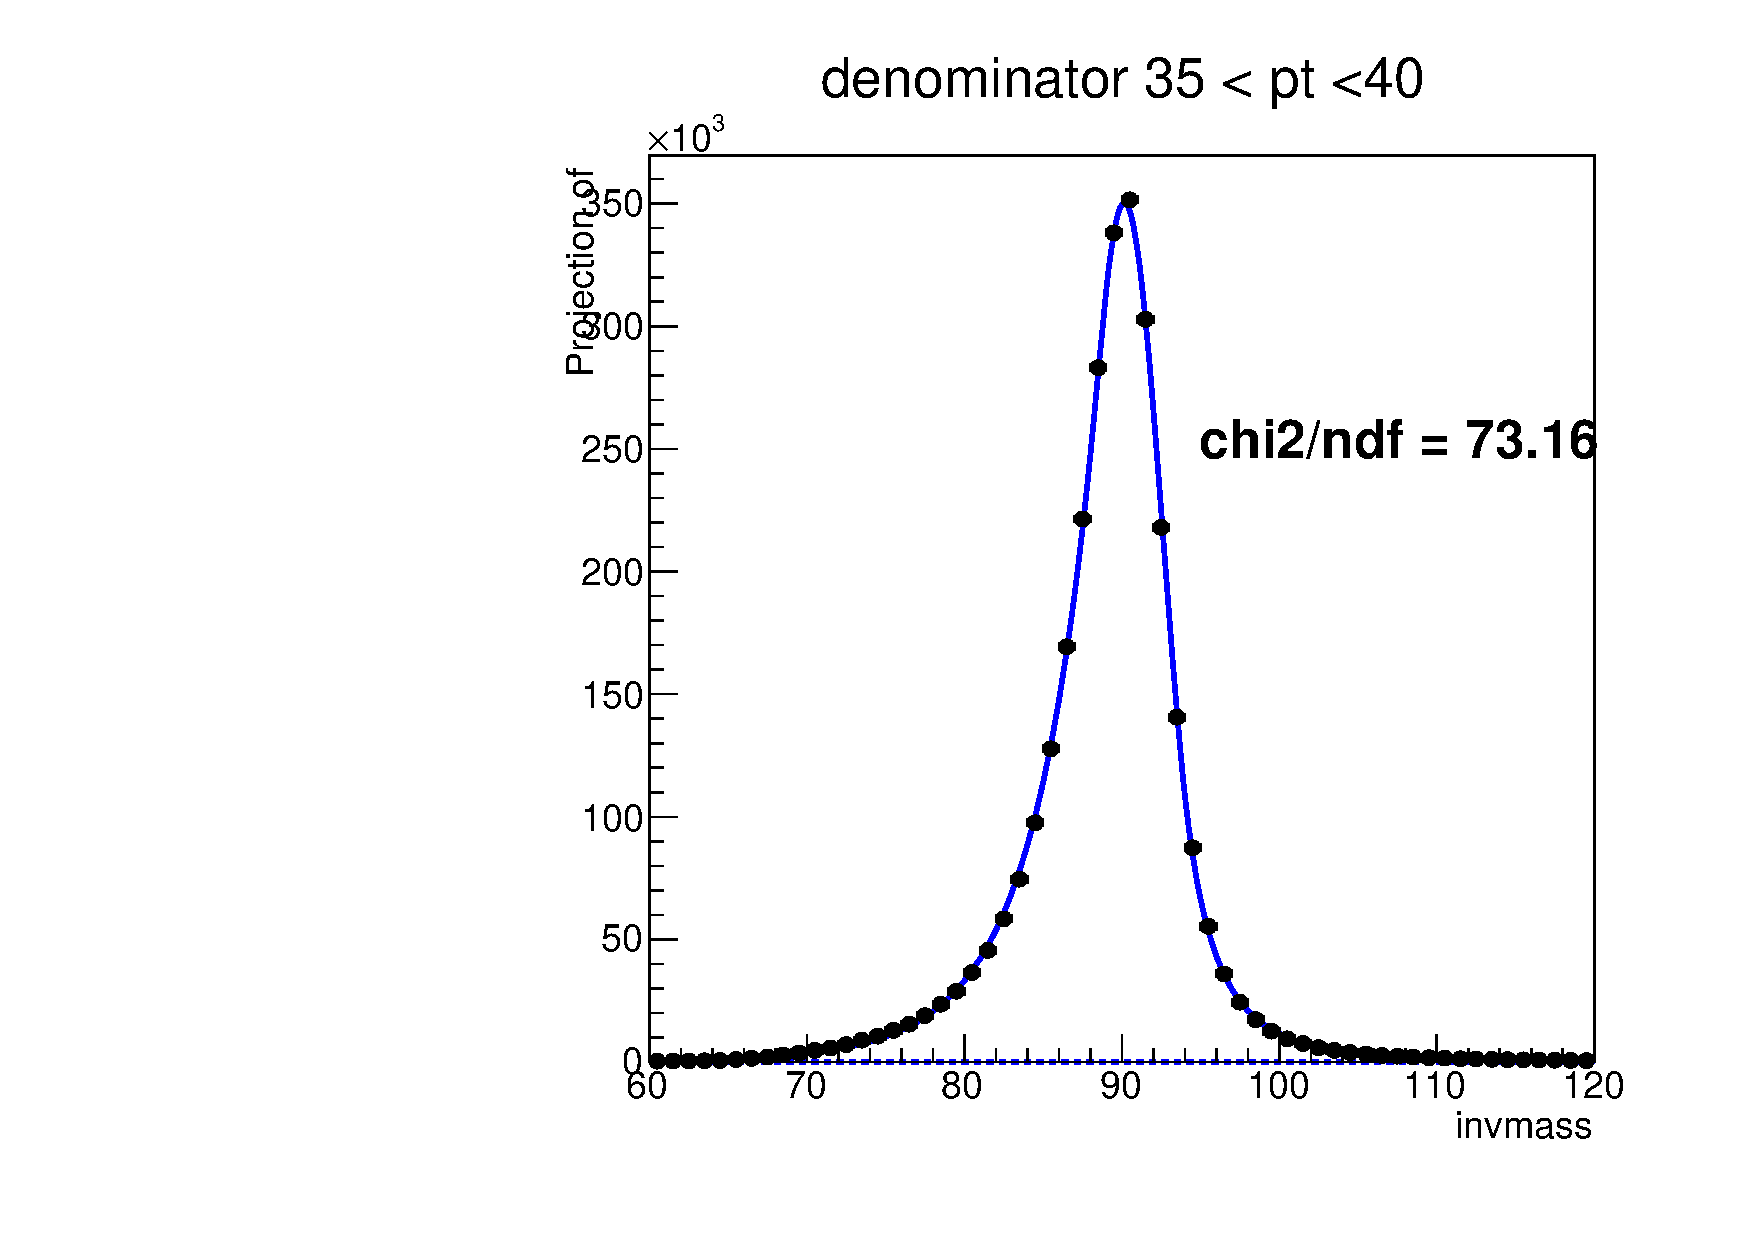
\includegraphics[width=0.24\textwidth]{Figures/Bw_ker_pt_den_35_40.pdf}  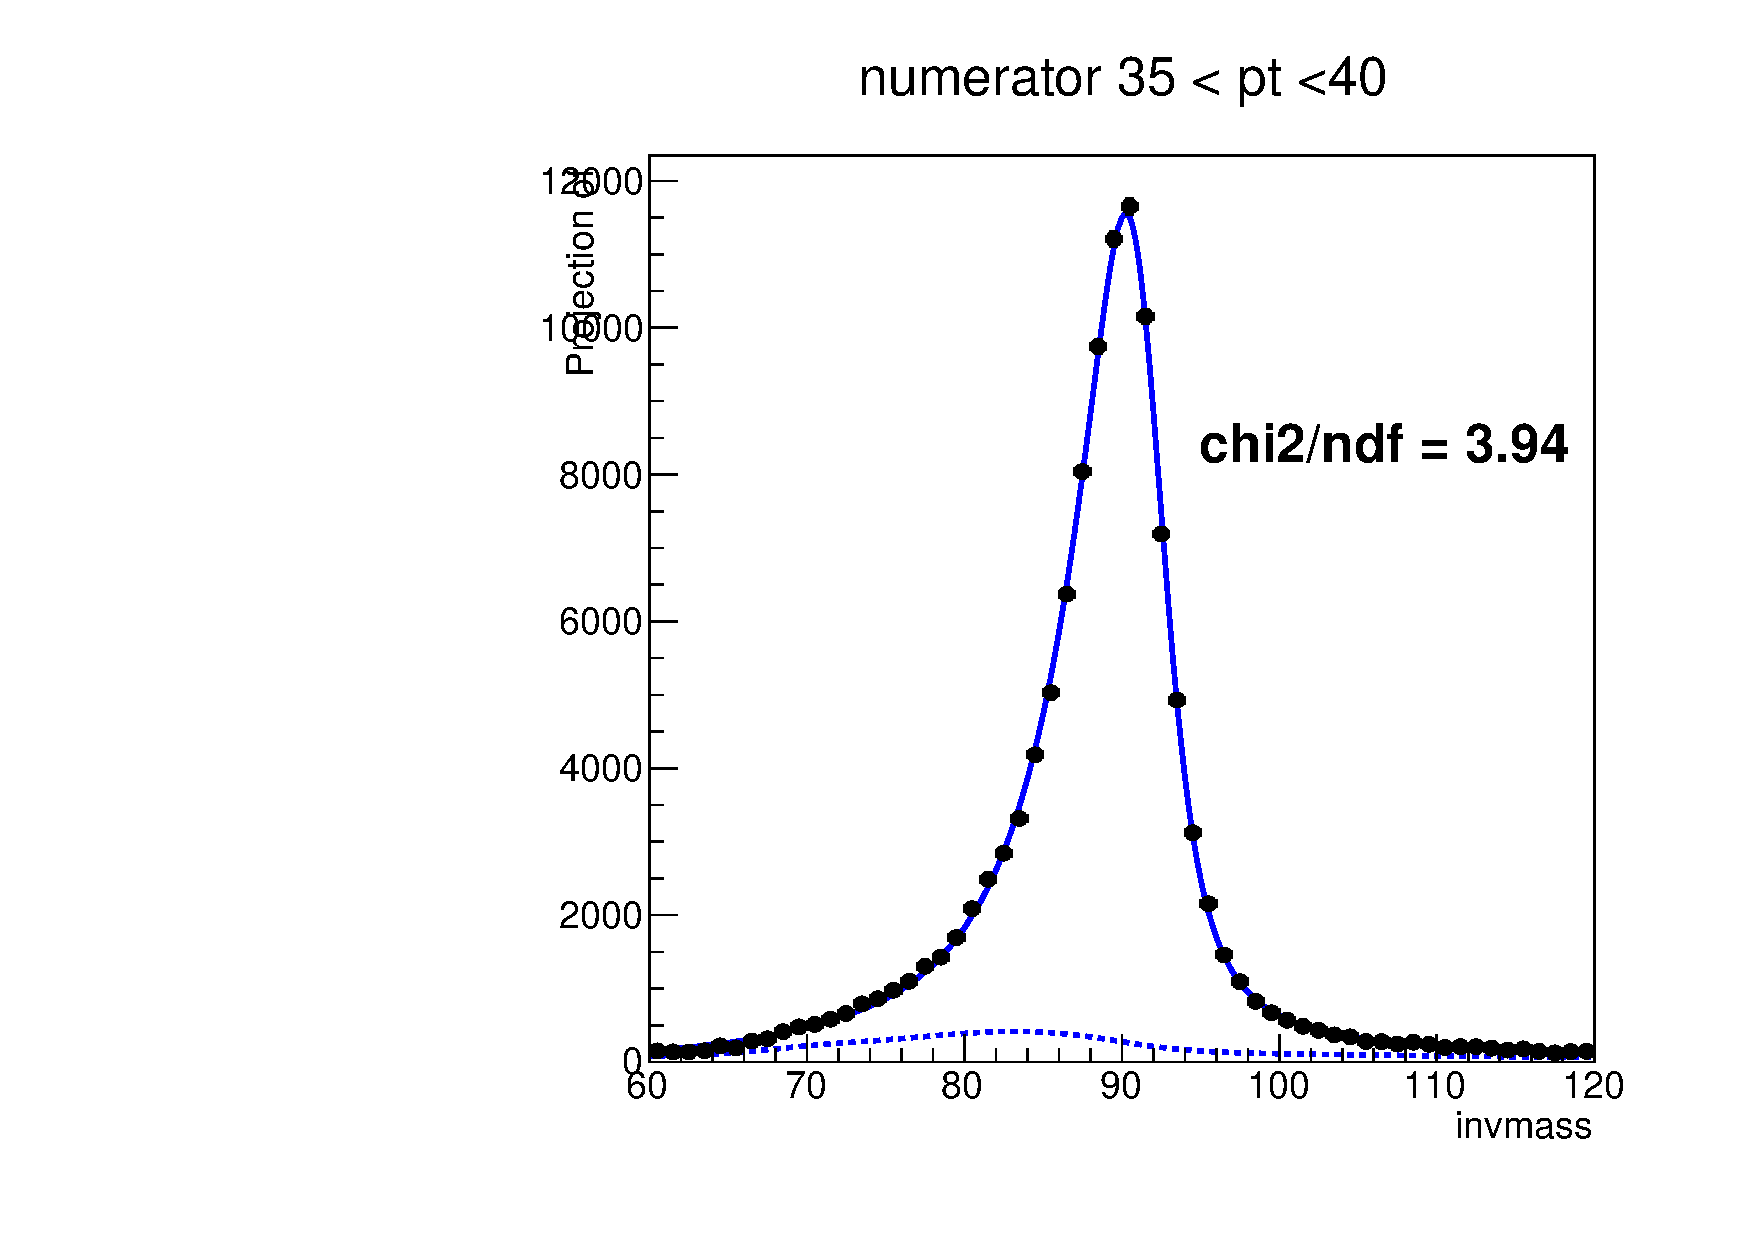
\includegraphics[width=0.24\textwidth]{Figures/Bw_ker_pt_num_35_40.pdf}   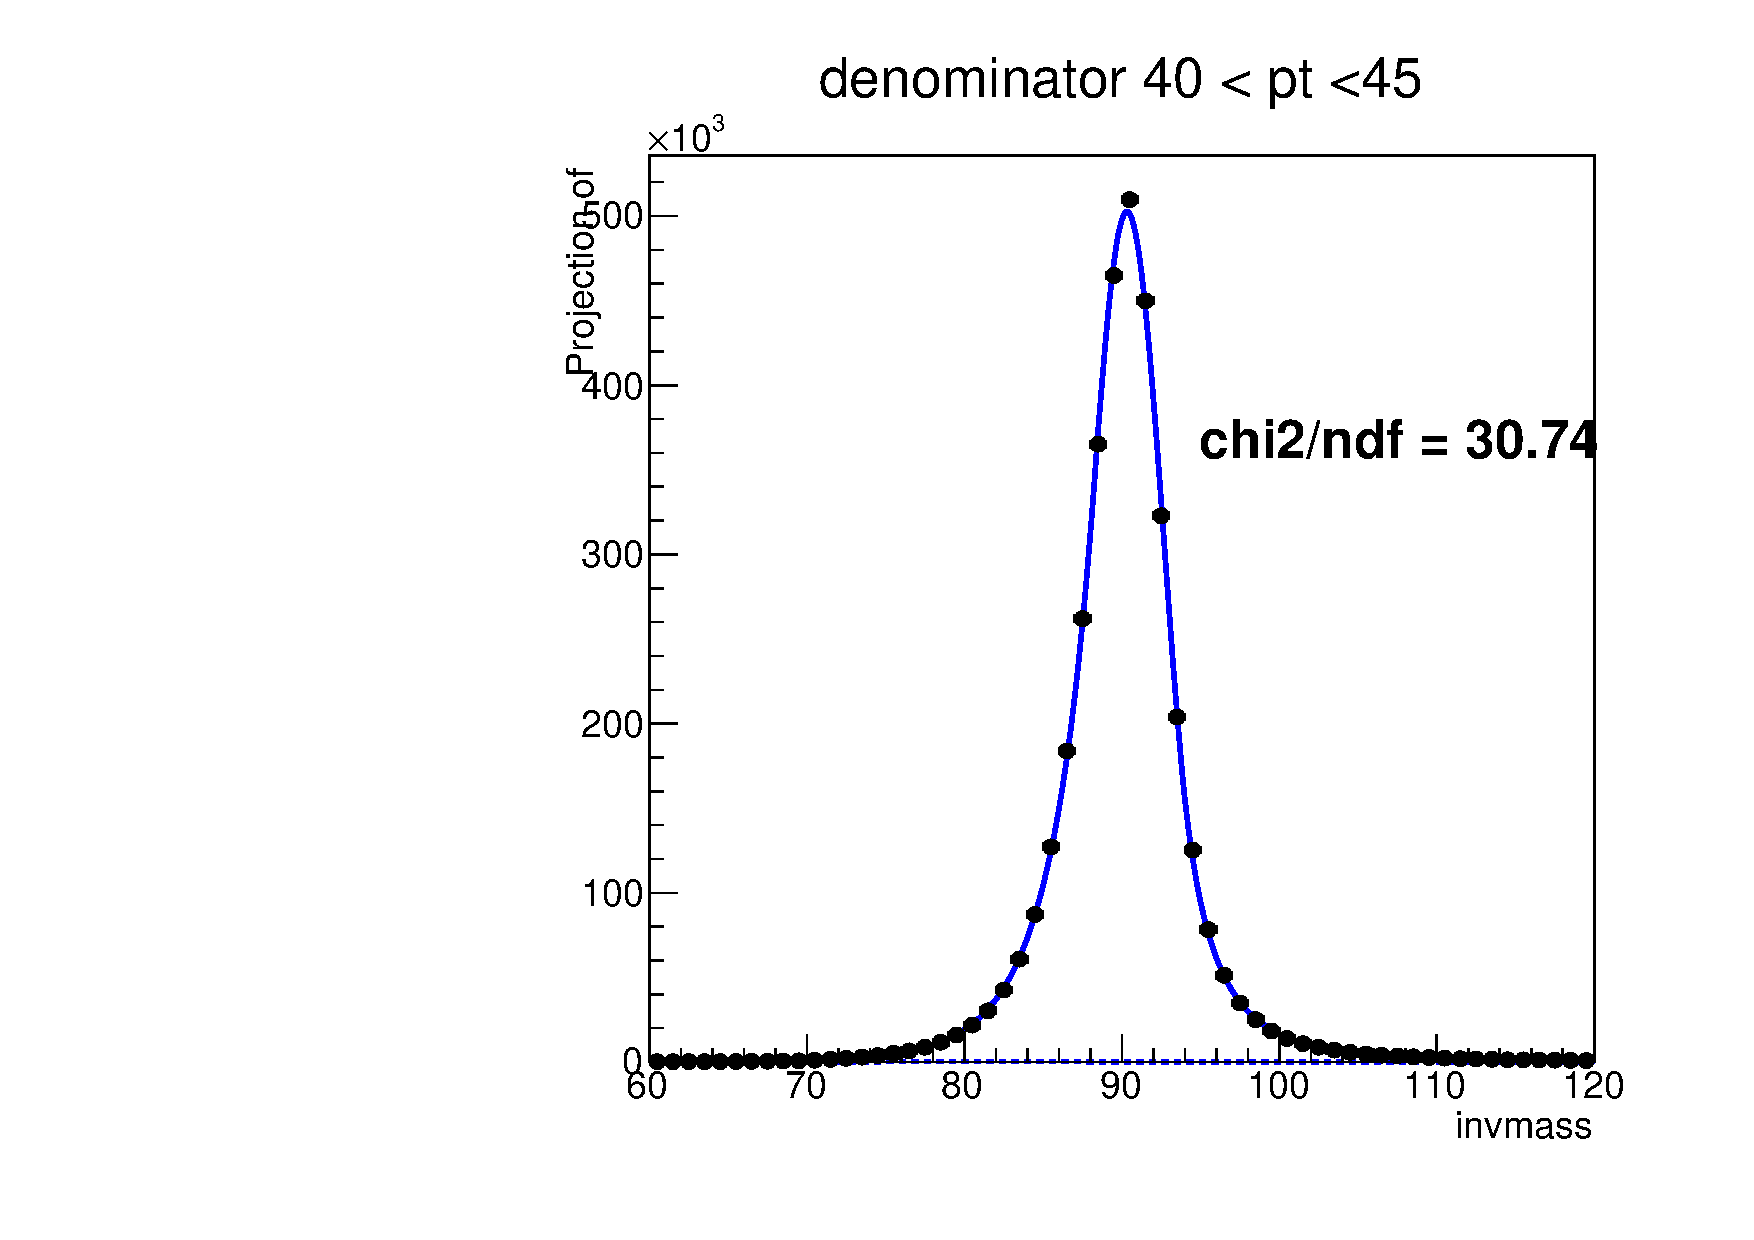
\includegraphics[width=0.24\textwidth]{Figures/Bw_ker_pt_den_40_45.pdf} 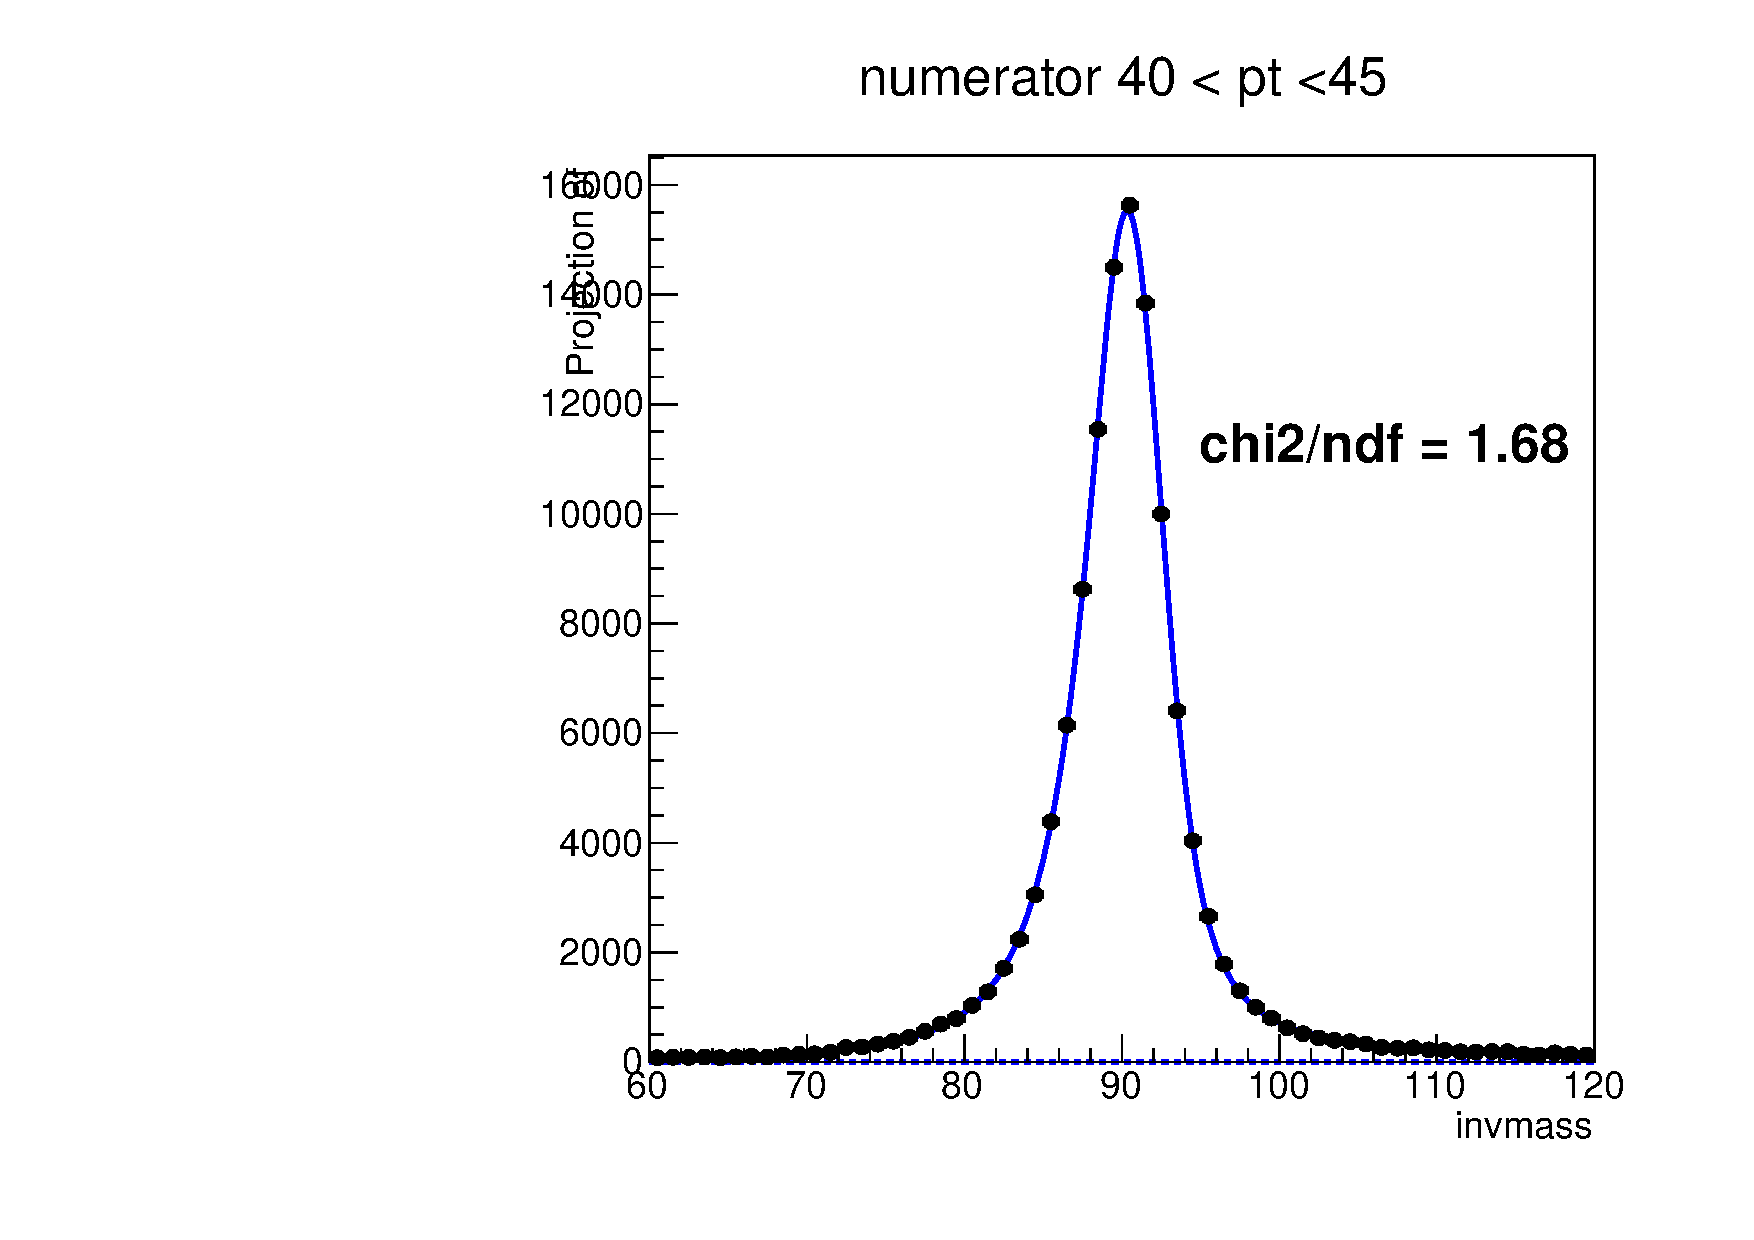
\includegraphics[width=0.24\textwidth]{Figures/Bw_ker_pt_num_40_45.pdf} \\
   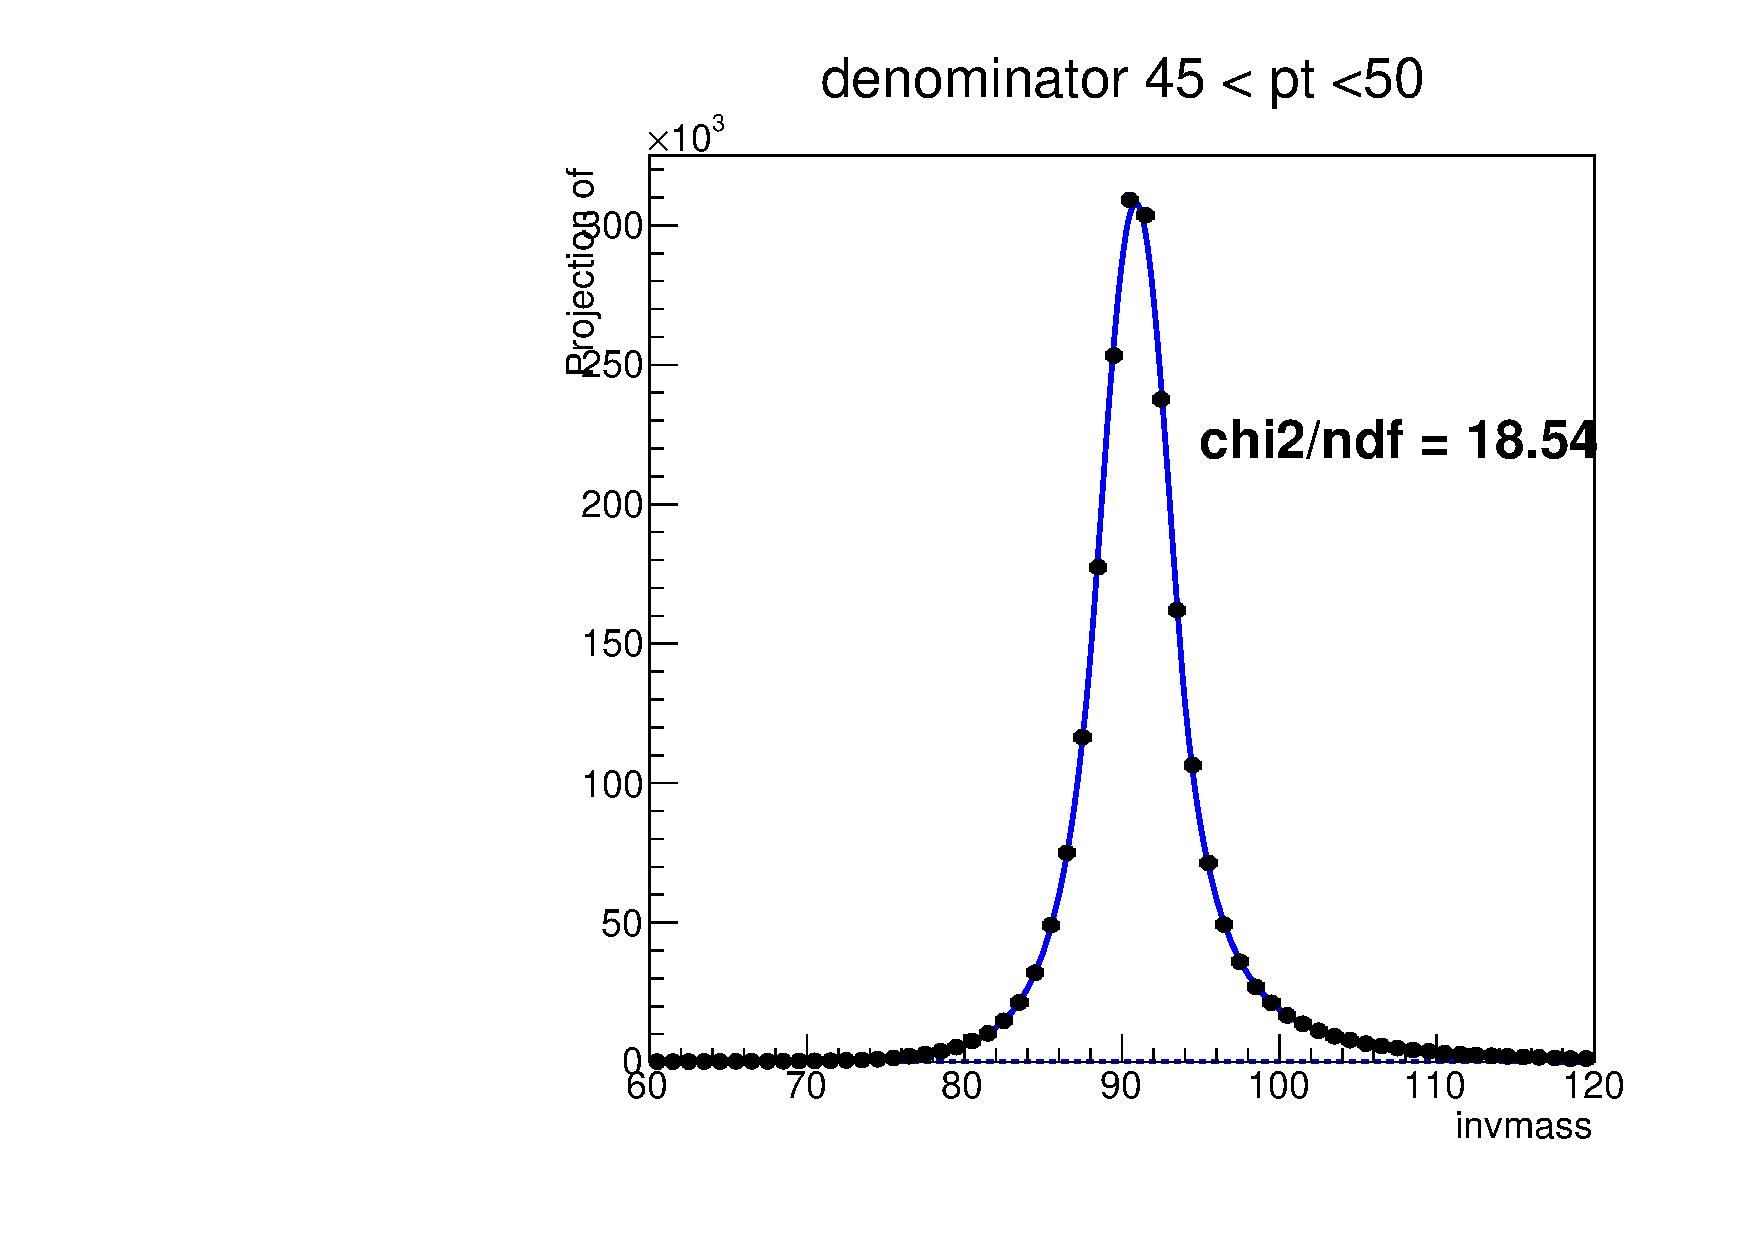
\includegraphics[width=0.24\textwidth]{Figures/Bw_ker_pt_den_45_50.pdf}  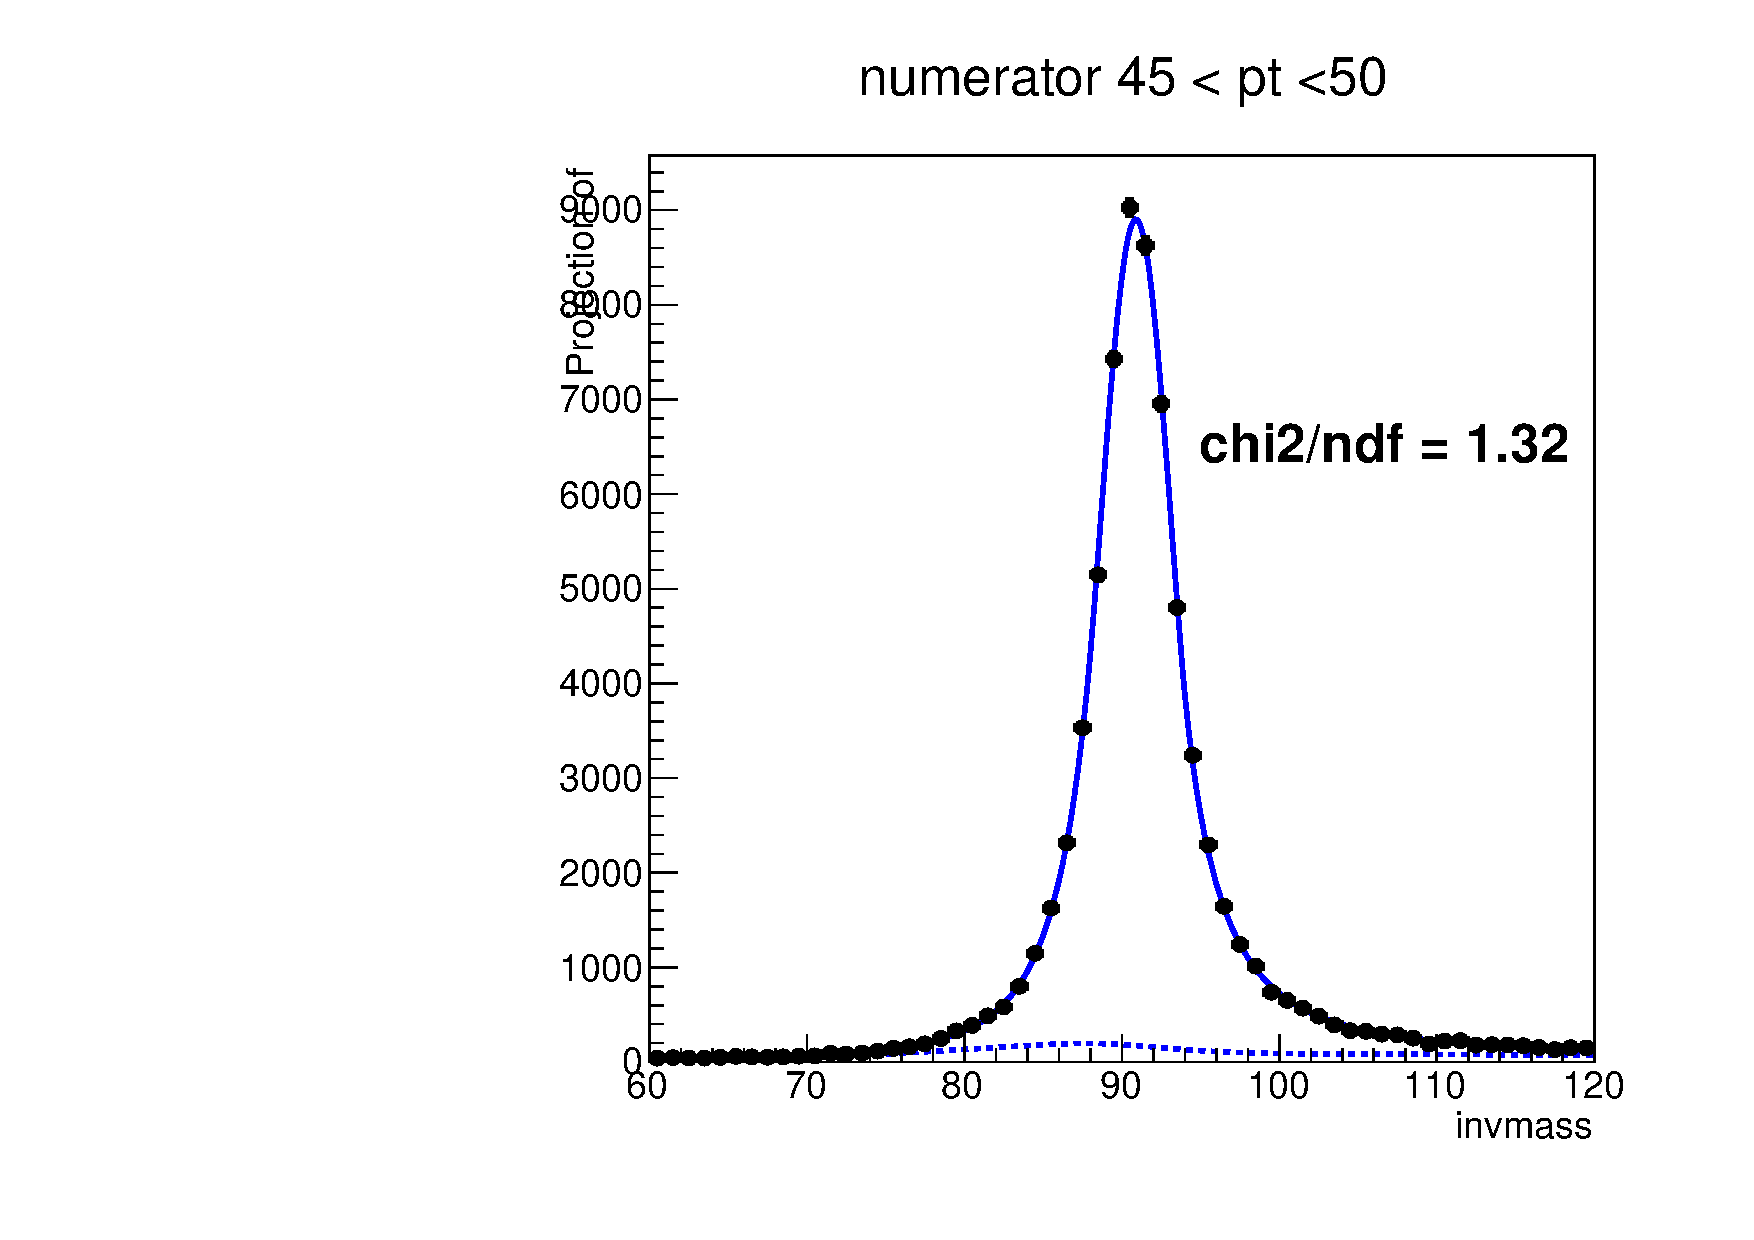
\includegraphics[width=0.24\textwidth]{Figures/Bw_ker_pt_num_45_50.pdf}   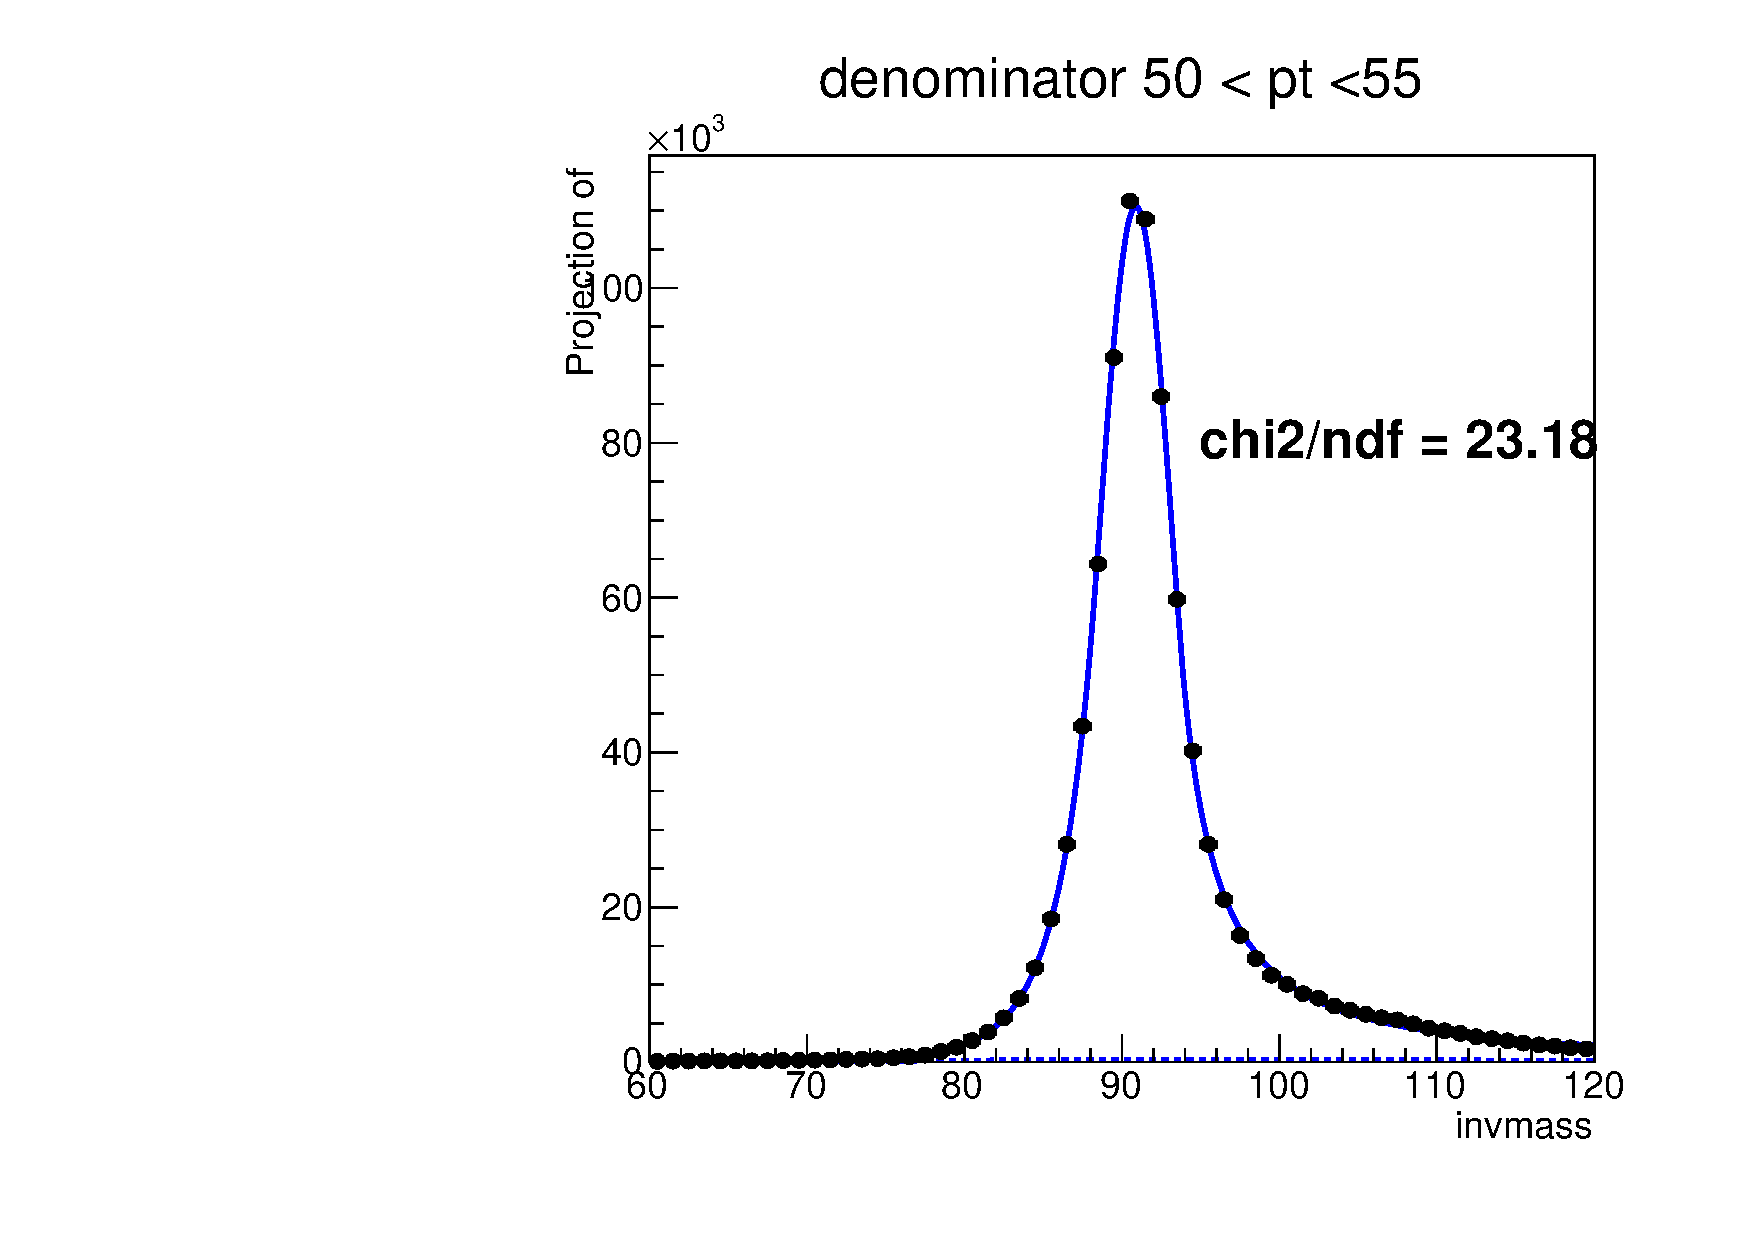
\includegraphics[width=0.24\textwidth]{Figures/Bw_ker_pt_den_50_55.pdf} 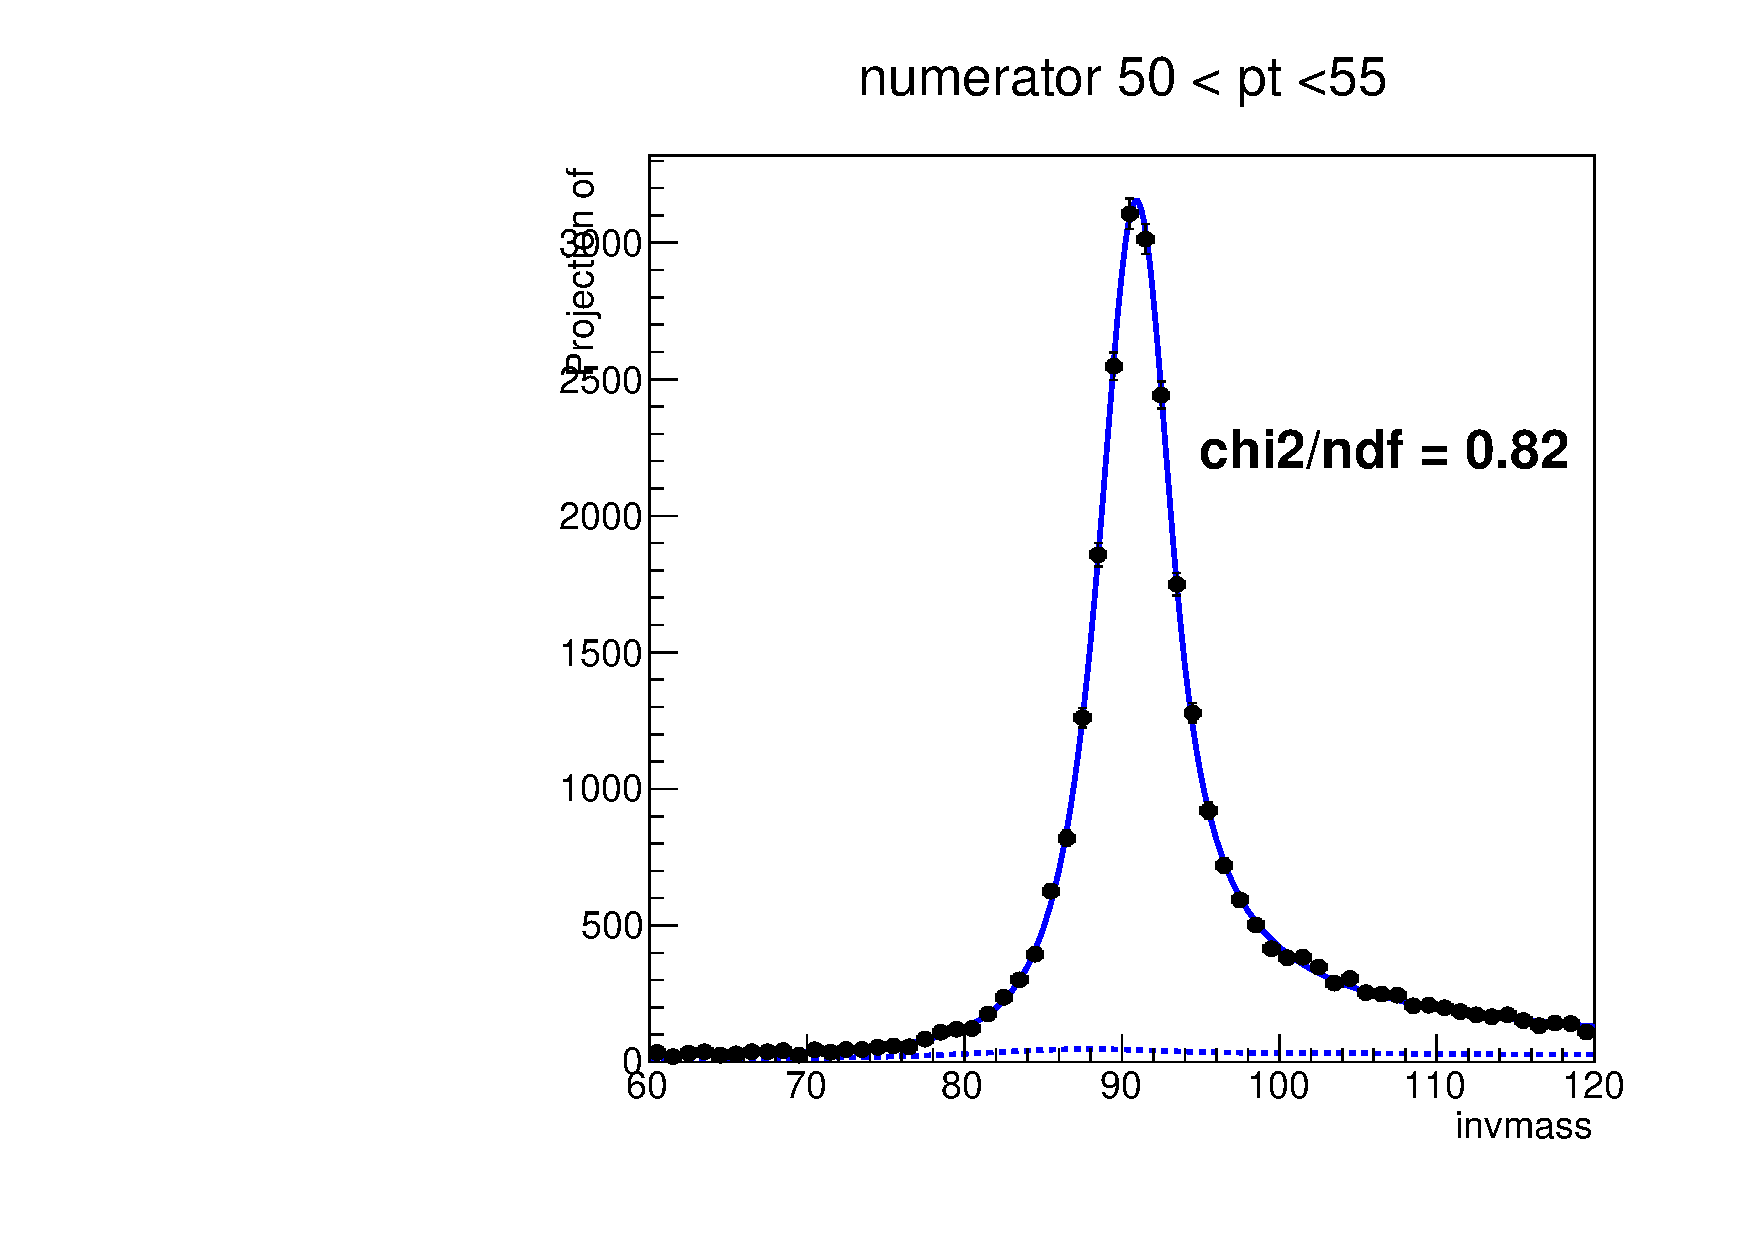
\includegraphics[width=0.24\textwidth]{Figures/Bw_ker_pt_num_50_55.pdf} \\
   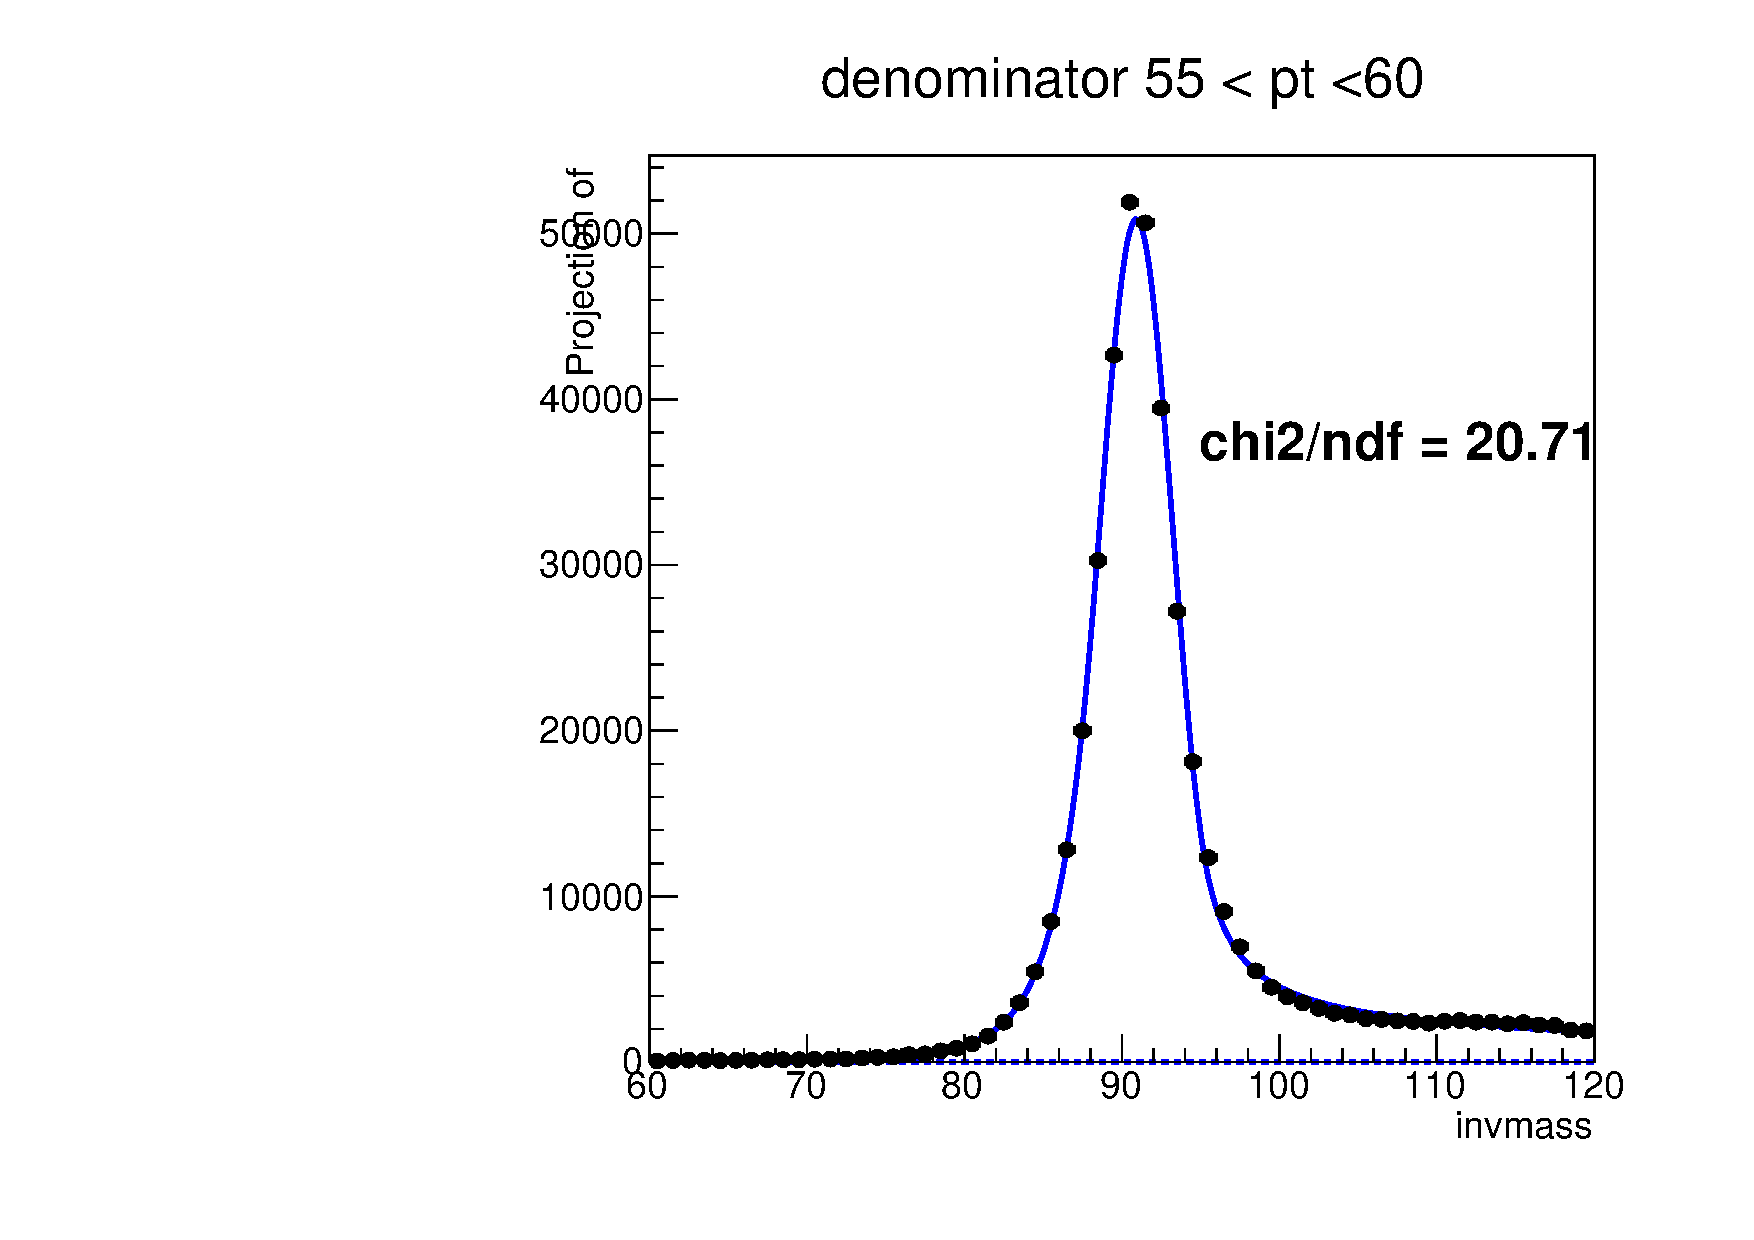
\includegraphics[width=0.24\textwidth]{Figures/Bw_ker_pt_den_55_60.pdf}  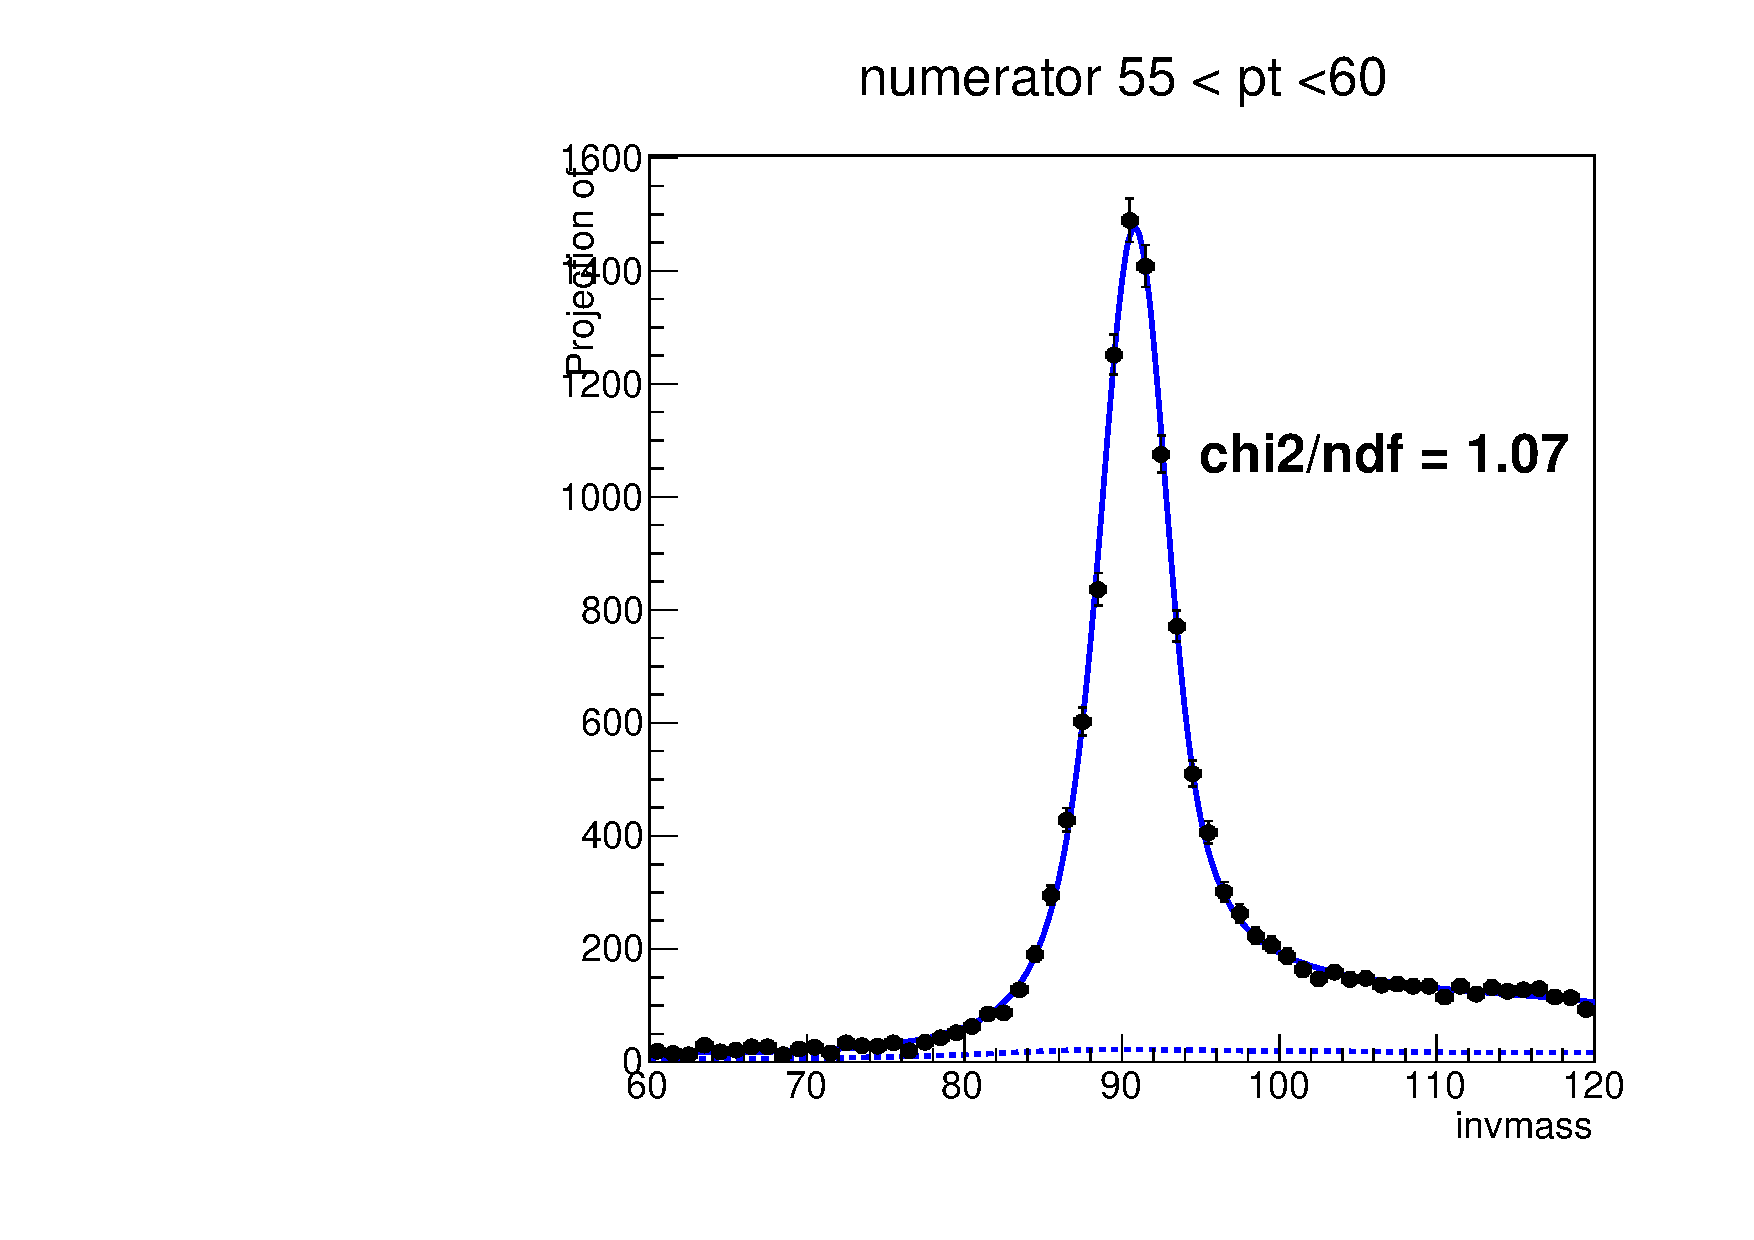
\includegraphics[width=0.24\textwidth]{Figures/Bw_ker_pt_num_55_60.pdf}   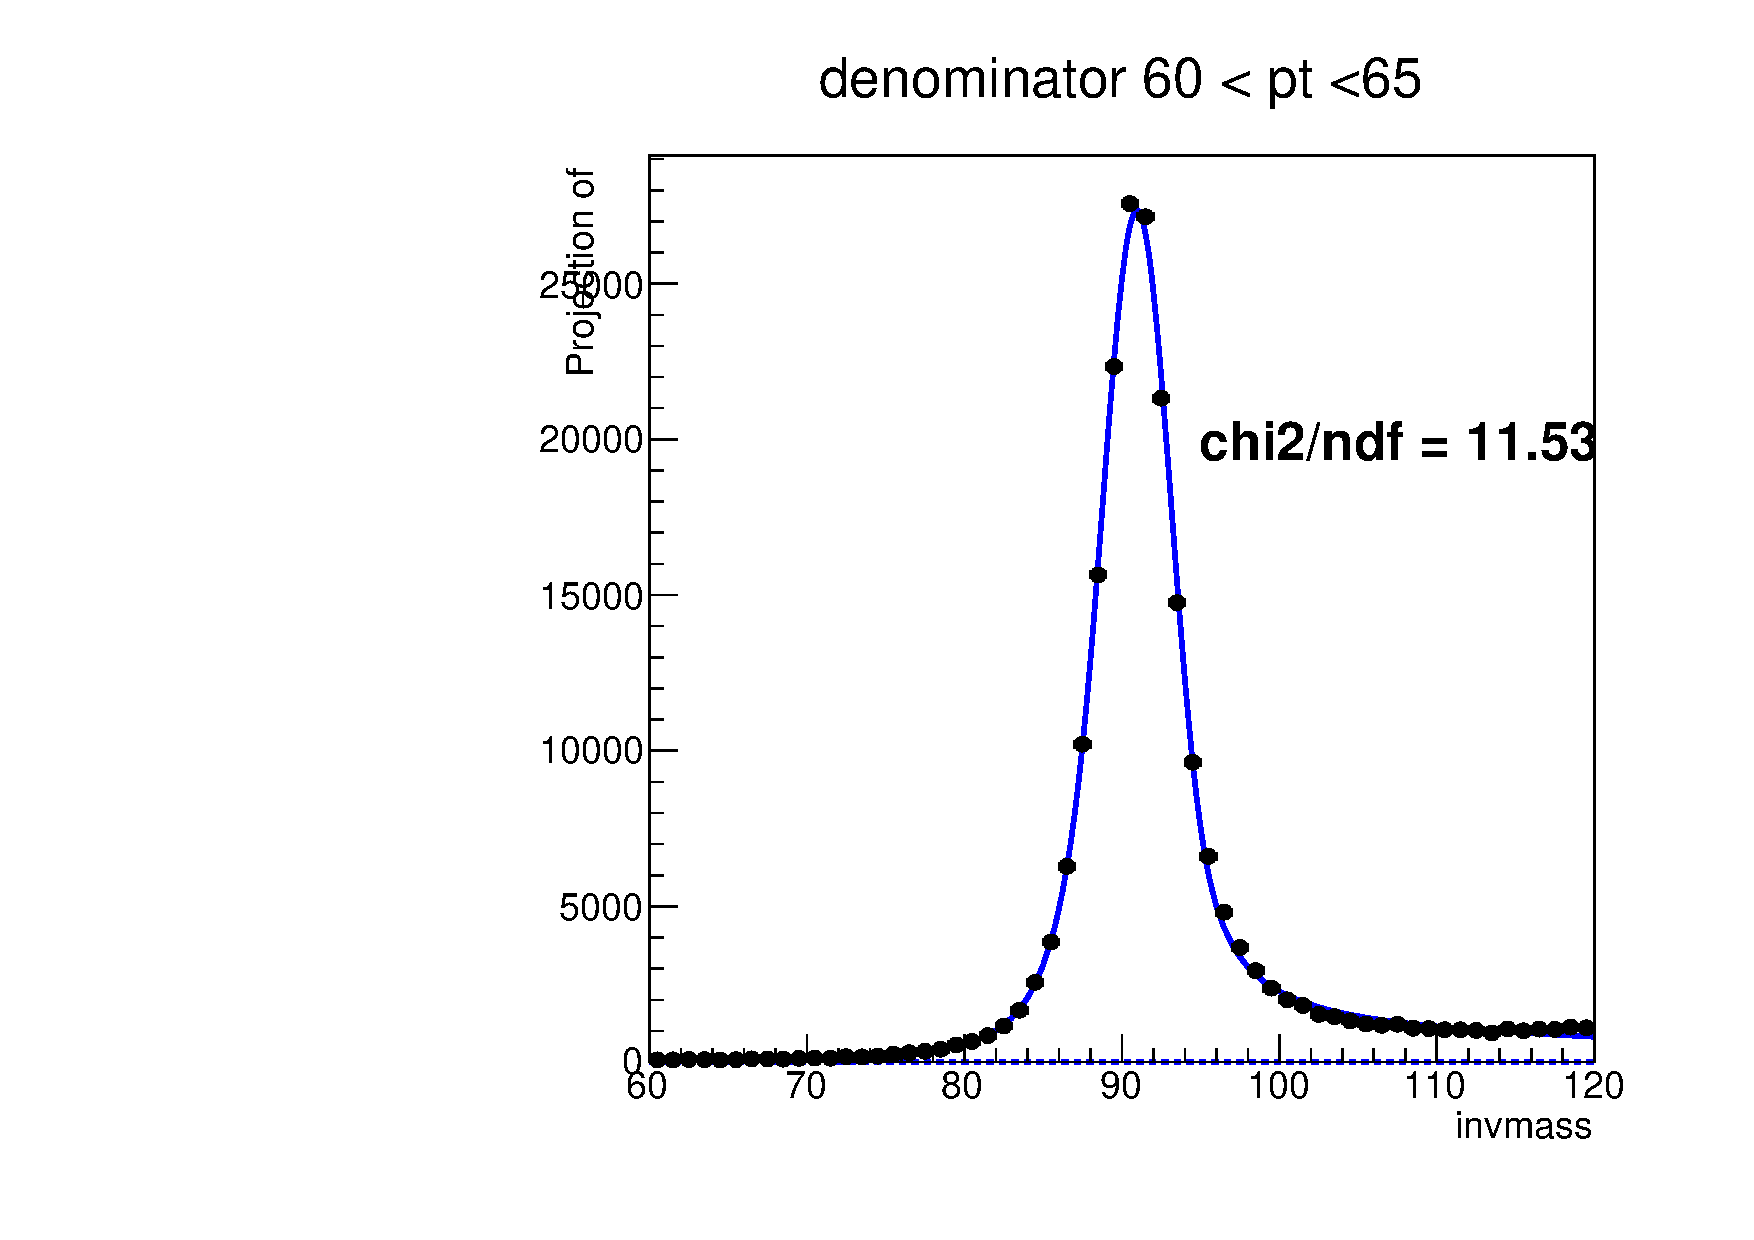
\includegraphics[width=0.24\textwidth]{Figures/Bw_ker_pt_den_60_65.pdf} 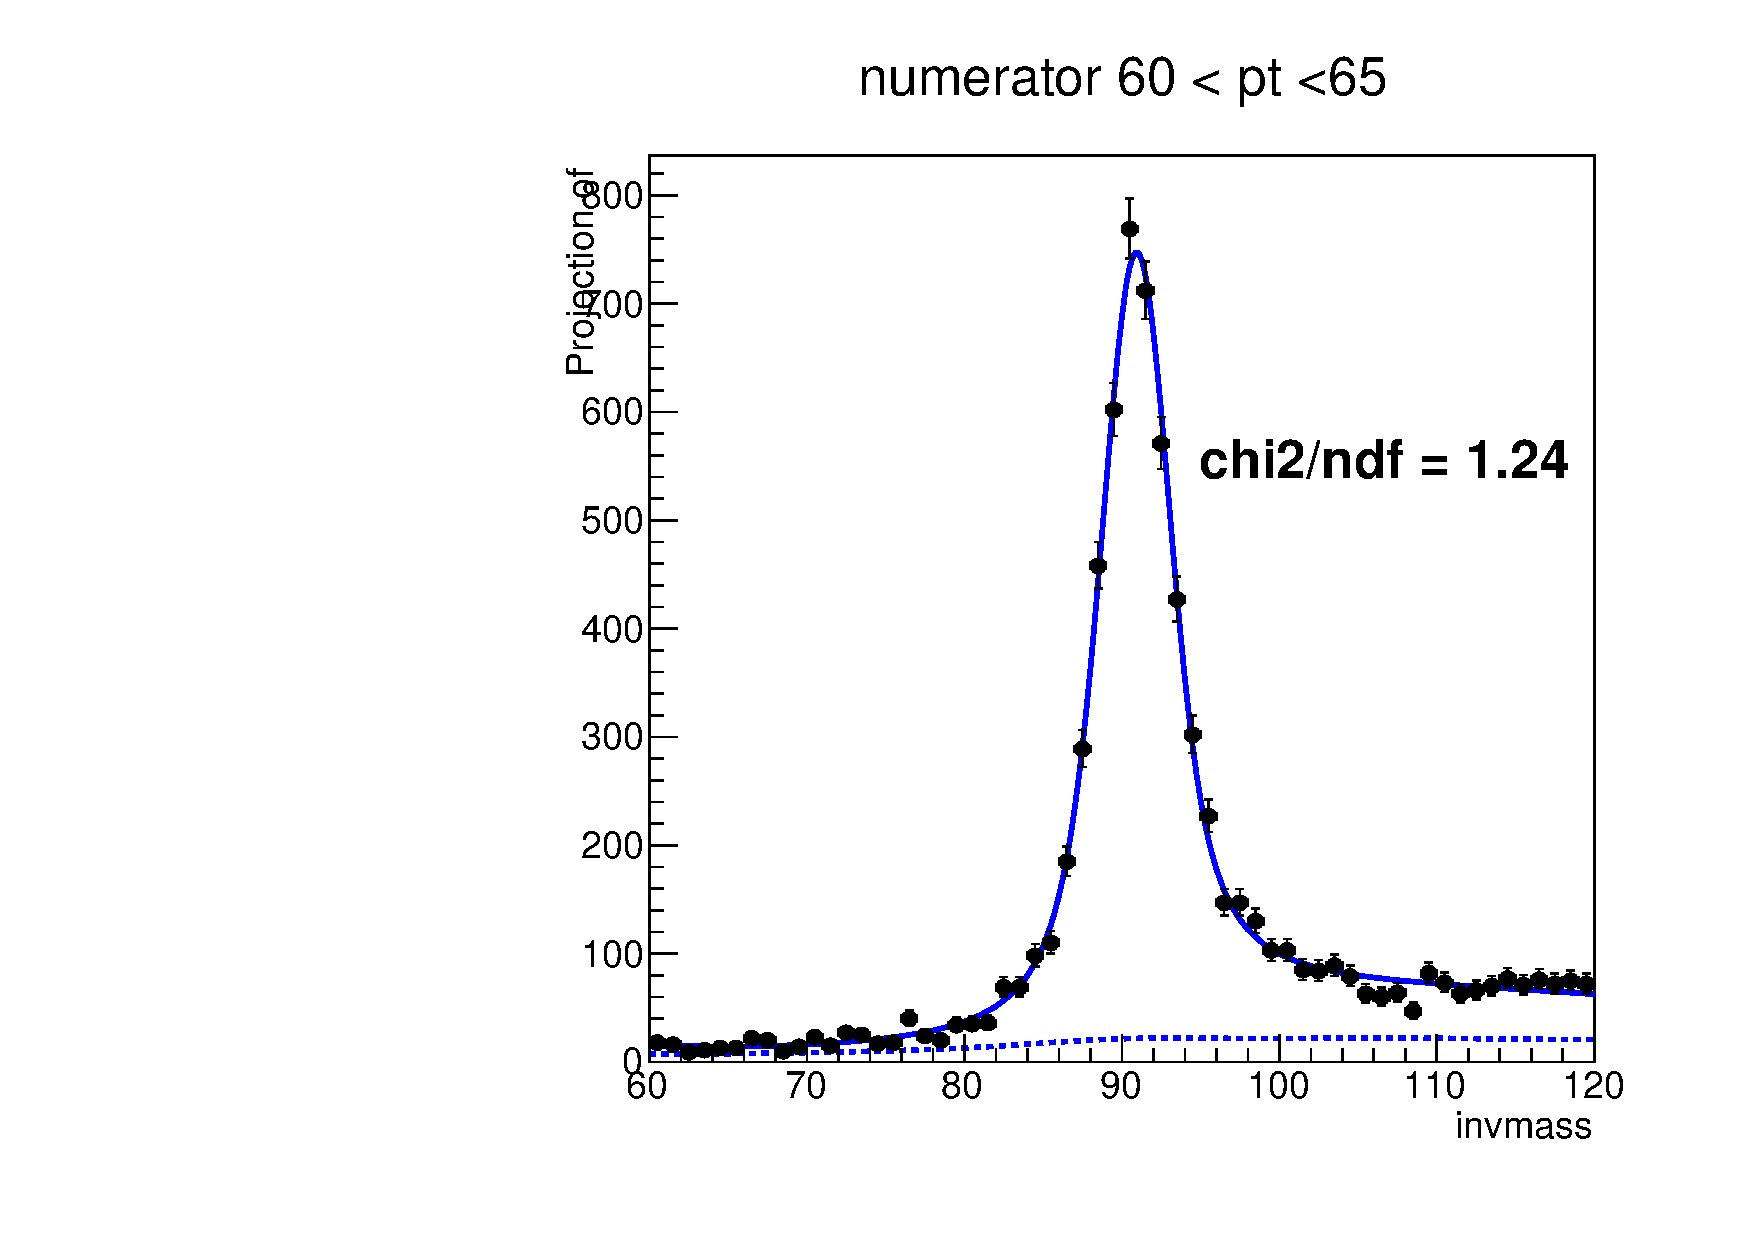
\includegraphics[width=0.24\textwidth]{Figures/Bw_ker_pt_num_60_65.pdf} \\
   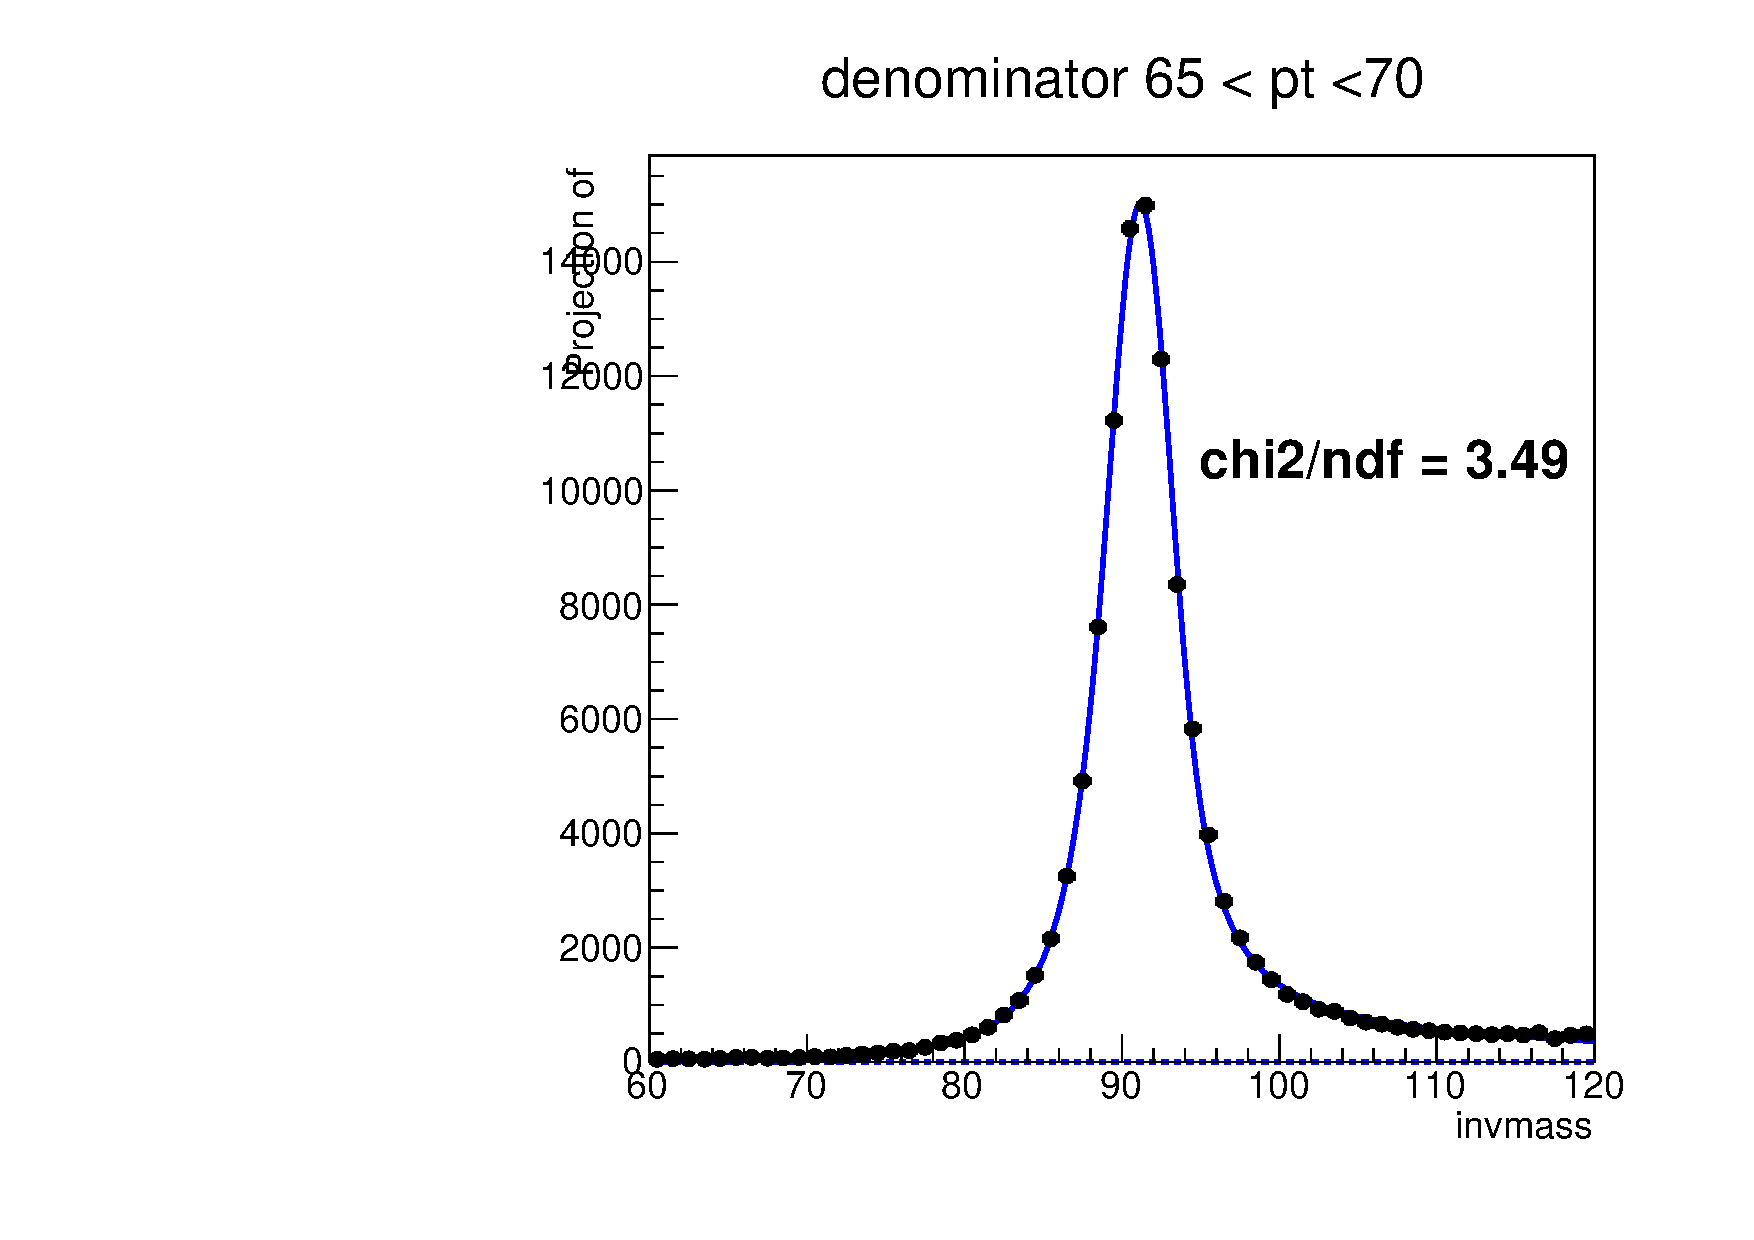
\includegraphics[width=0.24\textwidth]{Figures/Bw_ker_pt_den_65_70.pdf}  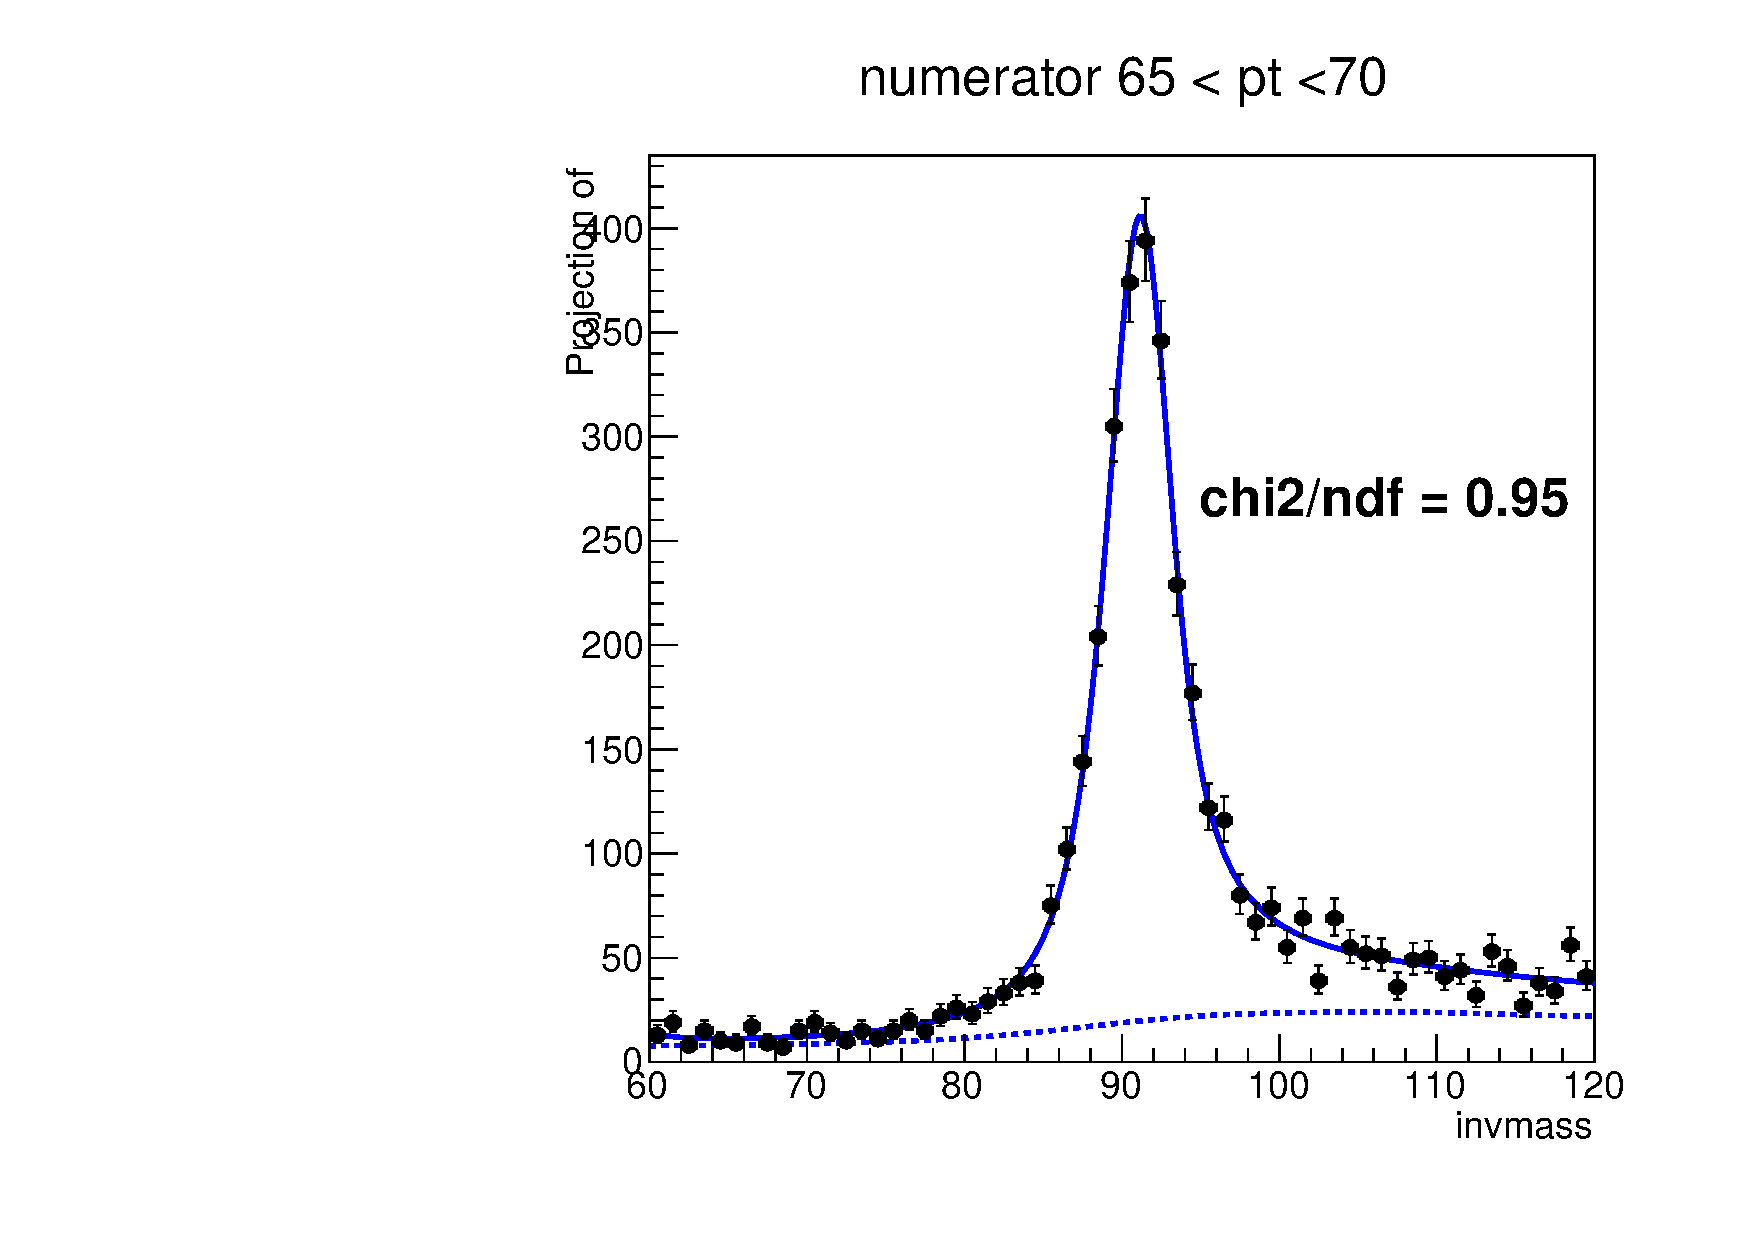
\includegraphics[width=0.24\textwidth]{Figures/Bw_ker_pt_num_65_70.pdf}   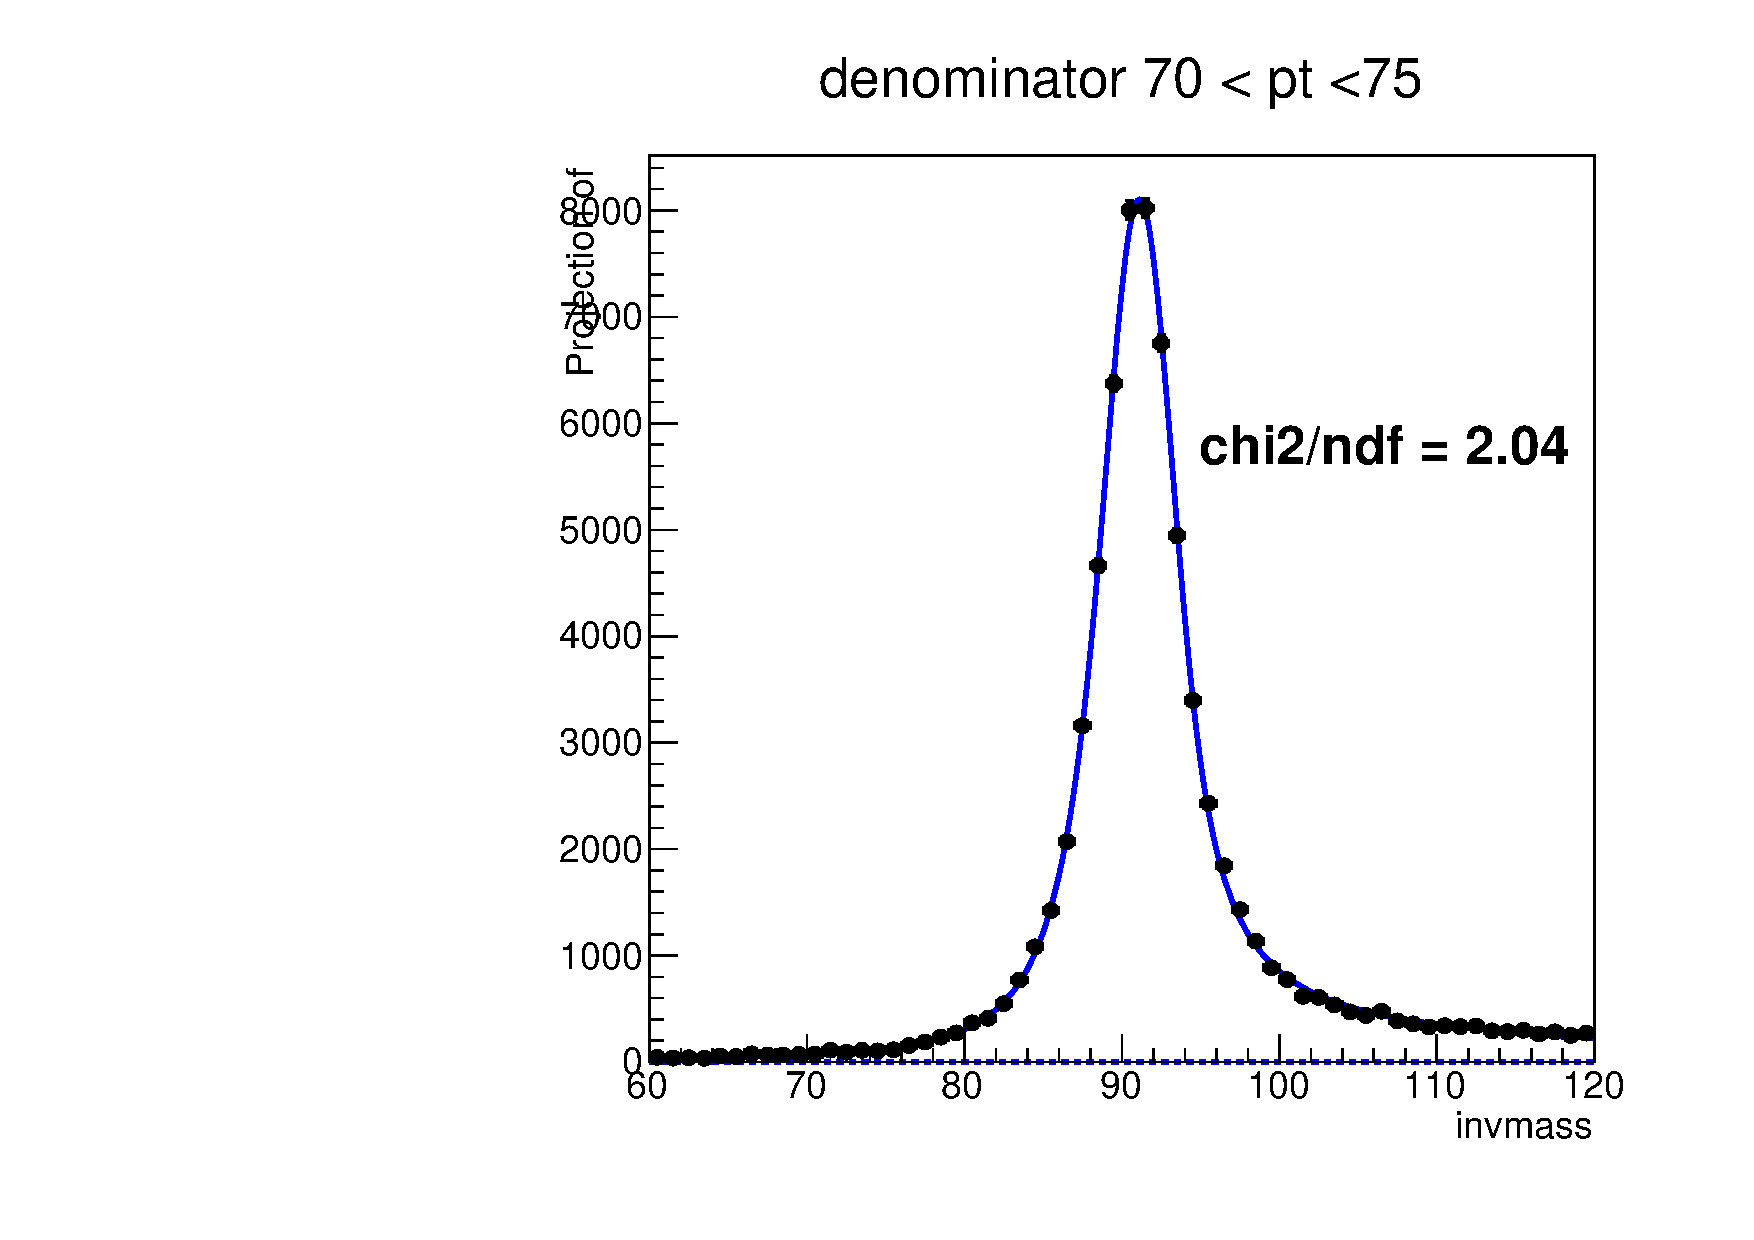
\includegraphics[width=0.24\textwidth]{Figures/Bw_ker_pt_den_70_75.pdf} 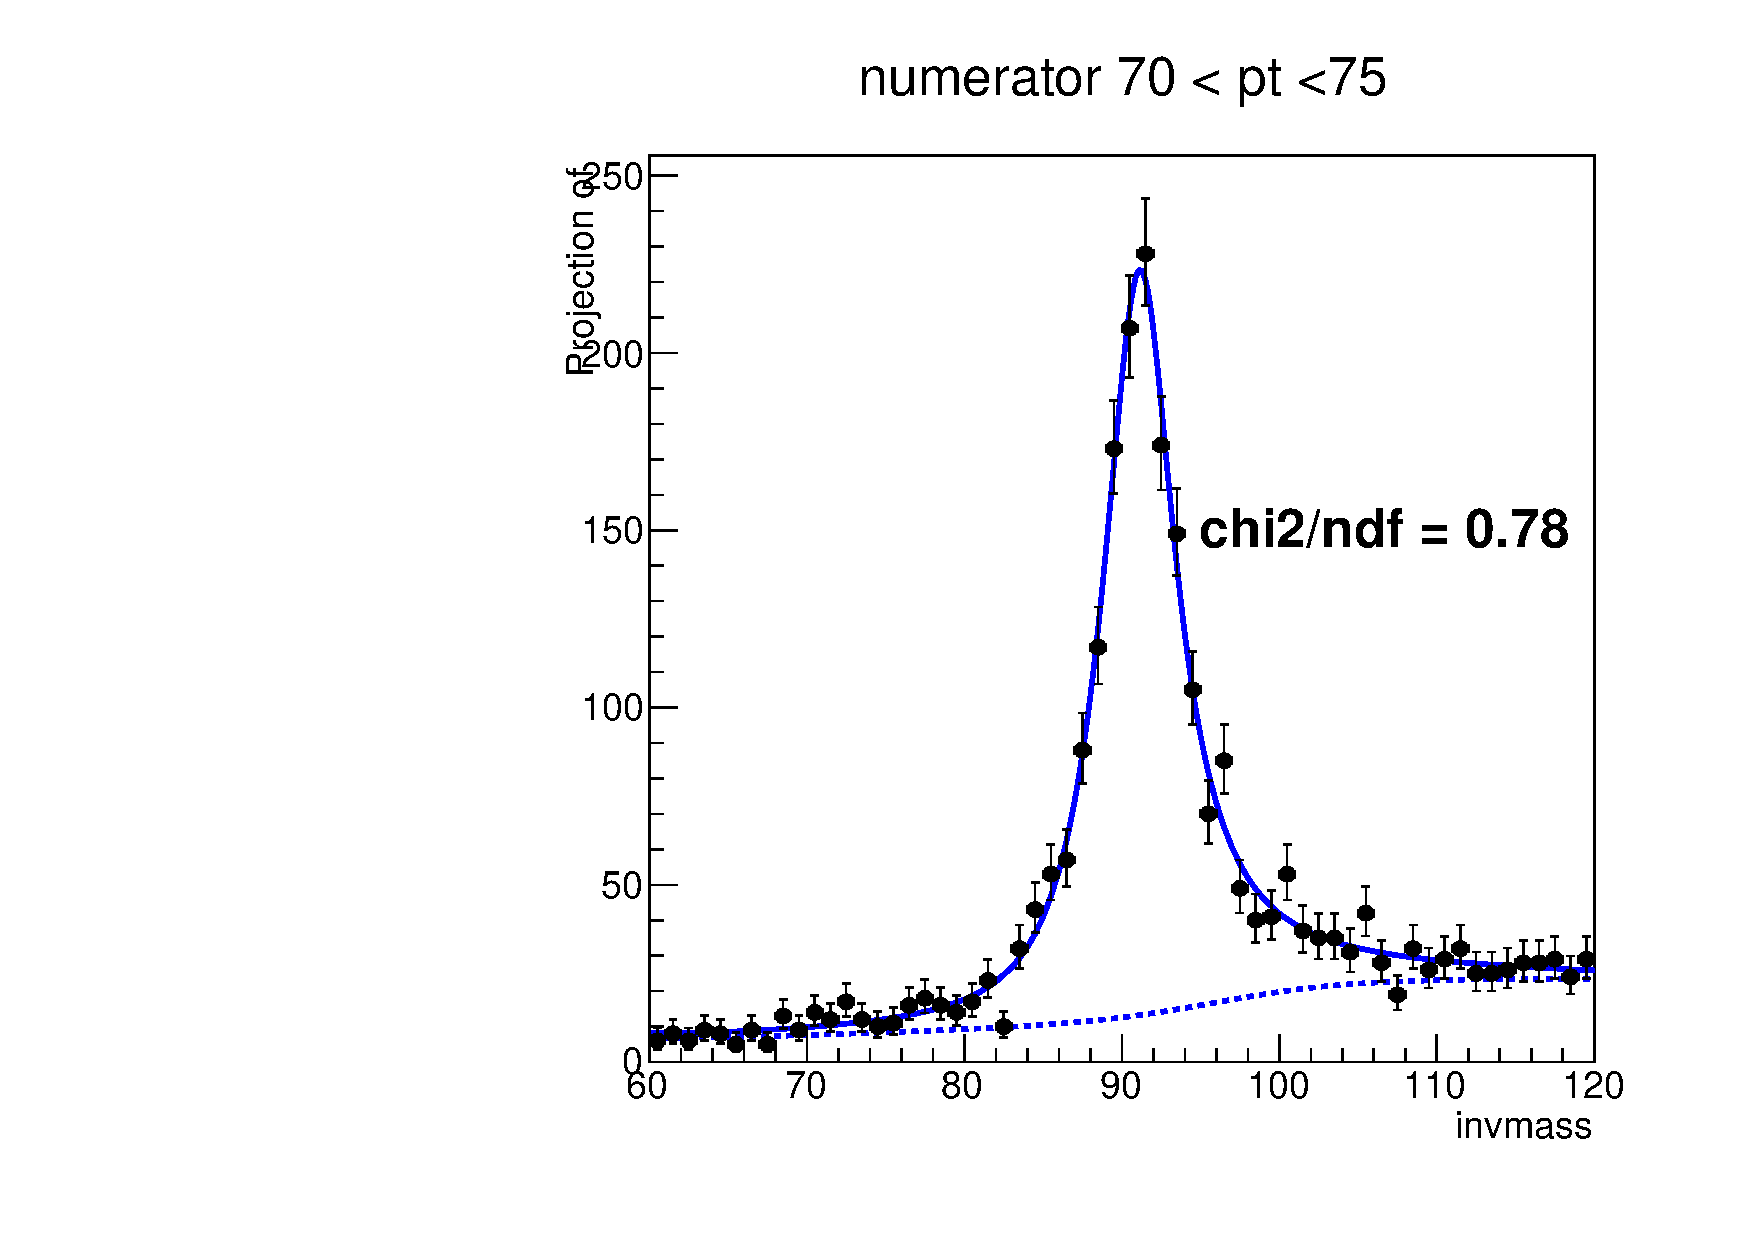
\includegraphics[width=0.24\textwidth]{Figures/Bw_ker_pt_num_70_75.pdf} \\
   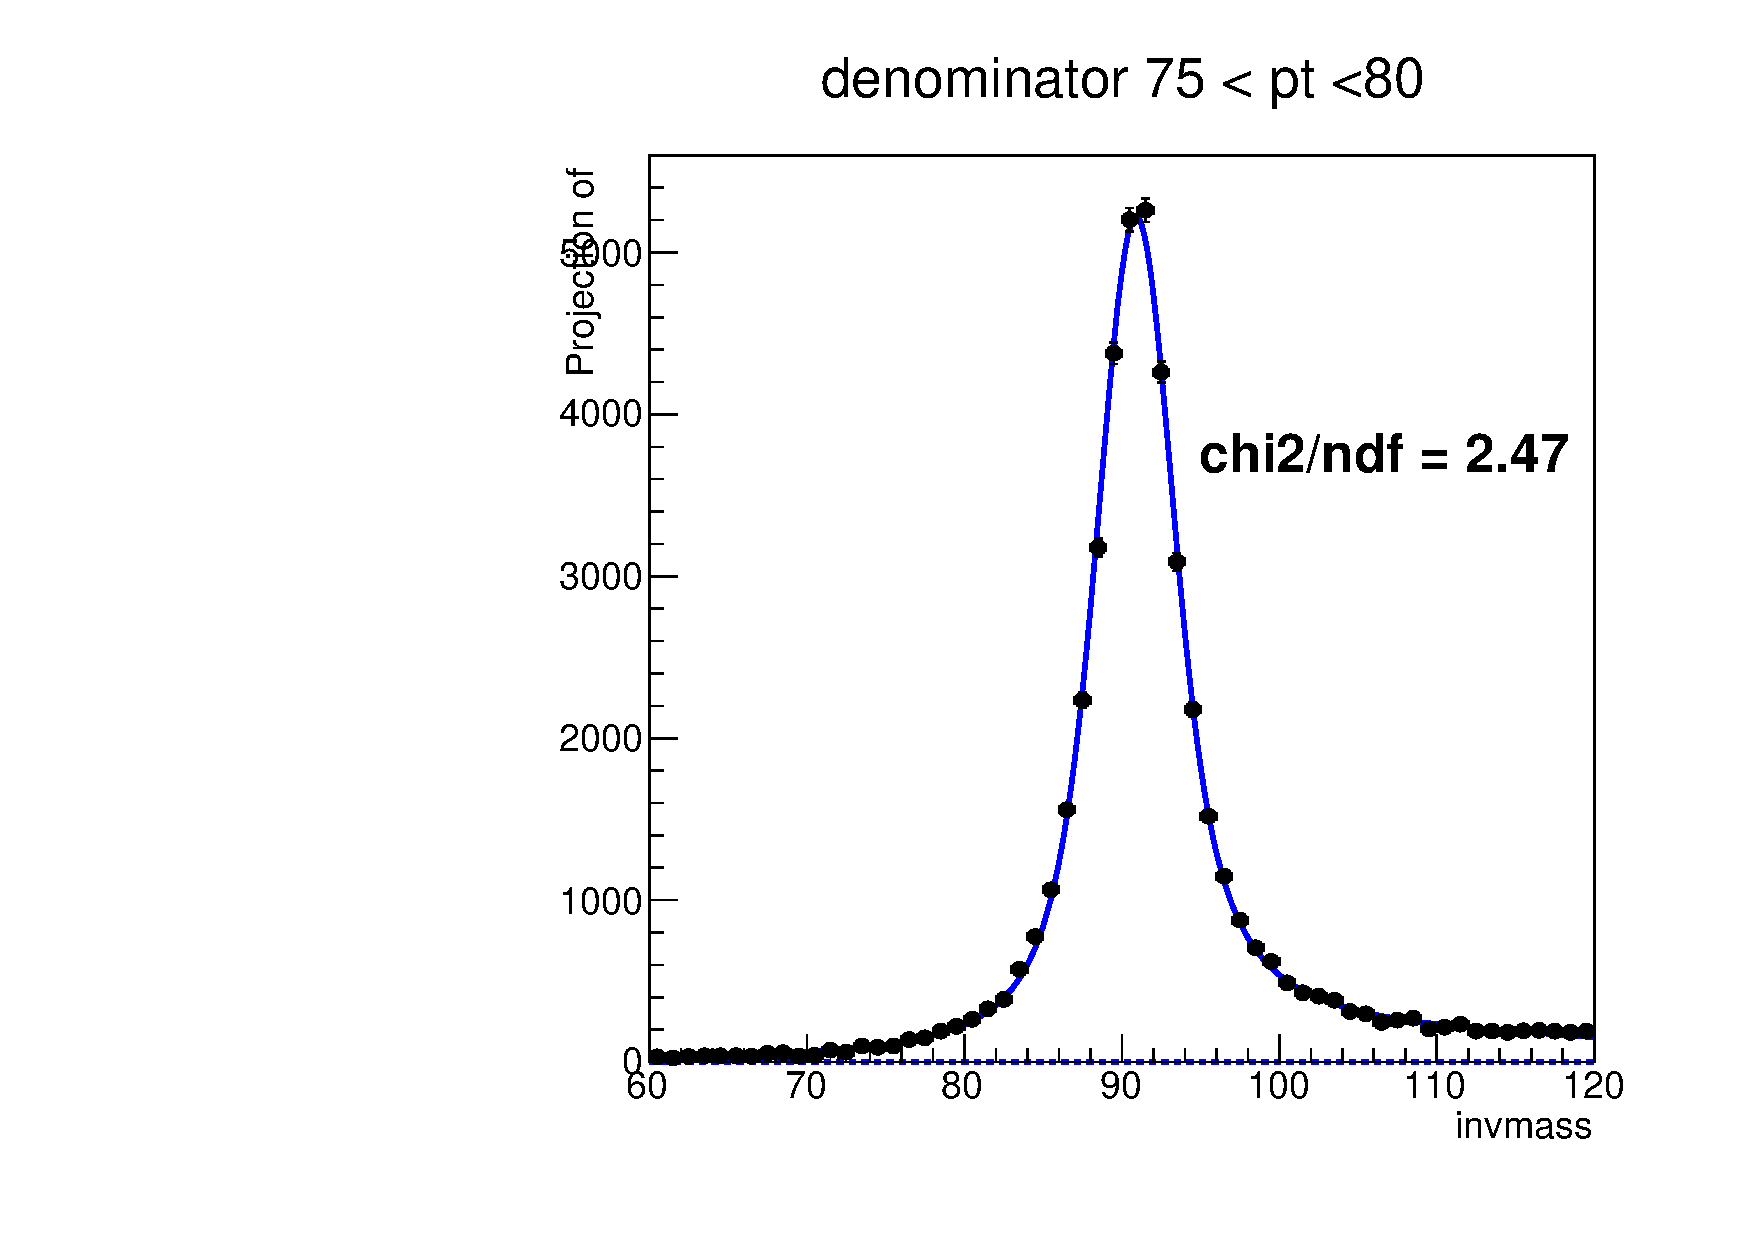
\includegraphics[width=0.24\textwidth]{Figures/Bw_ker_pt_den_75_80.pdf}  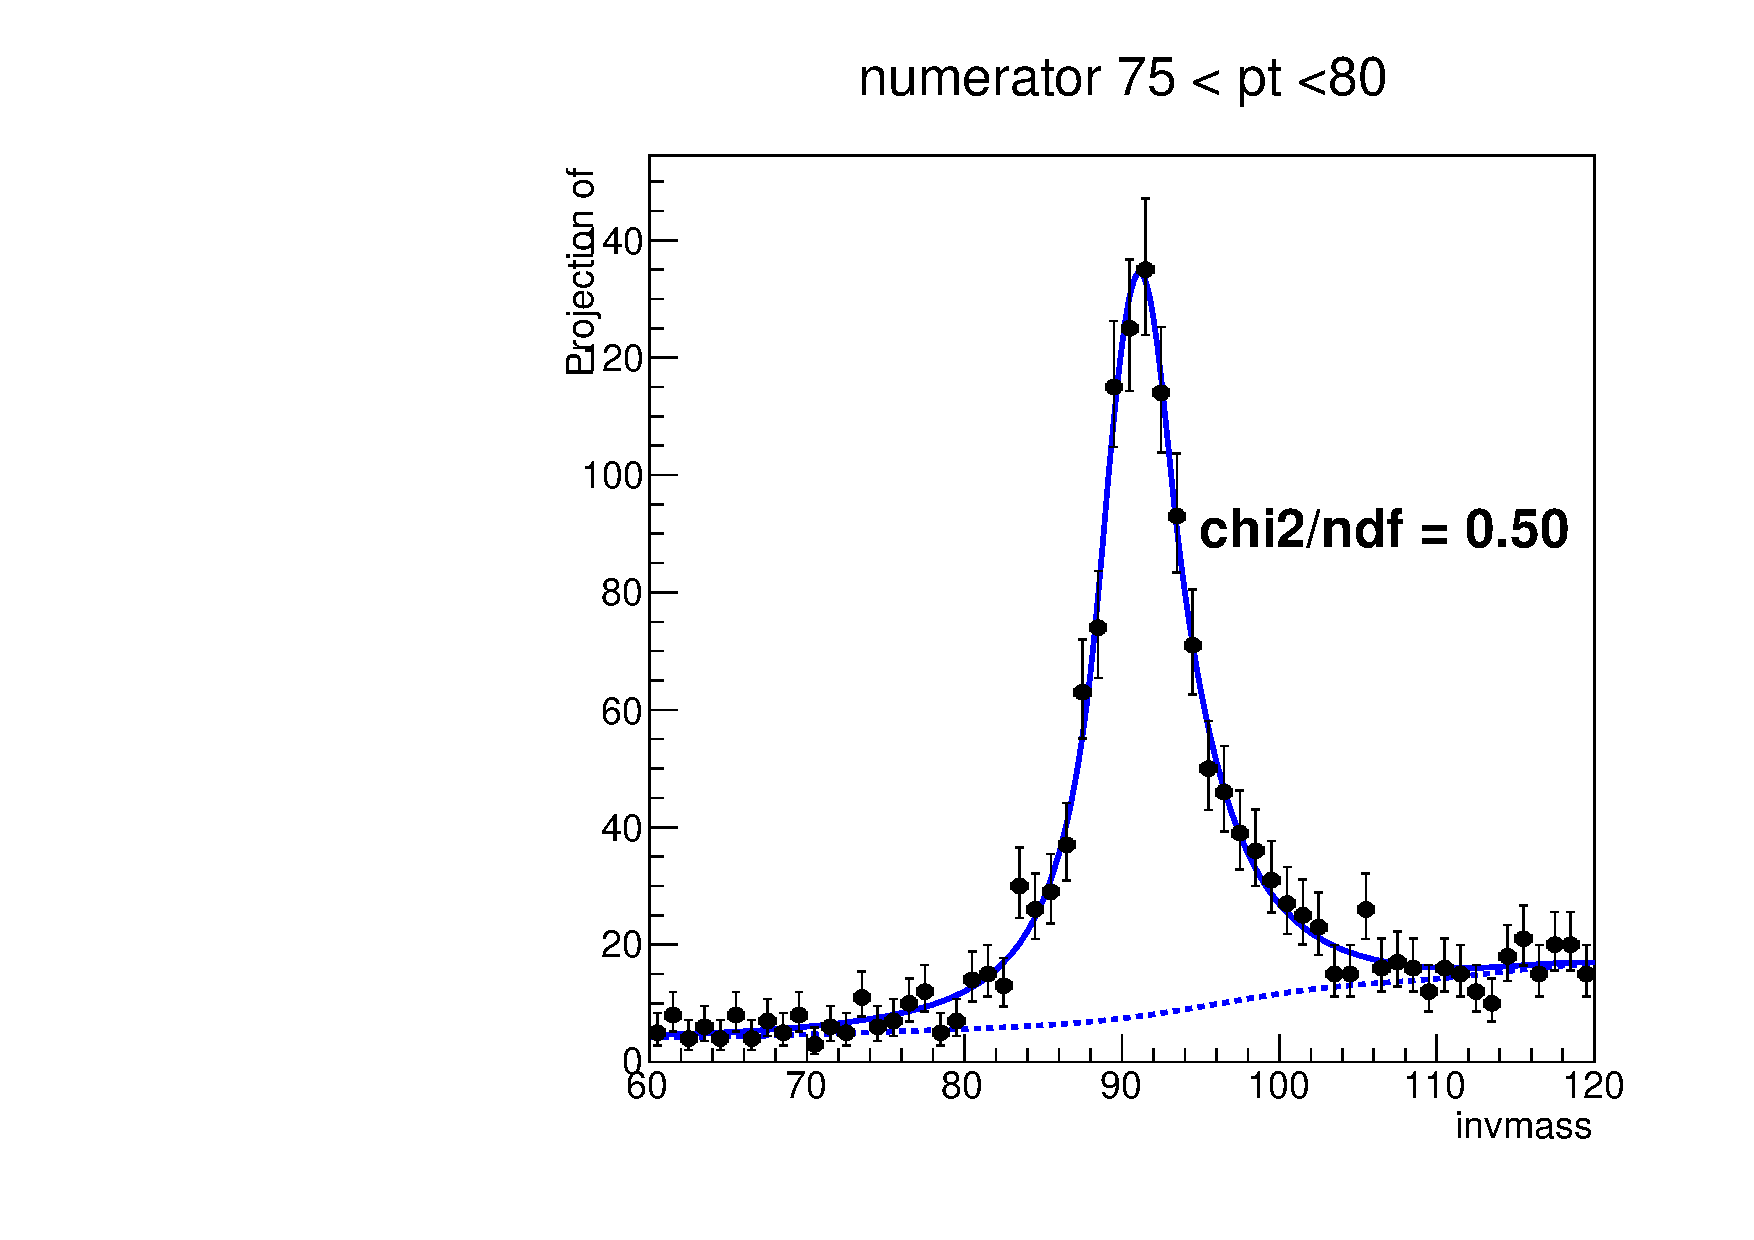
\includegraphics[width=0.24\textwidth]{Figures/Bw_ker_pt_num_75_80.pdf}   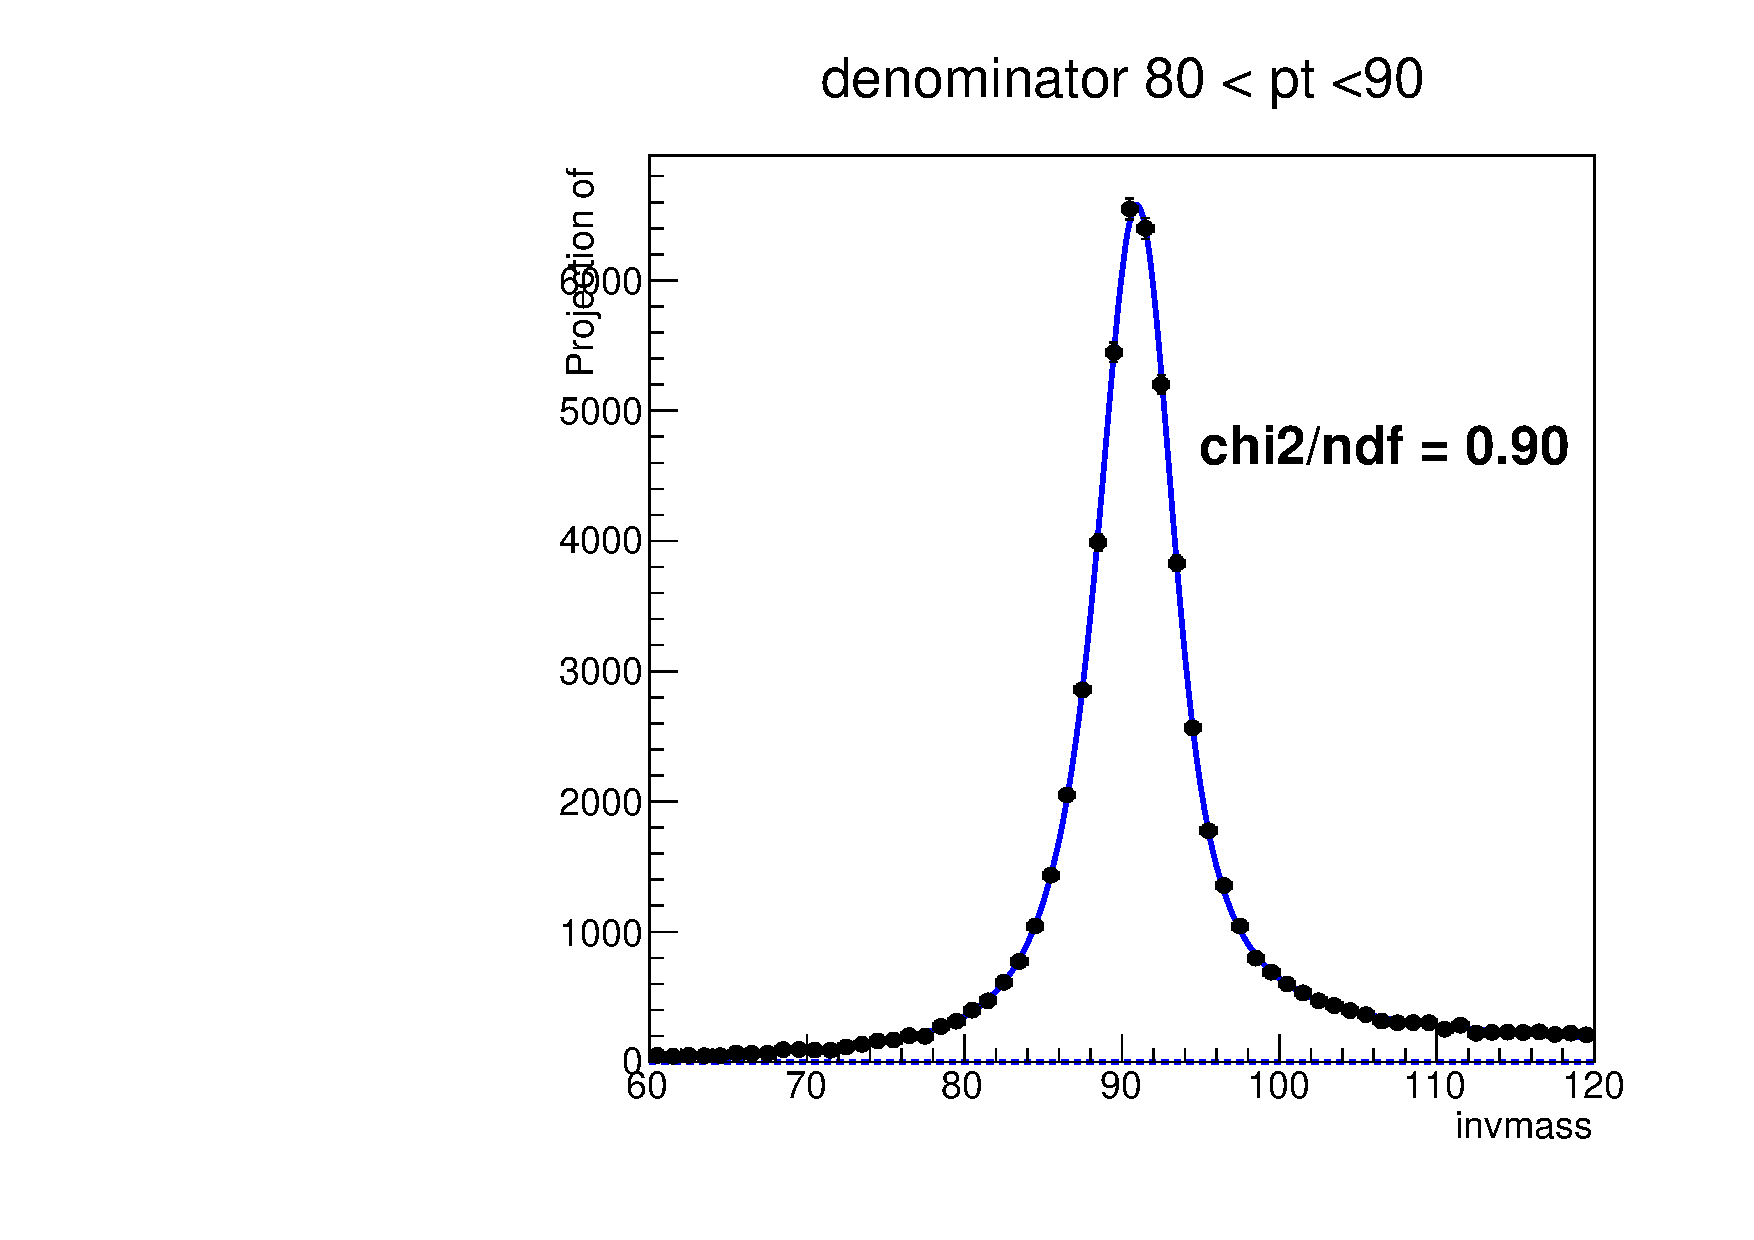
\includegraphics[width=0.24\textwidth]{Figures/Bw_ker_pt_den_80_90.pdf} 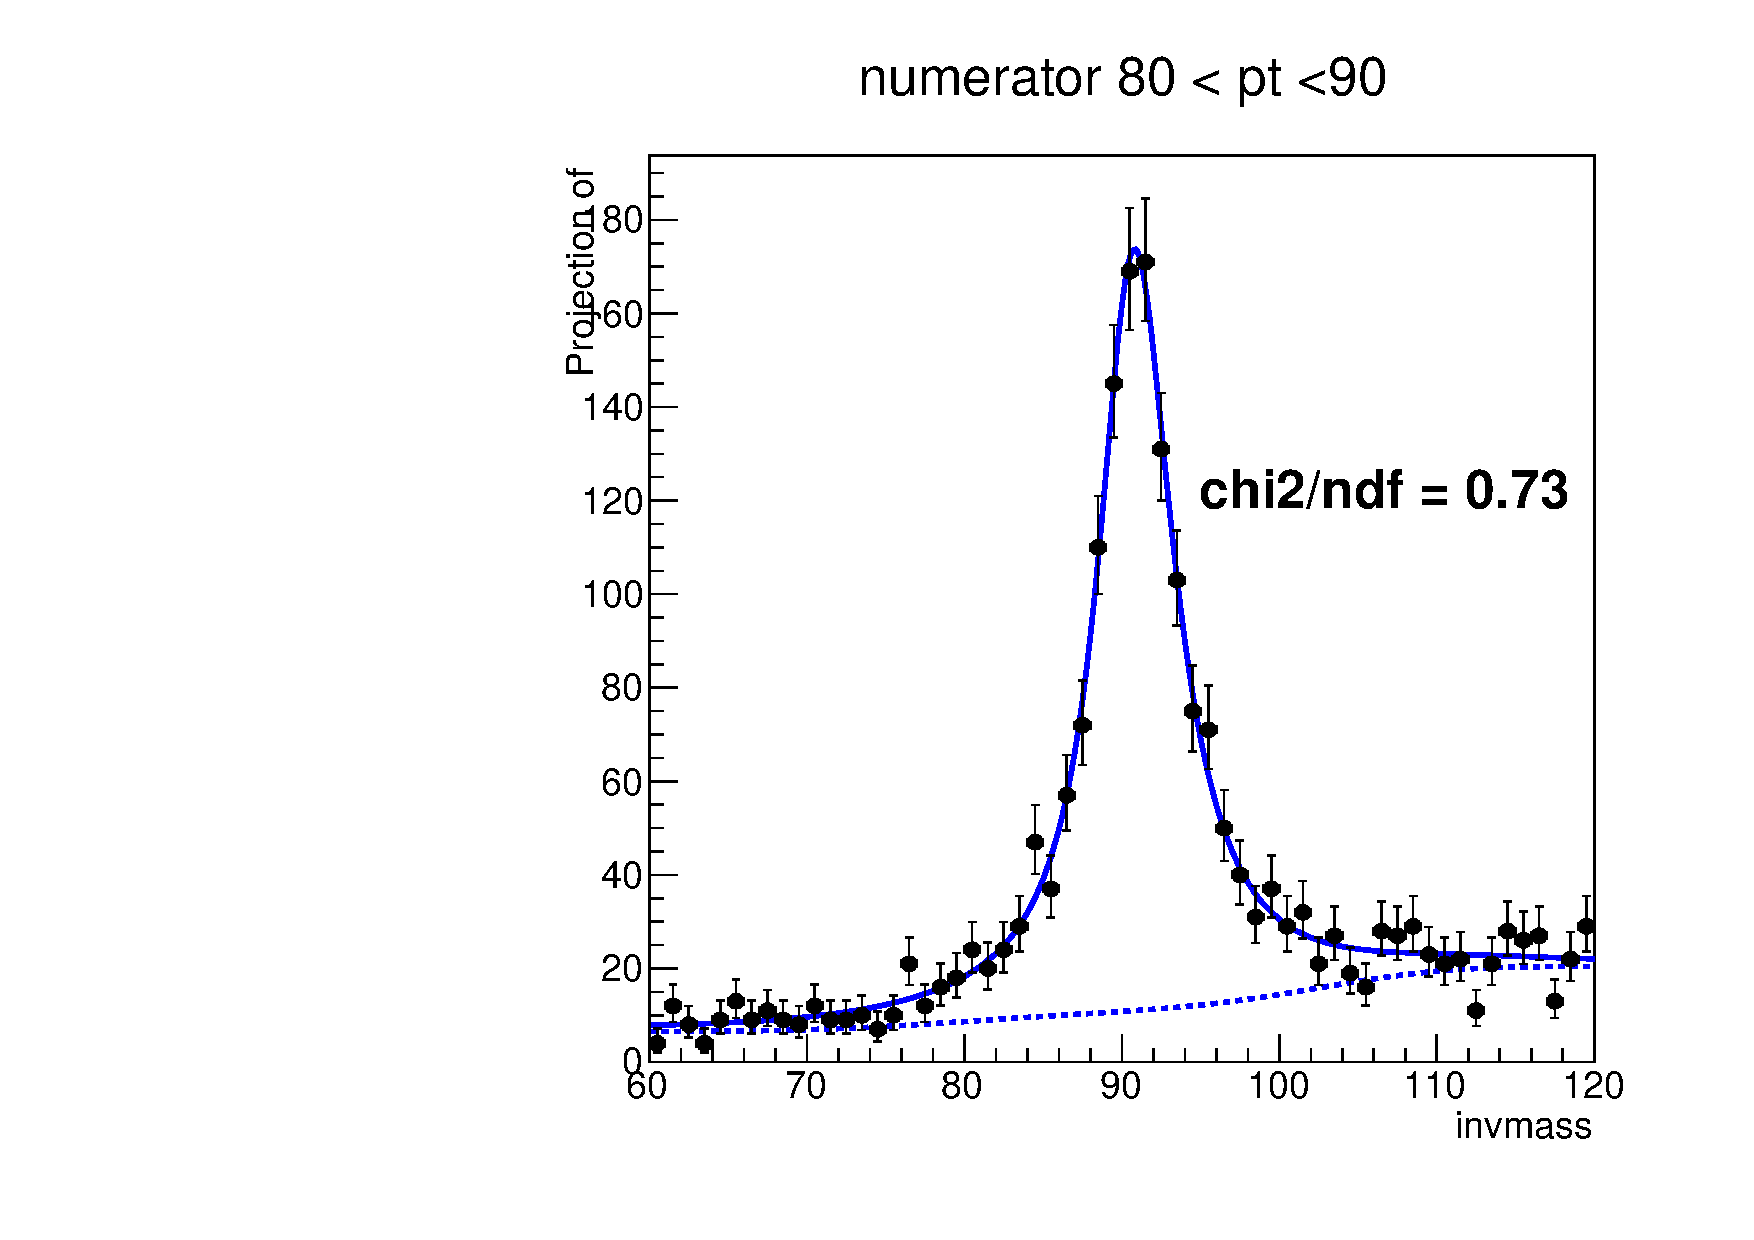
\includegraphics[width=0.24\textwidth]{Figures/Bw_ker_pt_num_80_90.pdf} \\
    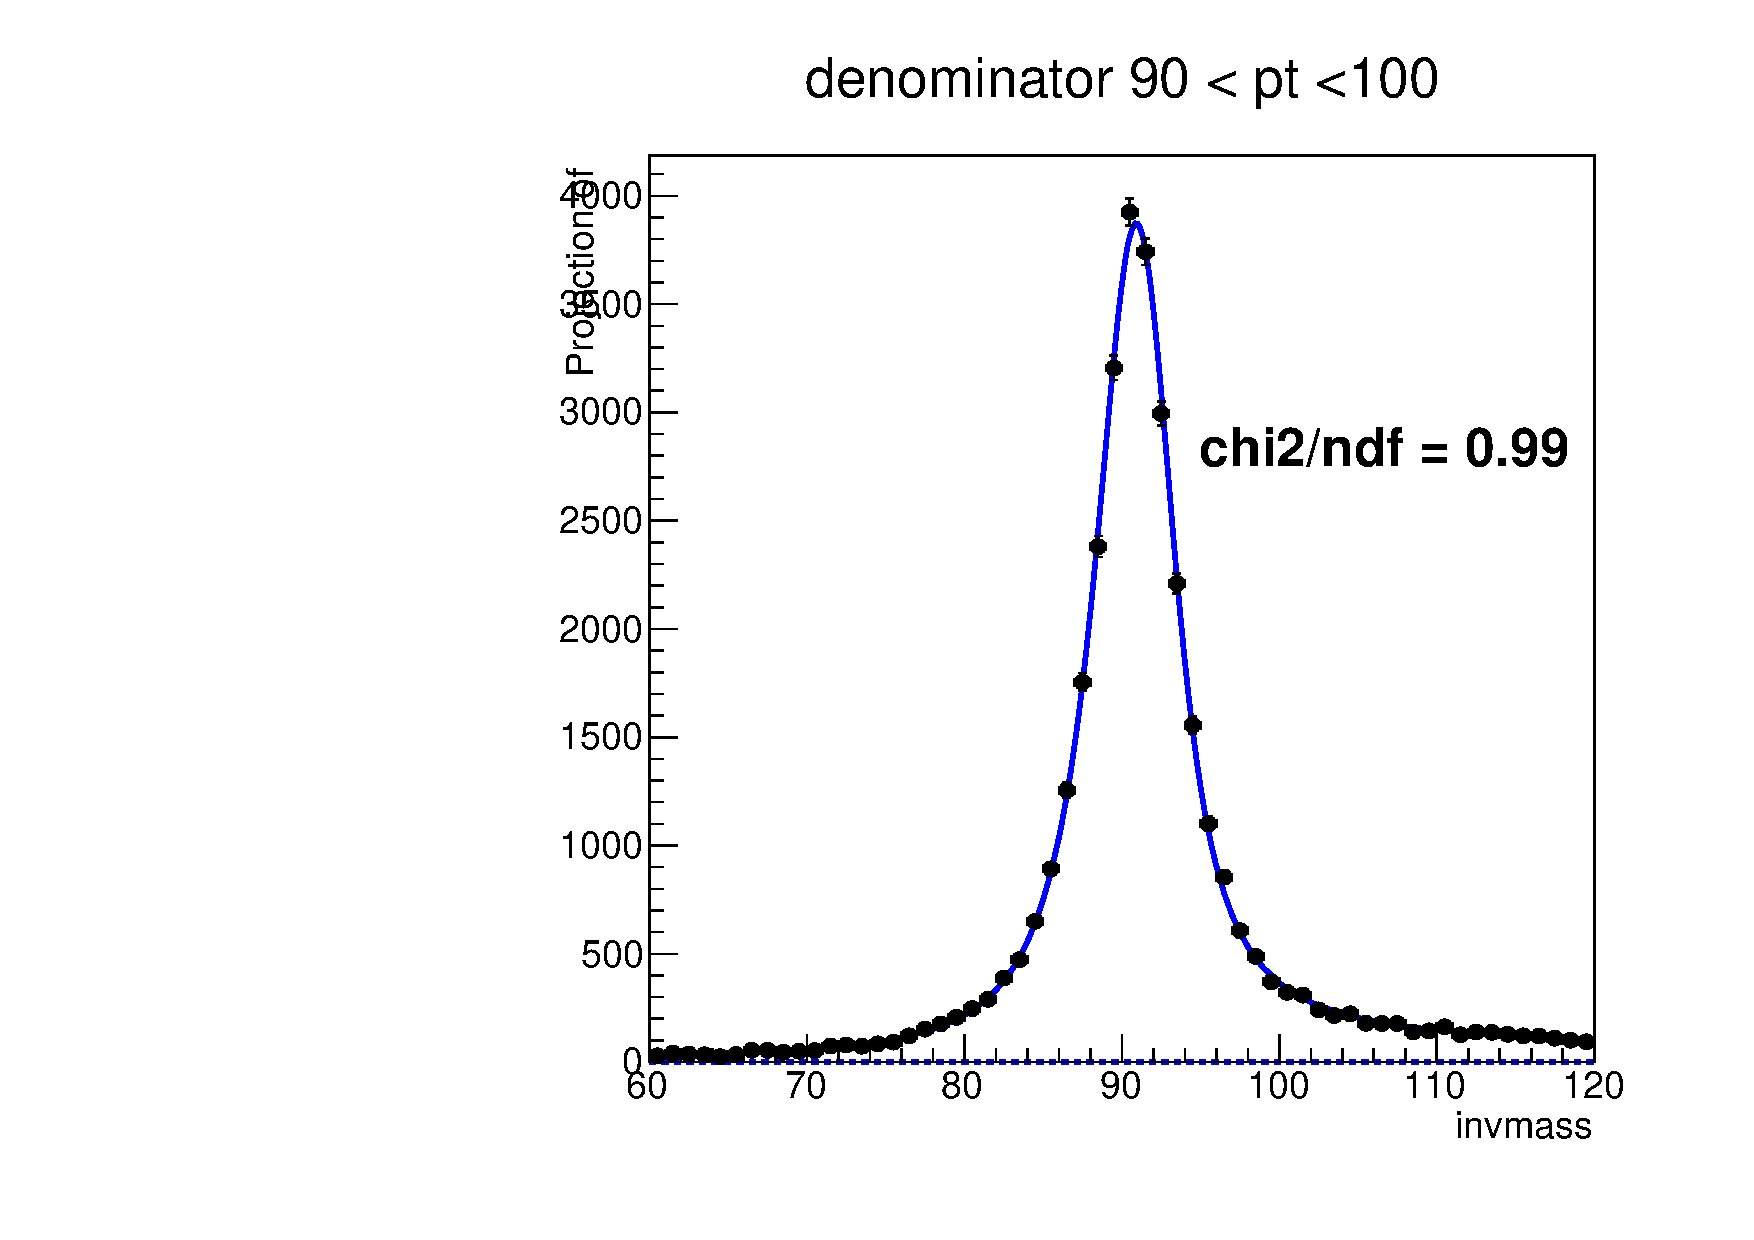
\includegraphics[width=0.24\textwidth]{Figures/Bw_ker_pt_den_90_100.pdf}  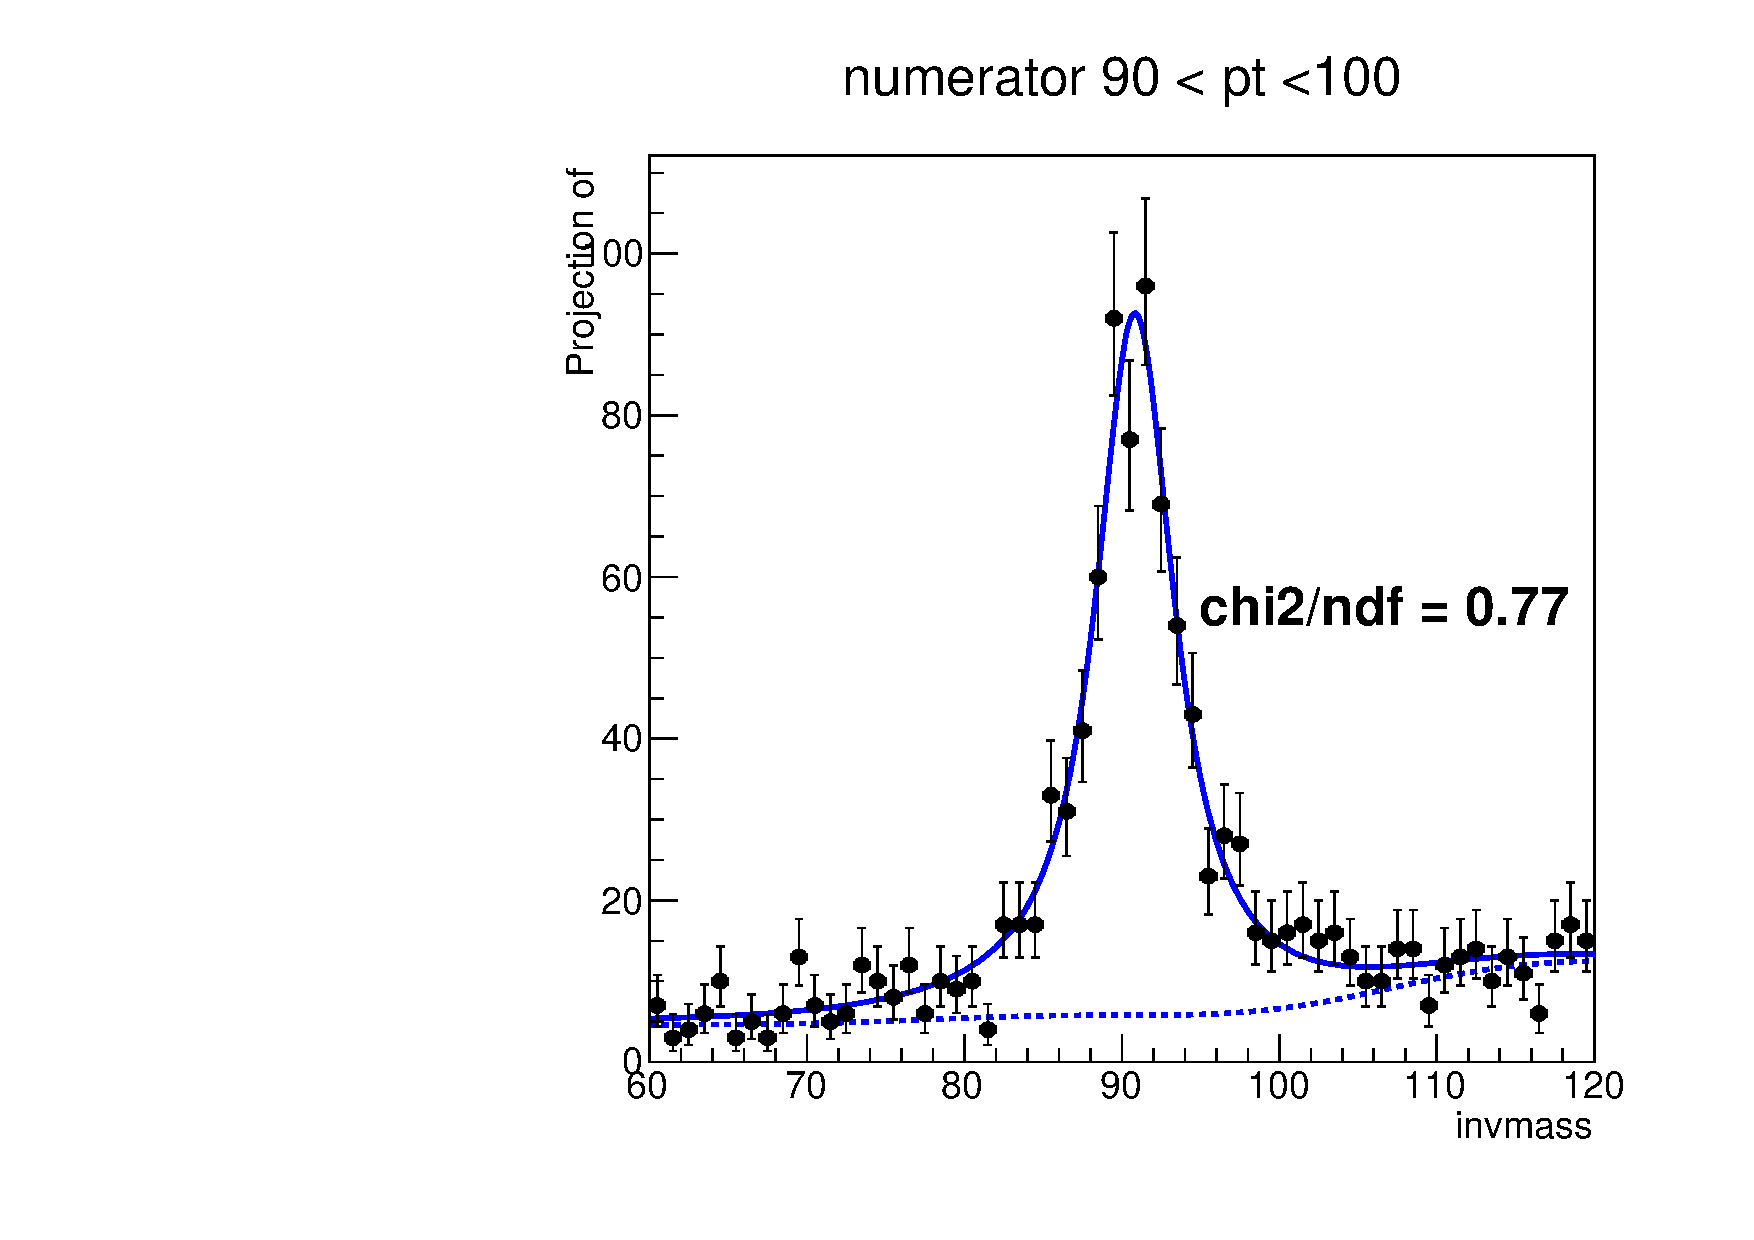
\includegraphics[width=0.24\textwidth]{Figures/Bw_ker_pt_num_90_100.pdf}   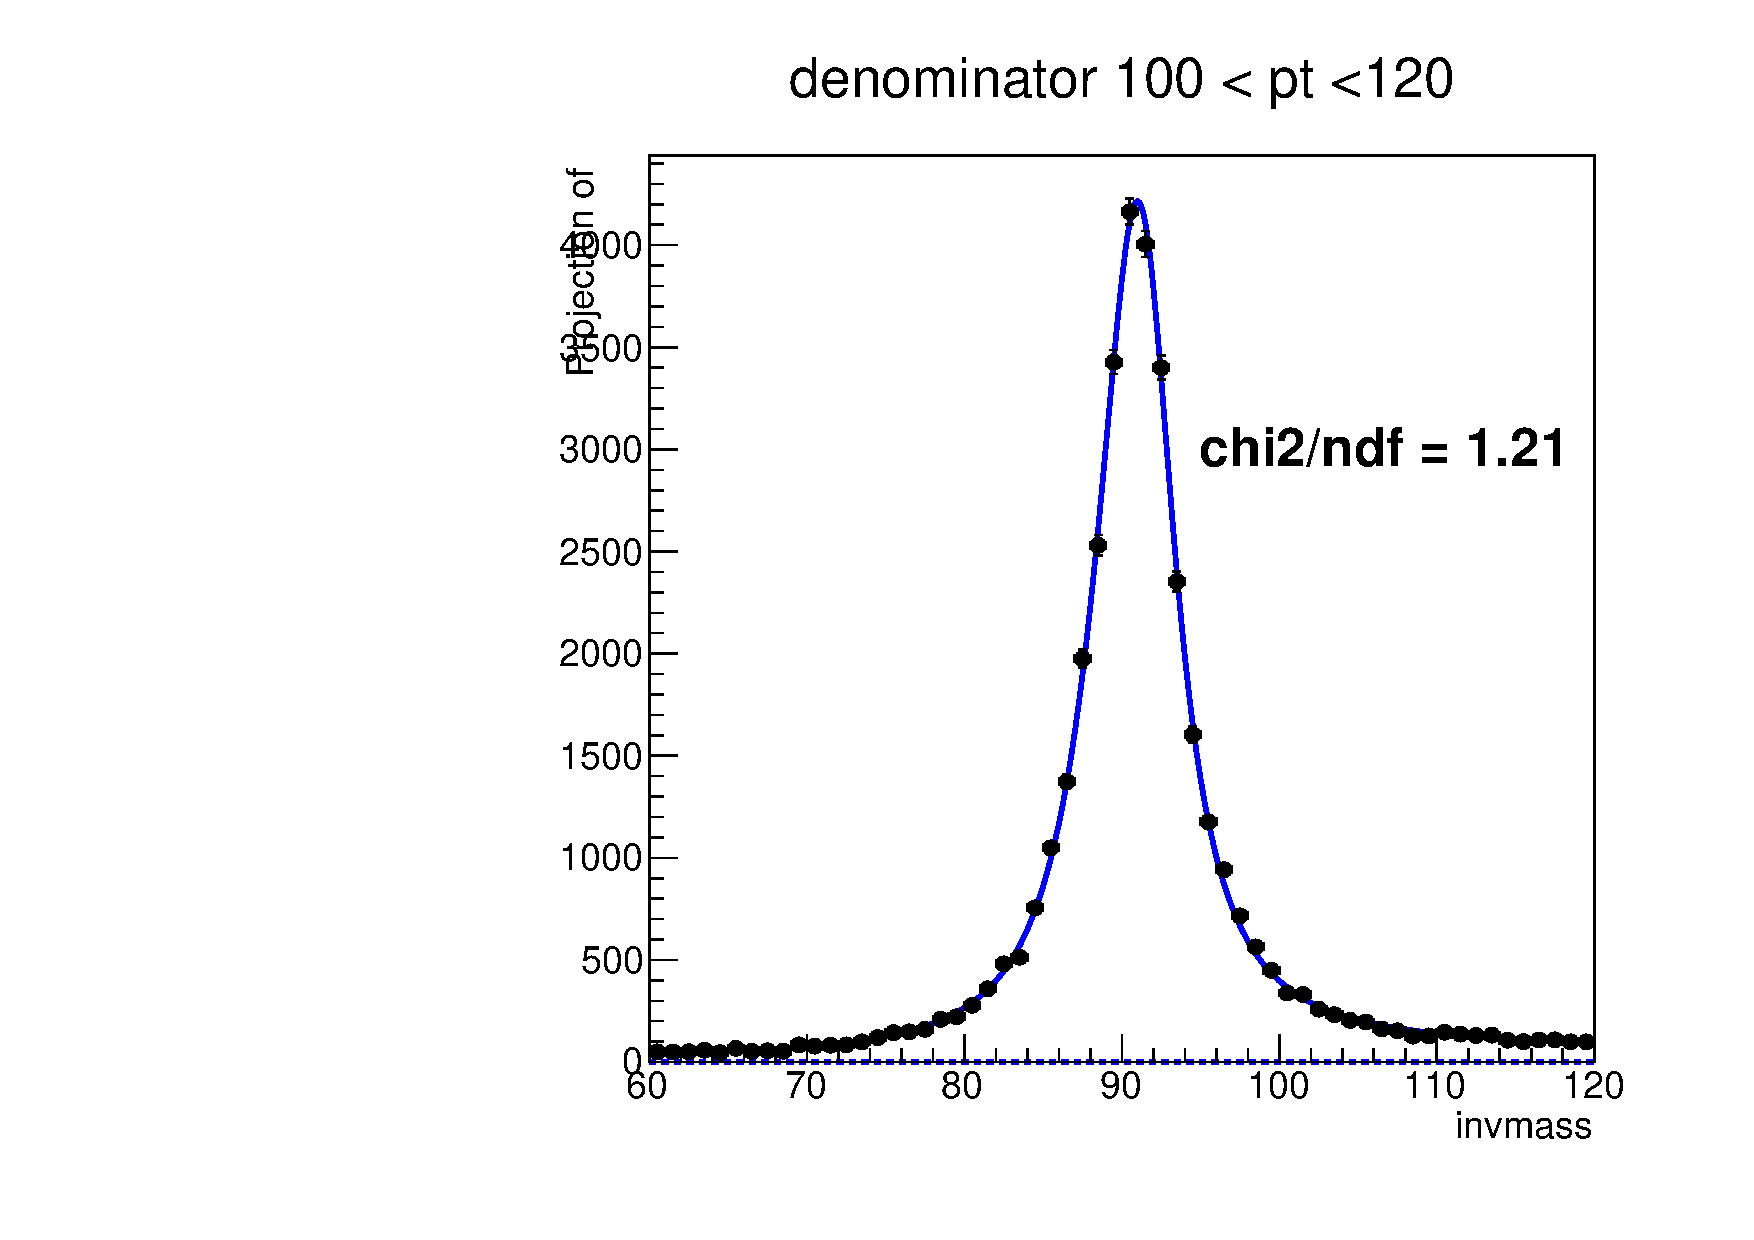
\includegraphics[width=0.24\textwidth]{Figures/Bw_ker_pt_den_100_120.pdf} 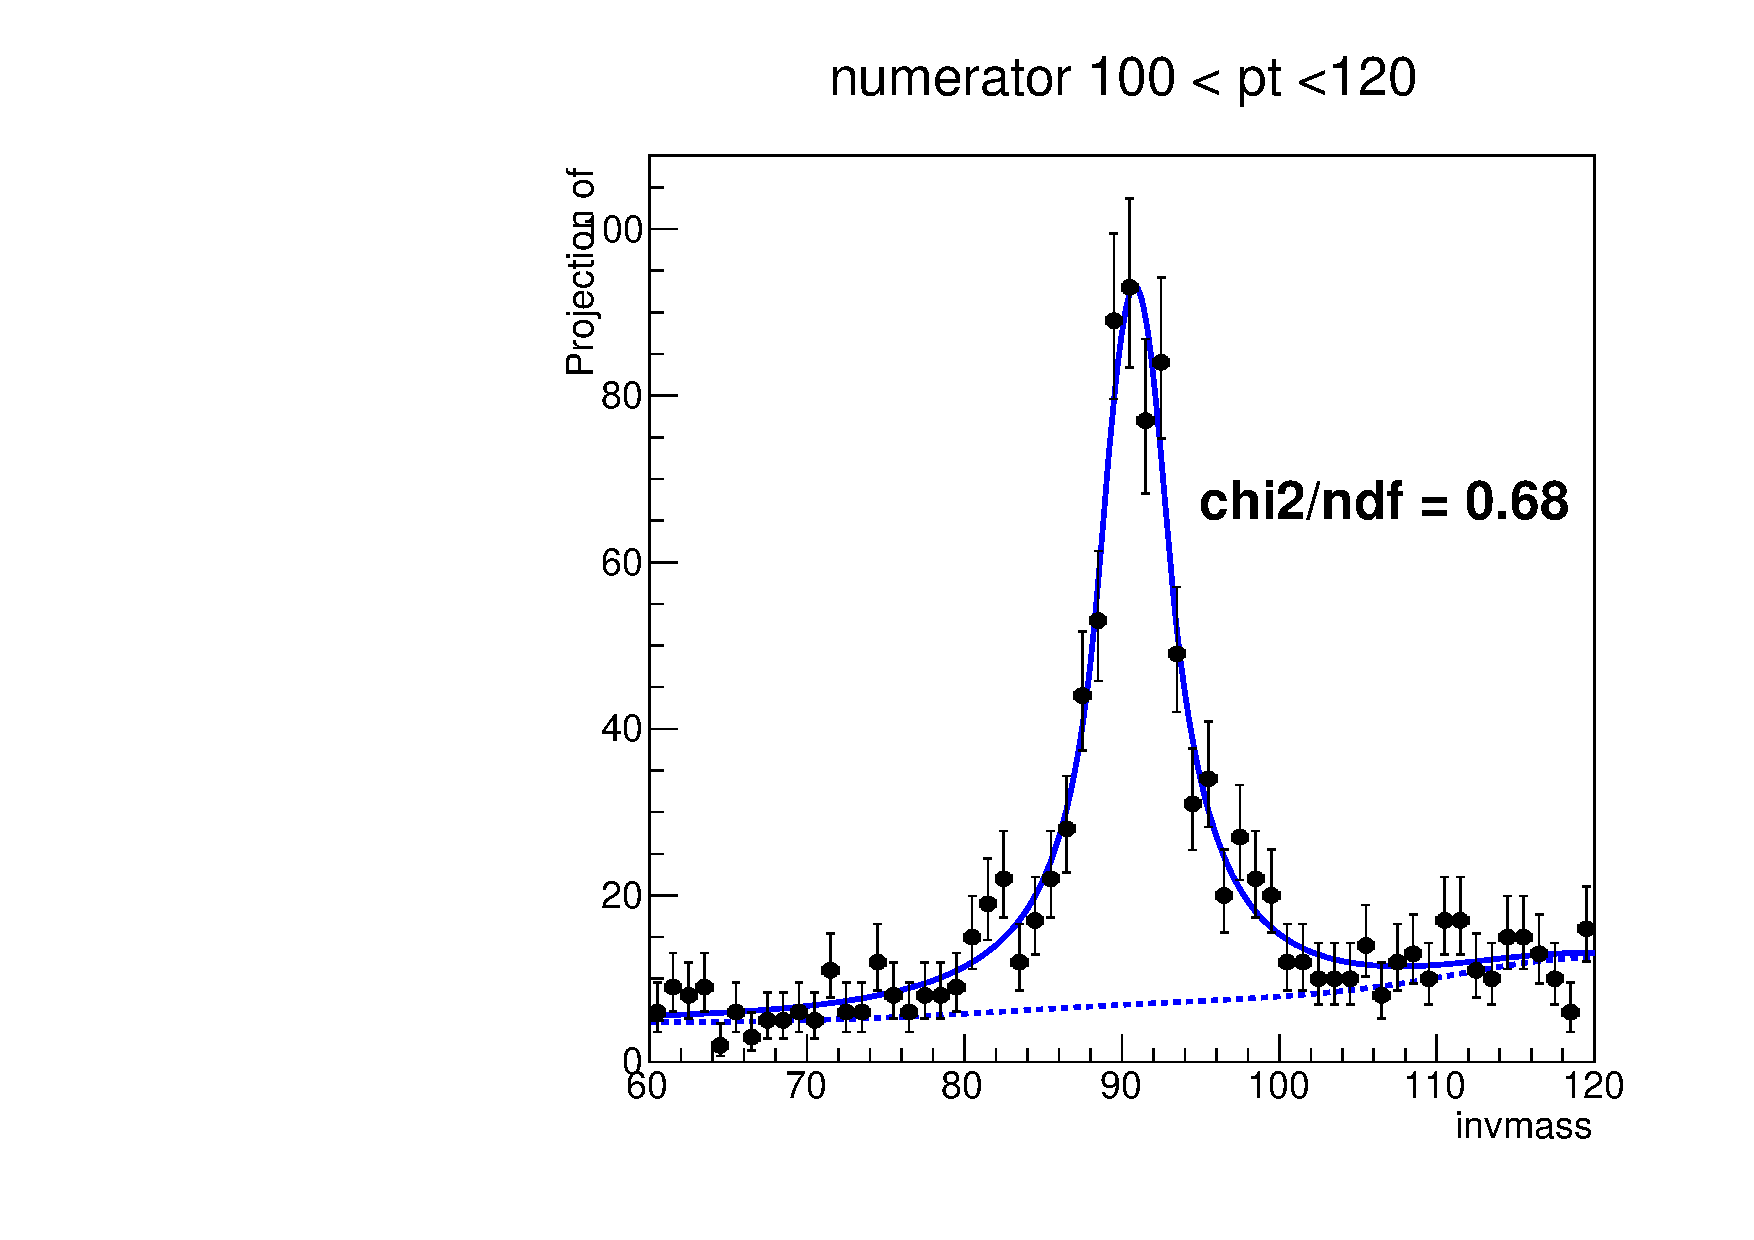
\includegraphics[width=0.24\textwidth]{Figures/Bw_ker_pt_num_100_120.pdf} \\
  \caption{Tag-and-probe fits in various $p_T$ bins for electron misidentification rate measurement. }
 \label{fig:fitAllele}
\end{figure}


Once the normalization and parameters of the signal functions are determined from the fit, the $N^{ee}$ and $N^{e\gamma}$ values are given by the integrals of signal shapes between 80 GeV and 101 GeV in the corresponding samples. The global fake rate for electrons with $p_T >$ 30 GeV is \\
\begin{equation}
        f = (2.29 \pm 0.14)\%
\end{equation}\\

The electron misidentification rate measured in Z decay events will be applied to estimate the number and shape of fake photons in signal region. However, the kinematic distributions of signal photon candidates may differ from the ones from Z decay, and result in a different fake rates. To correctly extrapolate the misidentification rate to signal region, we considered its dependence on the following three variables: transverse momentum of probe ($p_T$); the pseudo rapidity of the probe ($\eta$); and the number of vertices in the event ($N_{vtx}$). The chosen of $p_T$ and $\eta$ is motivated by the tracker efficiency dependence on these two variables. $N_{vtx}$, on the other hand, is used to model the pileup effect. These dependencies are shown in Figure \ref{fig:elefakepho_rate_pt}.


\begin{figure}
  \centering
    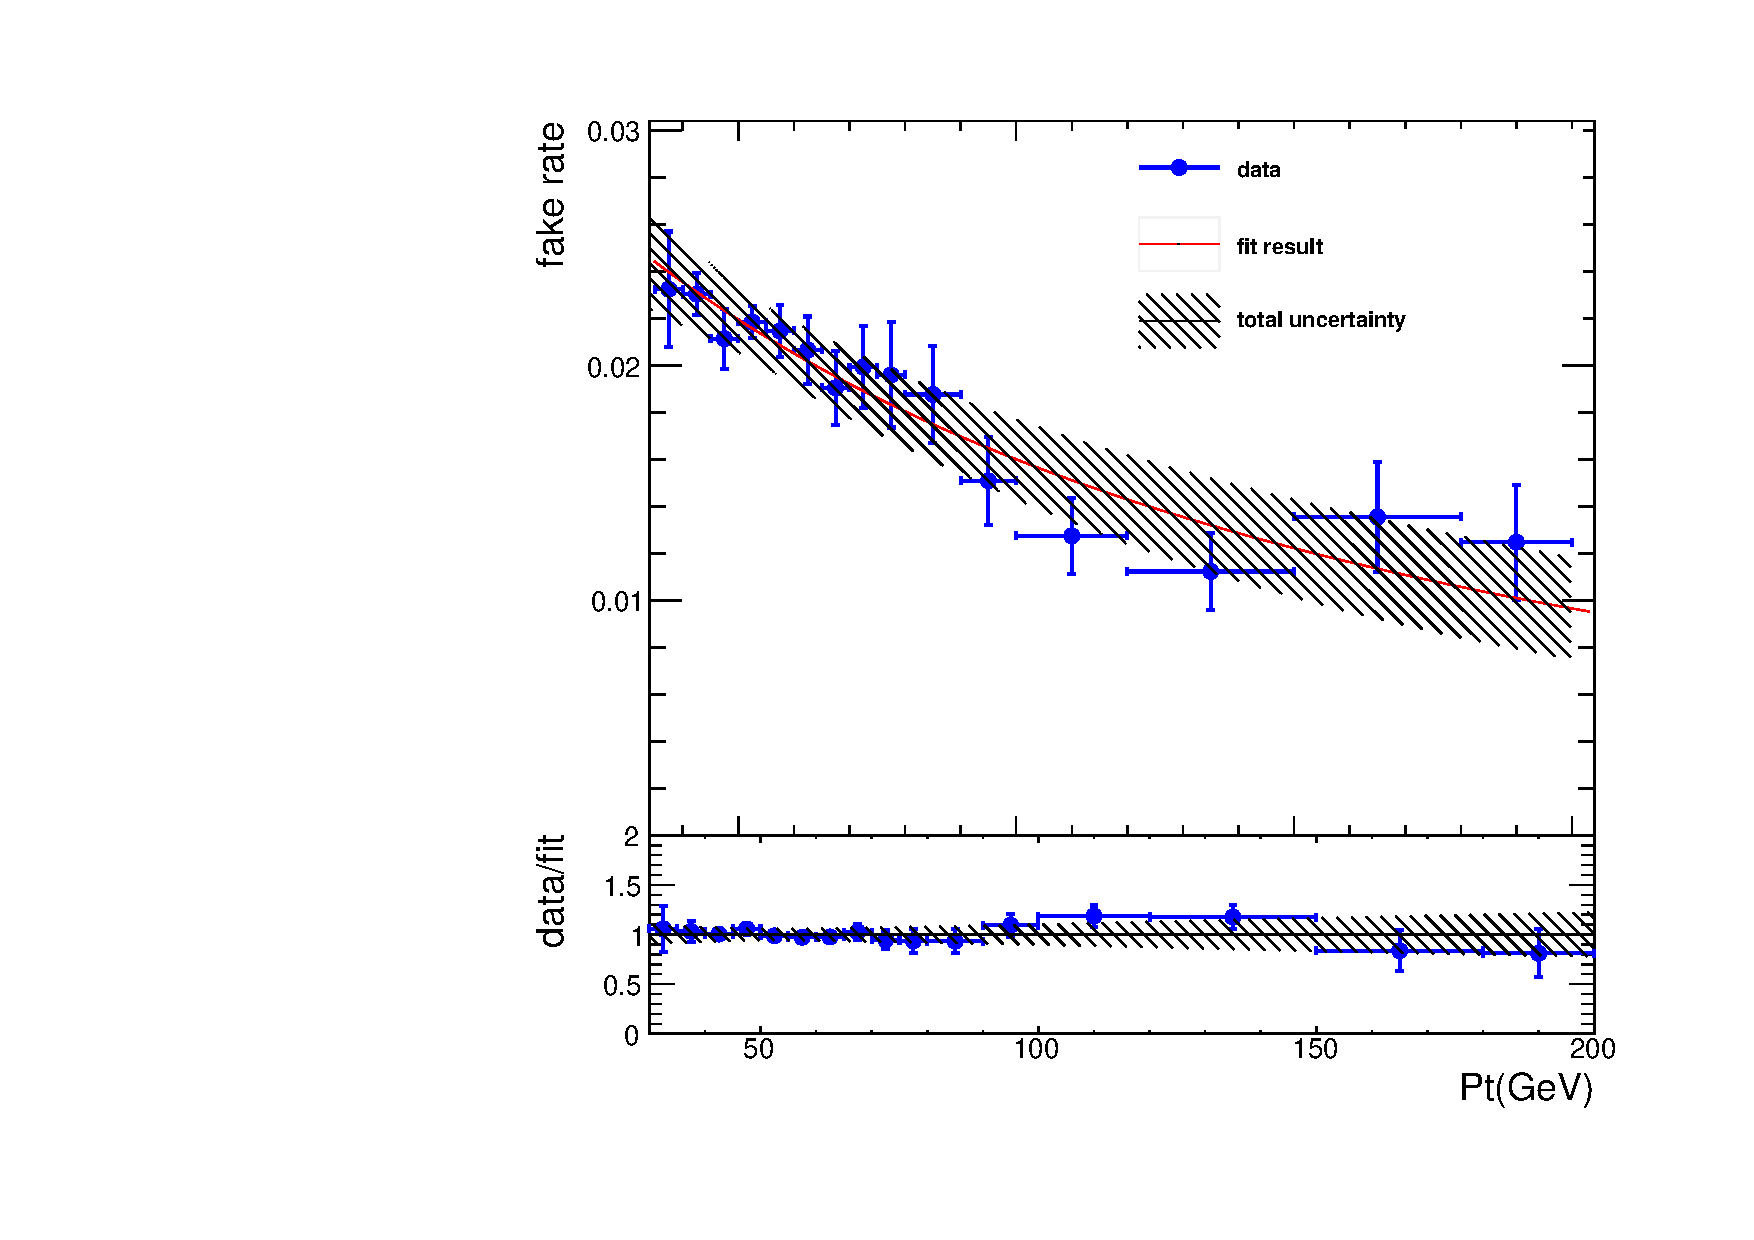
\includegraphics[width=0.45\textwidth]{Figures/elefake_pt_systematic_data.pdf}
    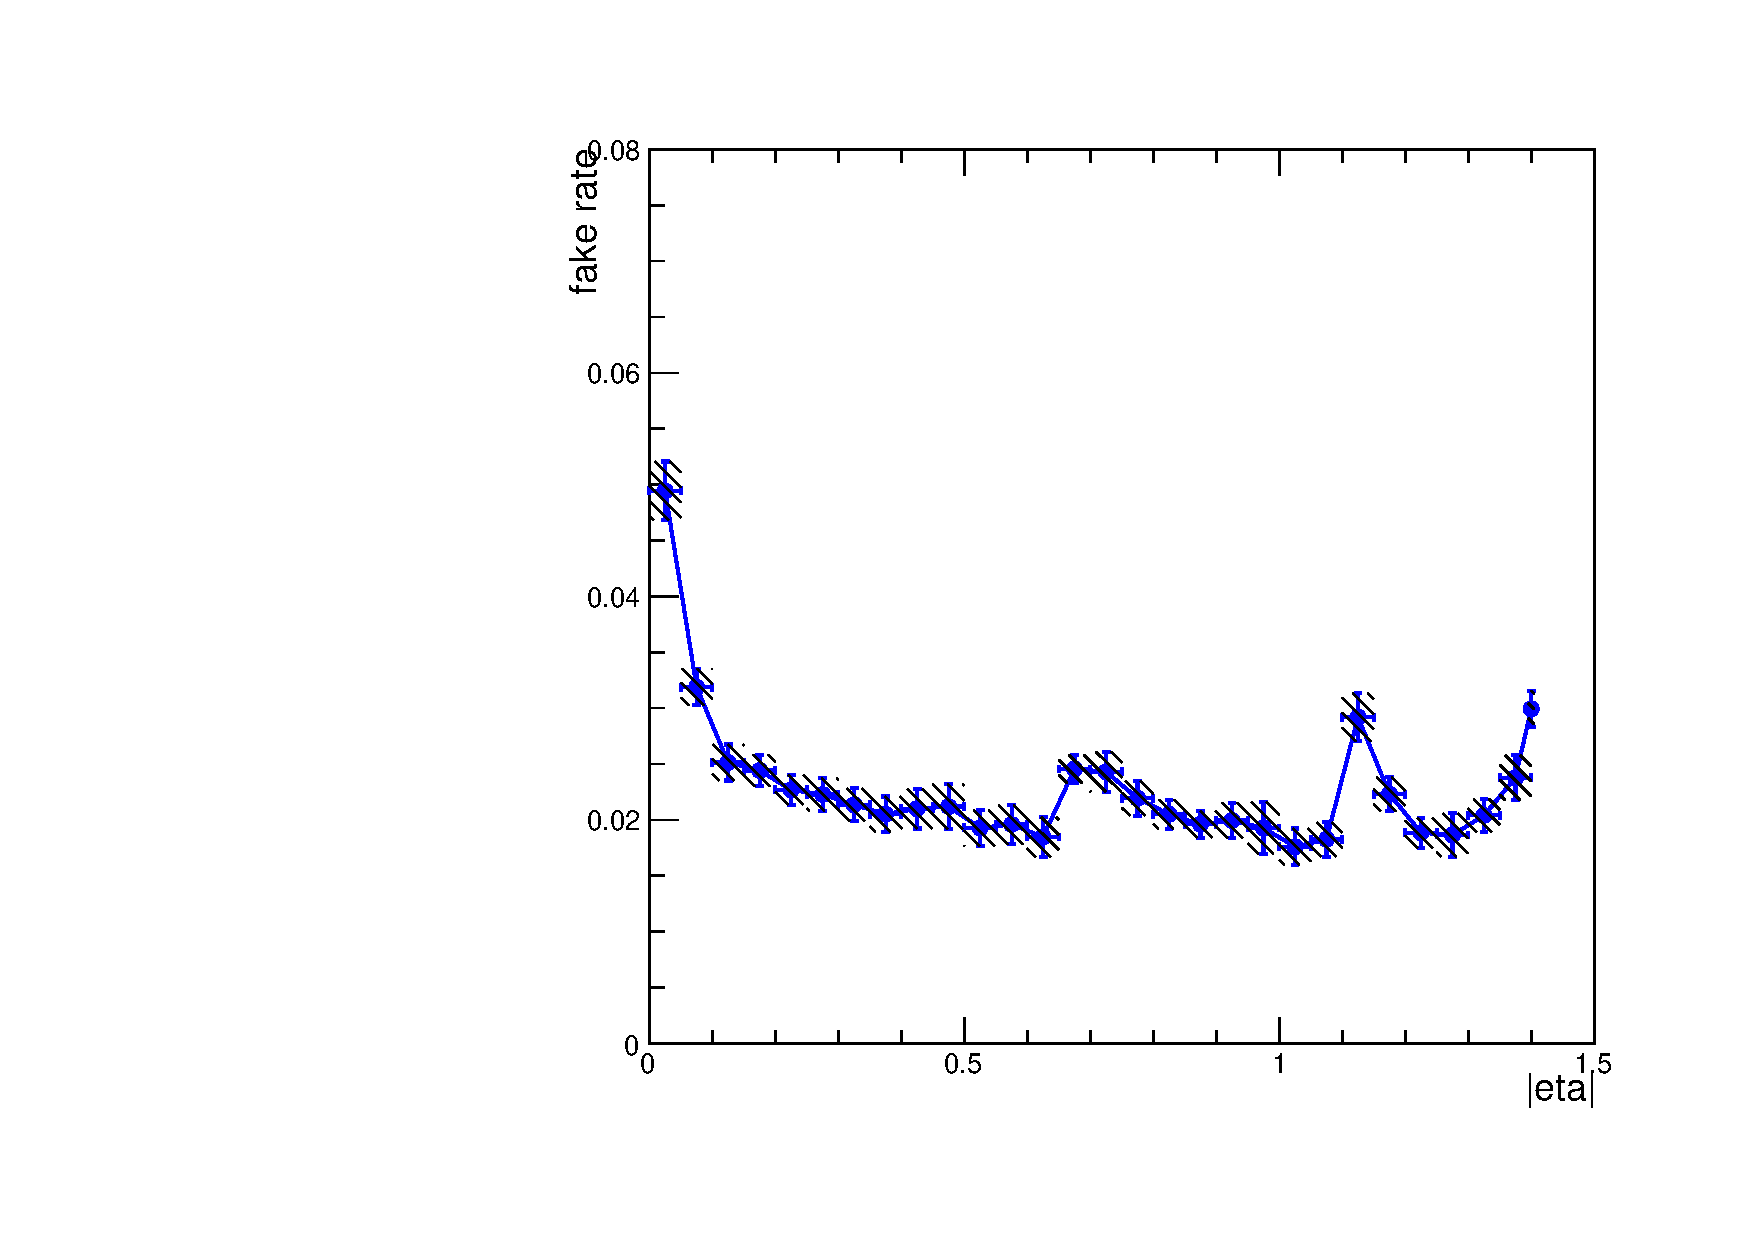
\includegraphics[width=0.45\textwidth]{Figures/elefake_eta_systematic_data.pdf}
     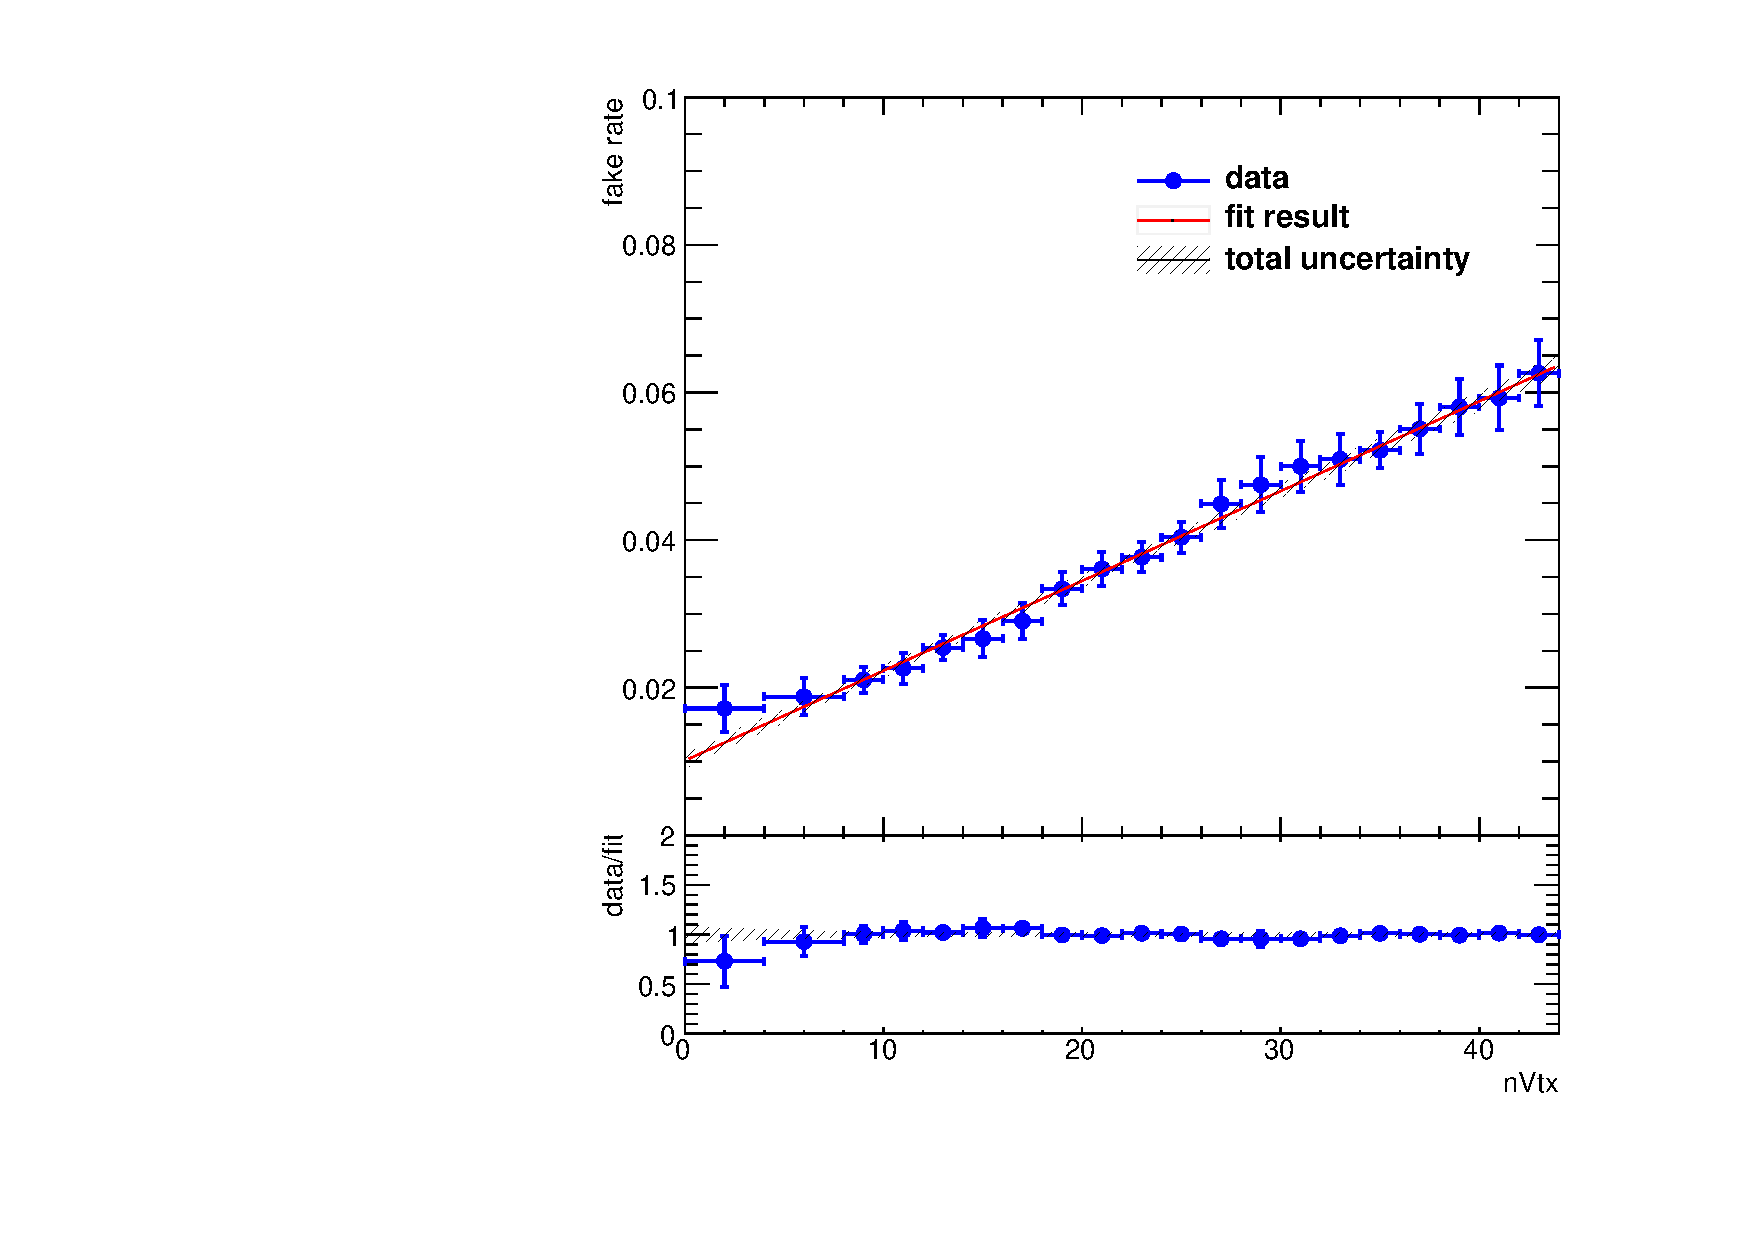
\includegraphics[width=0.5\textwidth]{Figures/elefake_vtx_systematic.pdf}
  \caption{The electron misidentification rate as a function of $p_T$ (top left), $\eta$ (top right) and $N_{vtx}$ (bottom), along with the systematic uncertainties.}
  \label{fig:elefakepho_rate_pt}
\end{figure}

The dependencies of the misidentification rate on $p_T$ and $N_{vtx}$ can be described by parametrized functions. By studying the fake rate in simulations, we determined that the functional forms \\
\begin{eqnarray*}
	f(p_{T})   &=& ( a + b\cdot p_T)^{-\alpha} \\
	f(N_{vtx}) &=& c + \beta \cdot N_{vtx}
\end{eqnarray*}\\
can be used to model the fake rate dependencies on these two variables. The parameters obtained by fitting the functions to fake rate distributions are \\
\begin{eqnarray*}
	a   &=& 6.4 \pm 0.8  \\
	b   &=& (2.9 \pm 0.8) \cdot 10^{-2} \\
	\alpha &=& -1.8 \pm 0.1 \\
	c &=& (5.9 \pm 1.1) \cdot 10^{-3} \\
	\beta &=& (9.2 \pm 0.4) \cdot 10^{-4} \\
\end{eqnarray*}\\

 Assuming that the fake rate depends on each variable independently, the combined fake rate can be expressed as function of ($p_T$, $\eta$, $N_{vtx}$) with the following form 
\begin{equation} 
	f(p_{T}, \eta, N_{vtx}) = N \cdot f(p_T) \cdot f(N_{vtx}) \cdot f(\eta)
\end{equation}

where N is a constant, and f($\eta$) is the dependence of pseudo rapidity, whose value is given by the fake rate of the corresponding $\eta$ bin. 

To fix the constant N, we applied the misidentification rate to the denominator sample and require the predicted number of fake photons to be the same as $N^{e\gamma}$. The resulting N value is: \\
\begin{equation} 
	N = (1.83 \pm 0.11) \cdot 10^{3}
\end{equation}


The electron-fake-photon rate calculated above is applied to the electron-enriched proxy sample to predict the contribution from misidentified electrons. Uncertainties of the misidentified electron background are evaluated with toy Monti-Carlo experiments. First, the parameters of the fake rate functions are pulled from a multi-variant Gaussian distribution with means given by the nominal fitting result, and covariance matrix given by the fitting errors. The ranges of the pulled parameters are restricted to be one sigma around the nominal values. The normalization factor N is recalculated using the new parameters. The toy MC is generated 1000 times to obtain distributions of the background variations. The one sigma band is constructed using the toy results.\\

   This background estimation method is tested on simulated DY, WW, WZ and $t\bar{t}$ events. The misidentification rate derived from the DY samples using tag and probe method is compared to the true fake rate calculated by truth-matching the photons to generated electrons, and their difference are considered as a source of systematic uncertainty. The proxy events selected from the mixed simulation samples are scaled by the misidentification rate to predict the number of fake photons in the samples. As shown in Figure \ref{fig:efakephoclosure_egamma} and Figure \ref{fig:efakephoclosure_mg}, the predicted distributions show good agreement with the real misidentified electrons.  

\begin{figure}
  \centering
    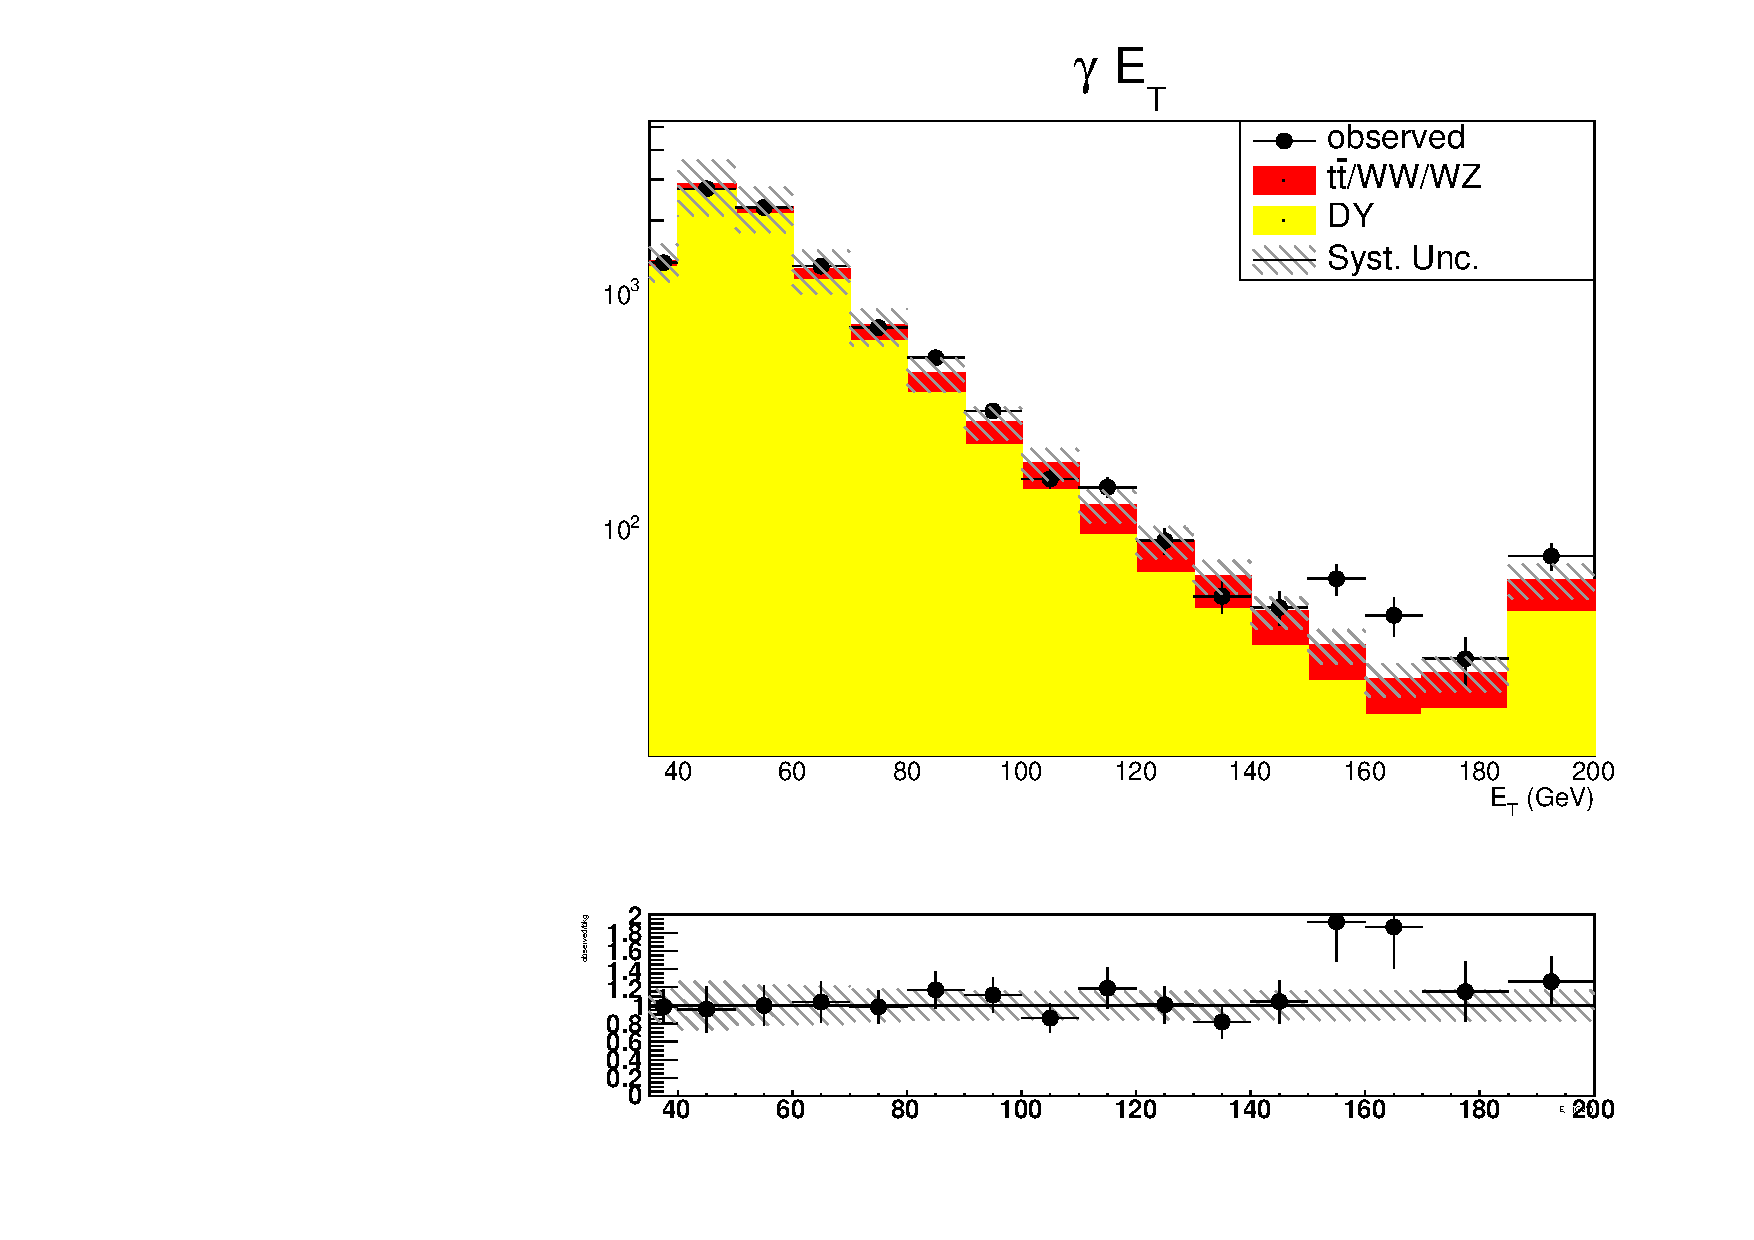
\includegraphics[width=0.45\textwidth]{Figures/closure_elefakepho_PhotonEt_egamma.pdf}
    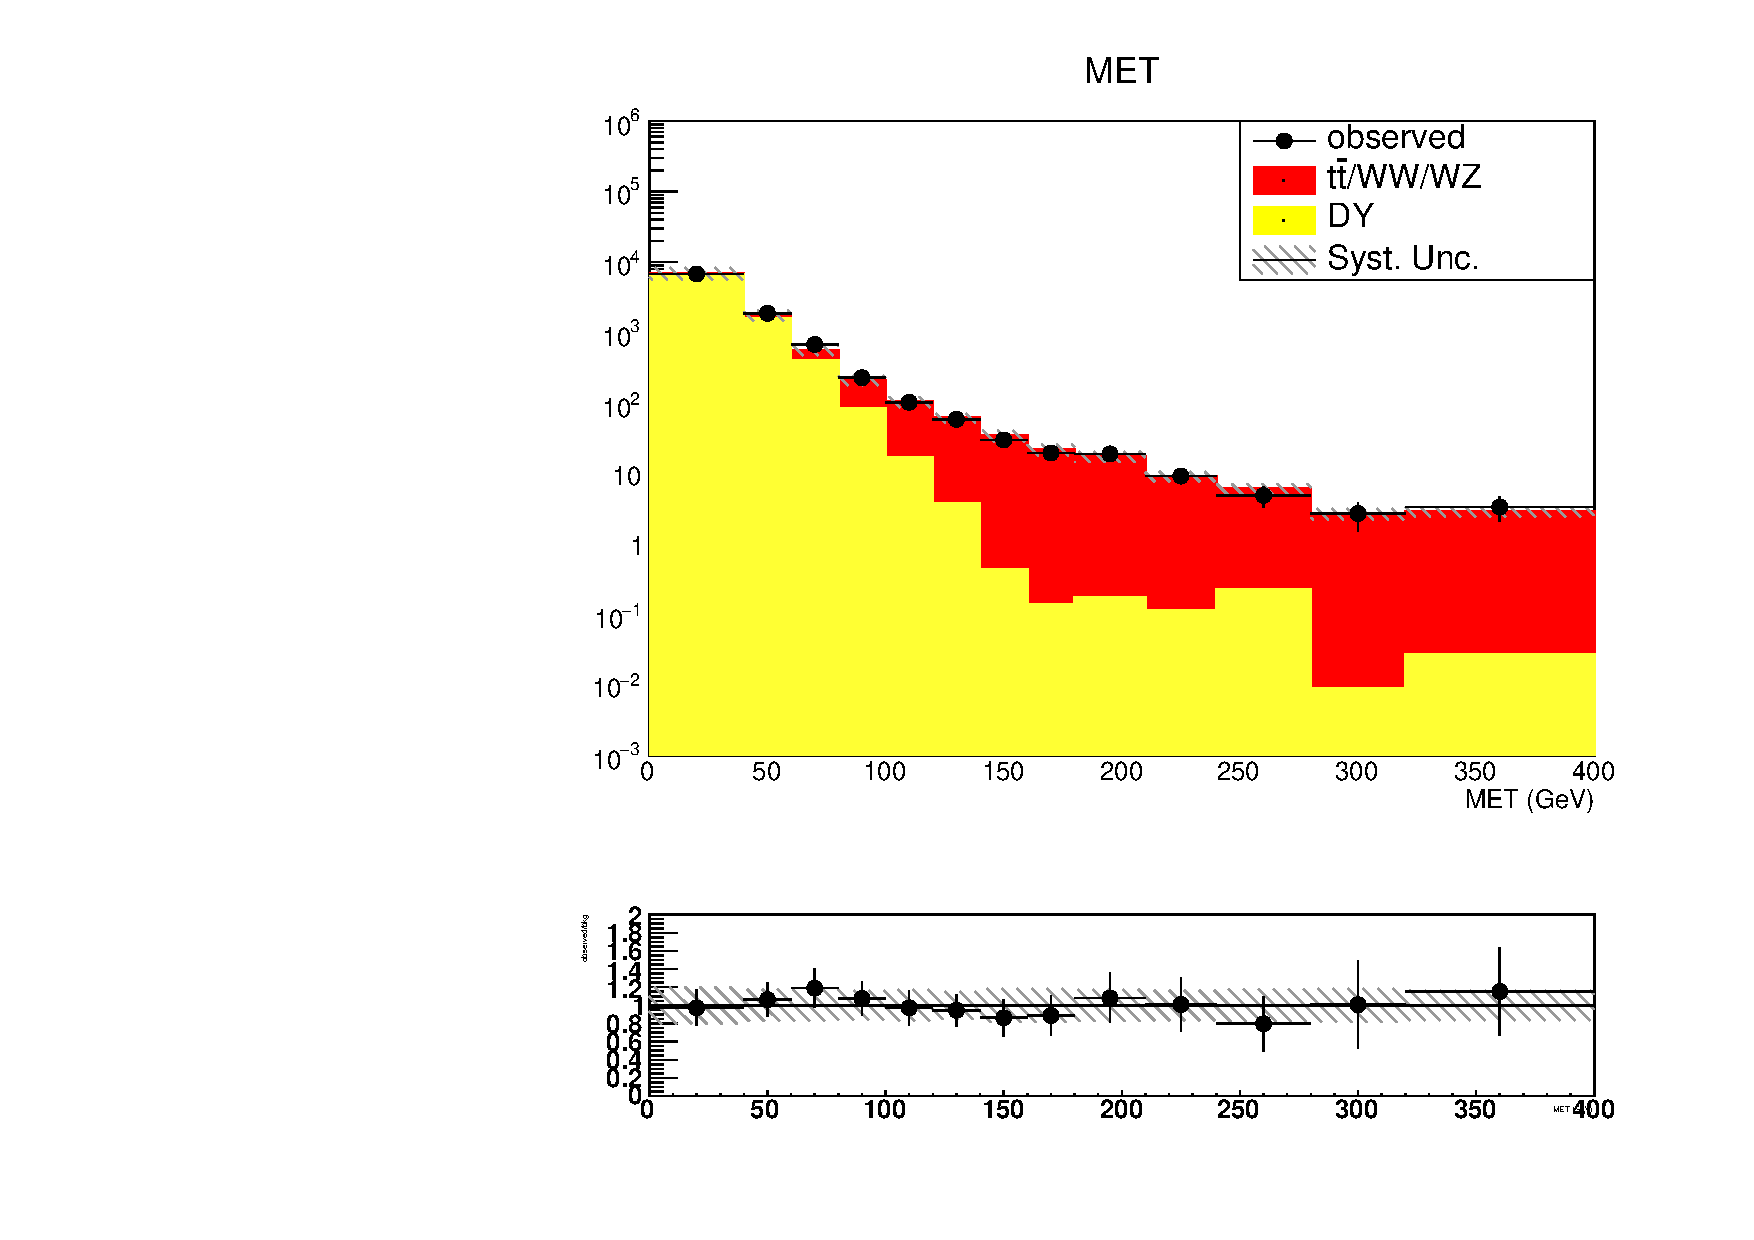
\includegraphics[width=0.45\textwidth]{Figures/closure_elefakepho_MET_egamma.pdf}
    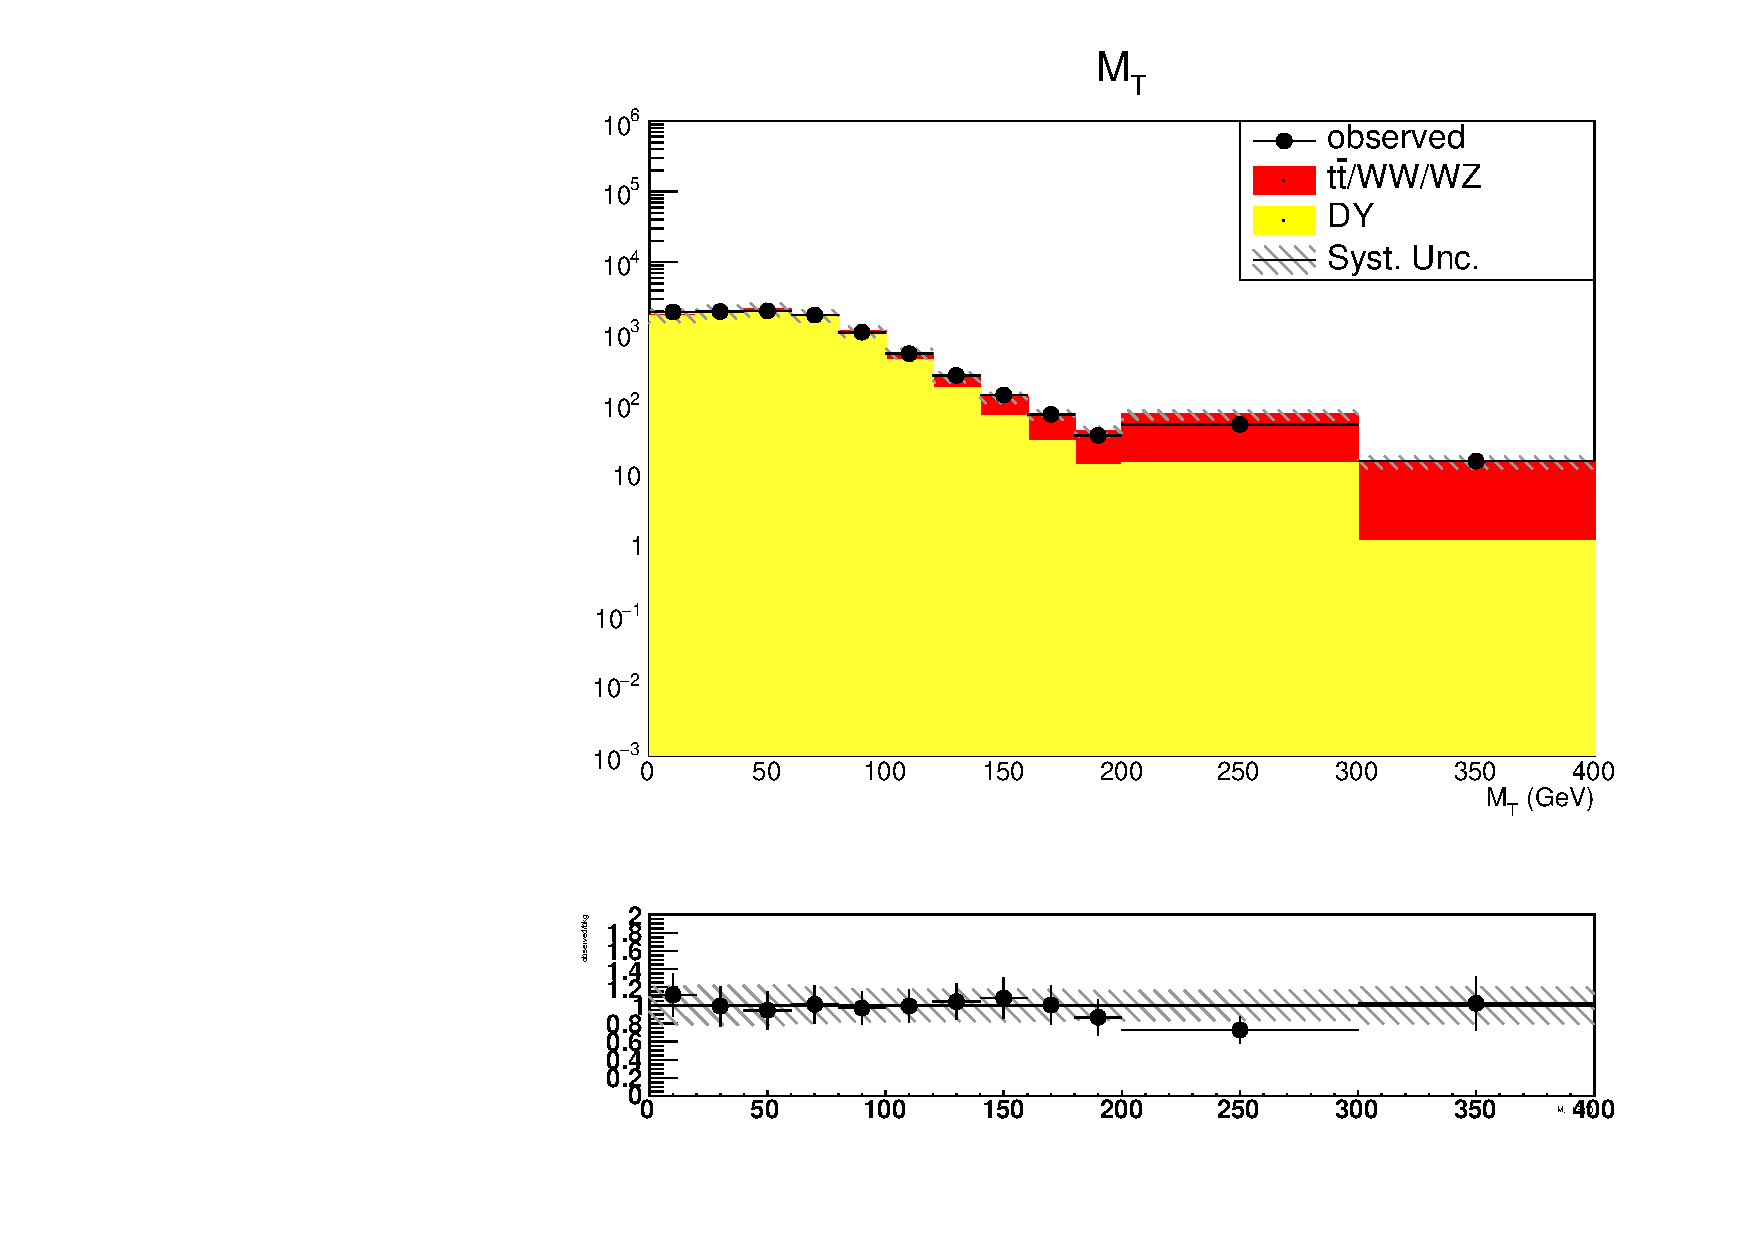
\includegraphics[width=0.45\textwidth]{Figures/closure_elefakepho_MT_egamma.pdf}
    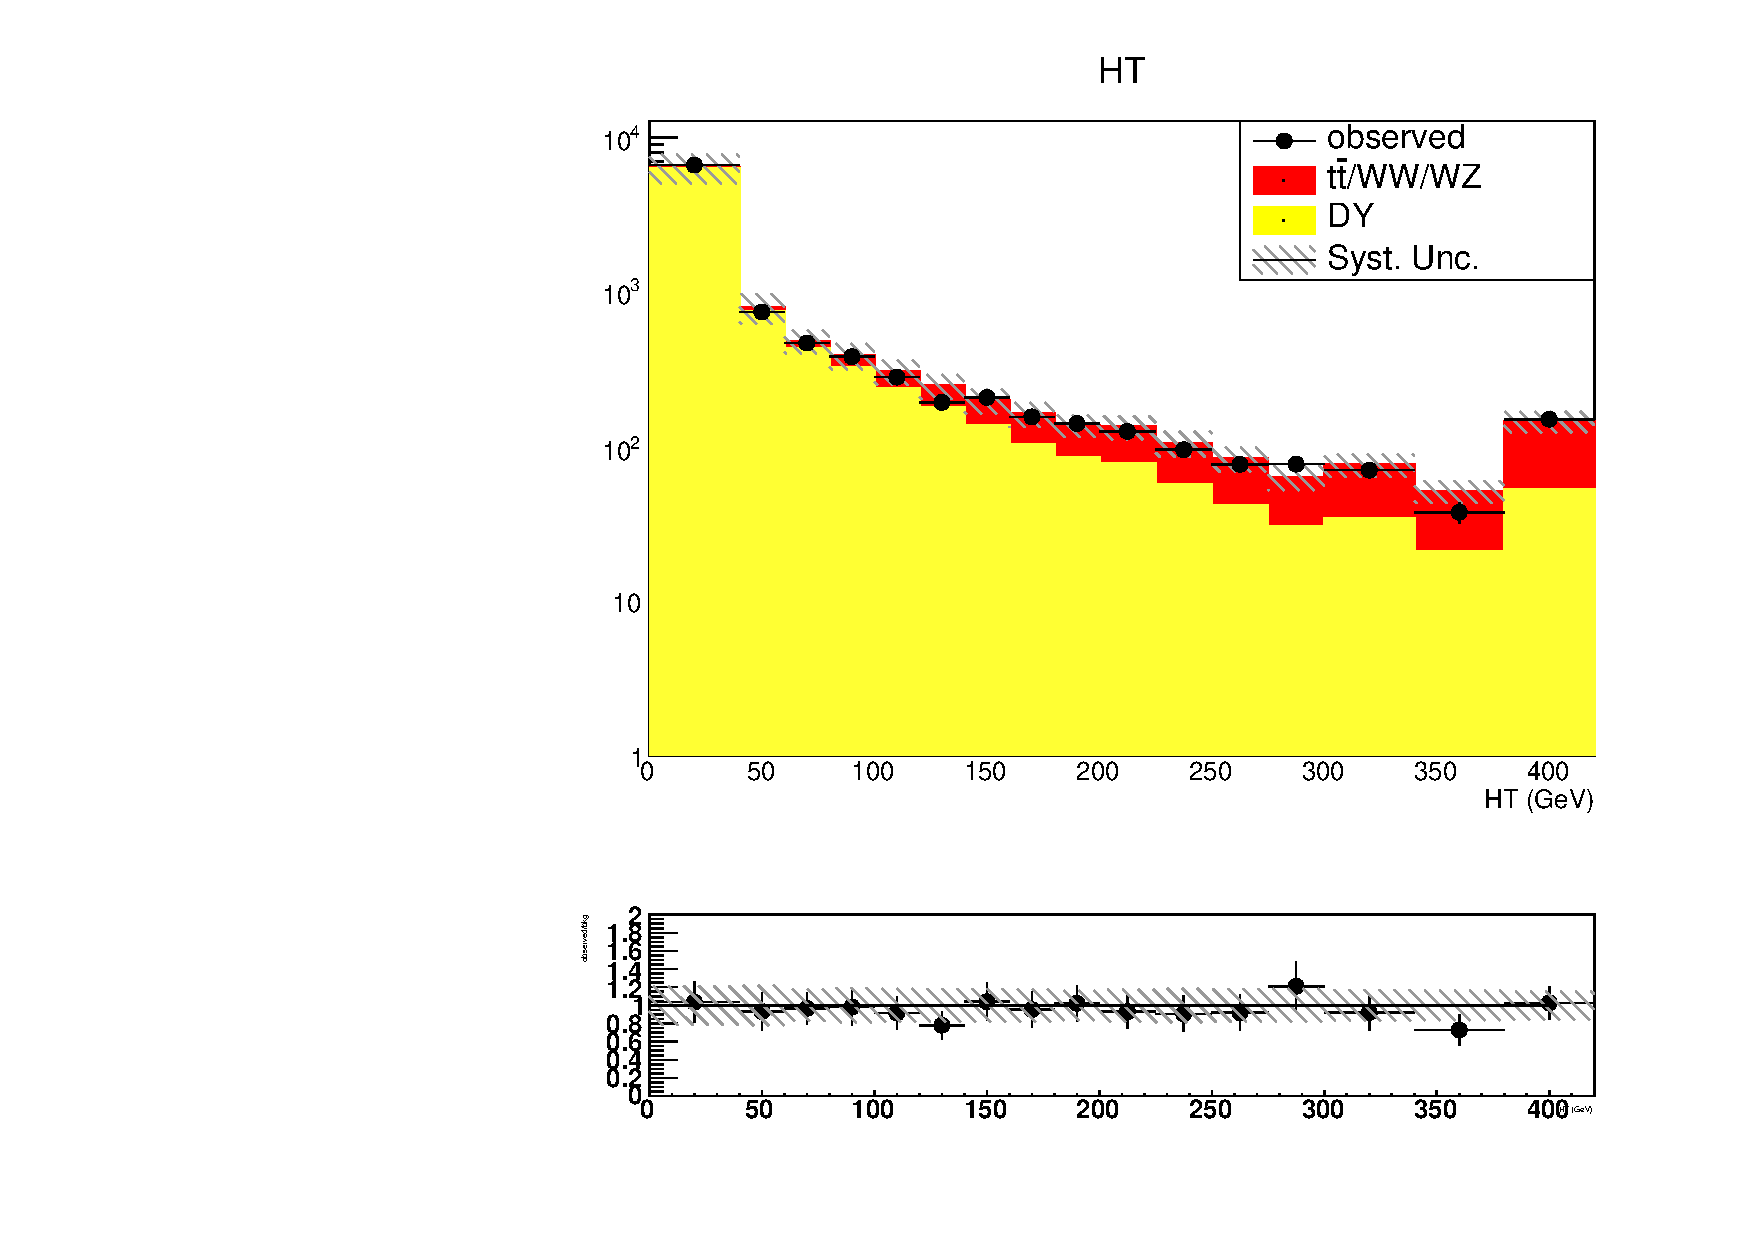
\includegraphics[width=0.45\textwidth]{Figures/closure_elefakepho_HT_egamma.pdf}
  \caption{Simulation closure test for electron misidentification estimation in the $e\gamma$ channel. The misidentification rate derived from Drell-Yan sample is applied to a combination of Drell-Yan, $t\bar{t}$ and WW samples. Top left: photon $p_T$; top right: $p_T^{miss}$; bottom left: $M_T$; bottom right: $HT$.}
  \label{fig:efakephoclosure_egamma}
\end{figure}


\begin{figure}
  \centering
    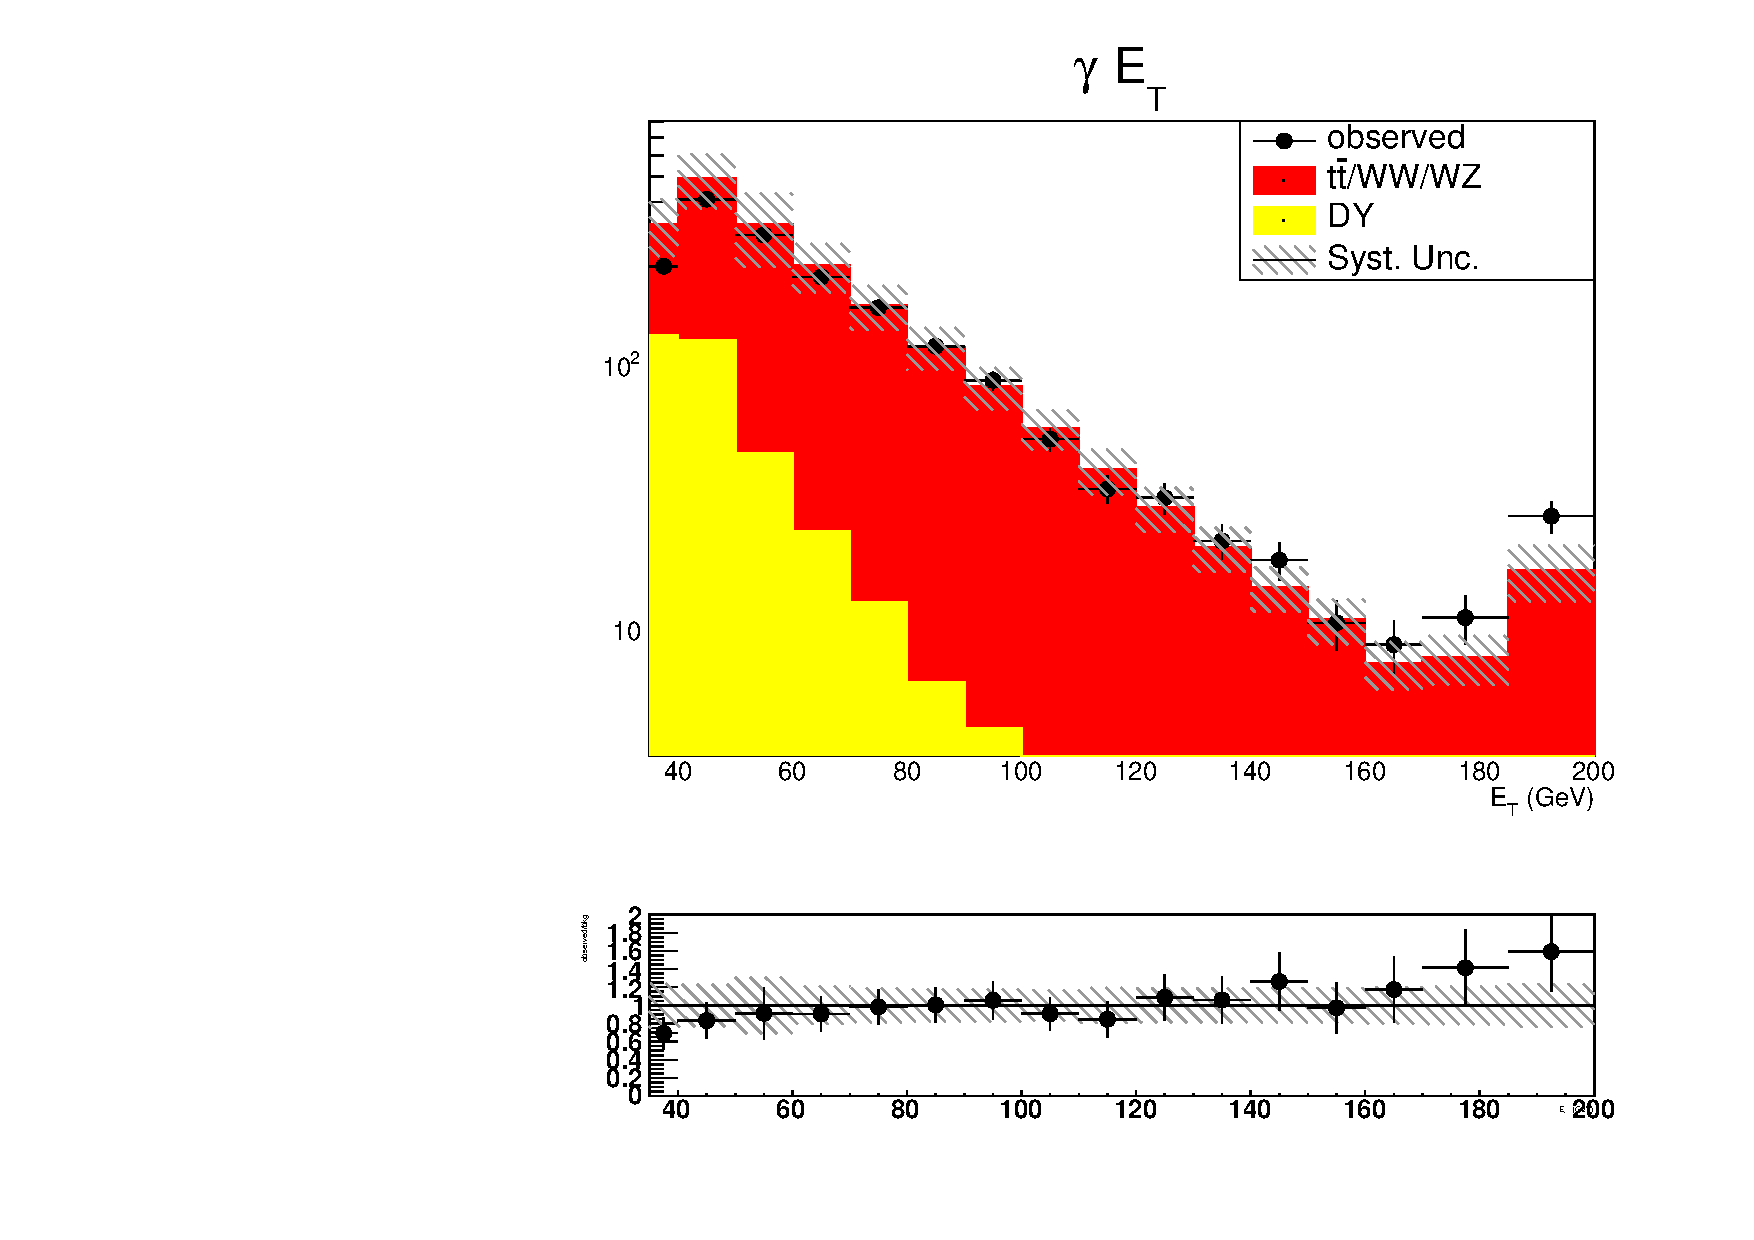
\includegraphics[width=0.45\textwidth]{Figures/closure_elefakepho_PhotonEt_mg.pdf}
    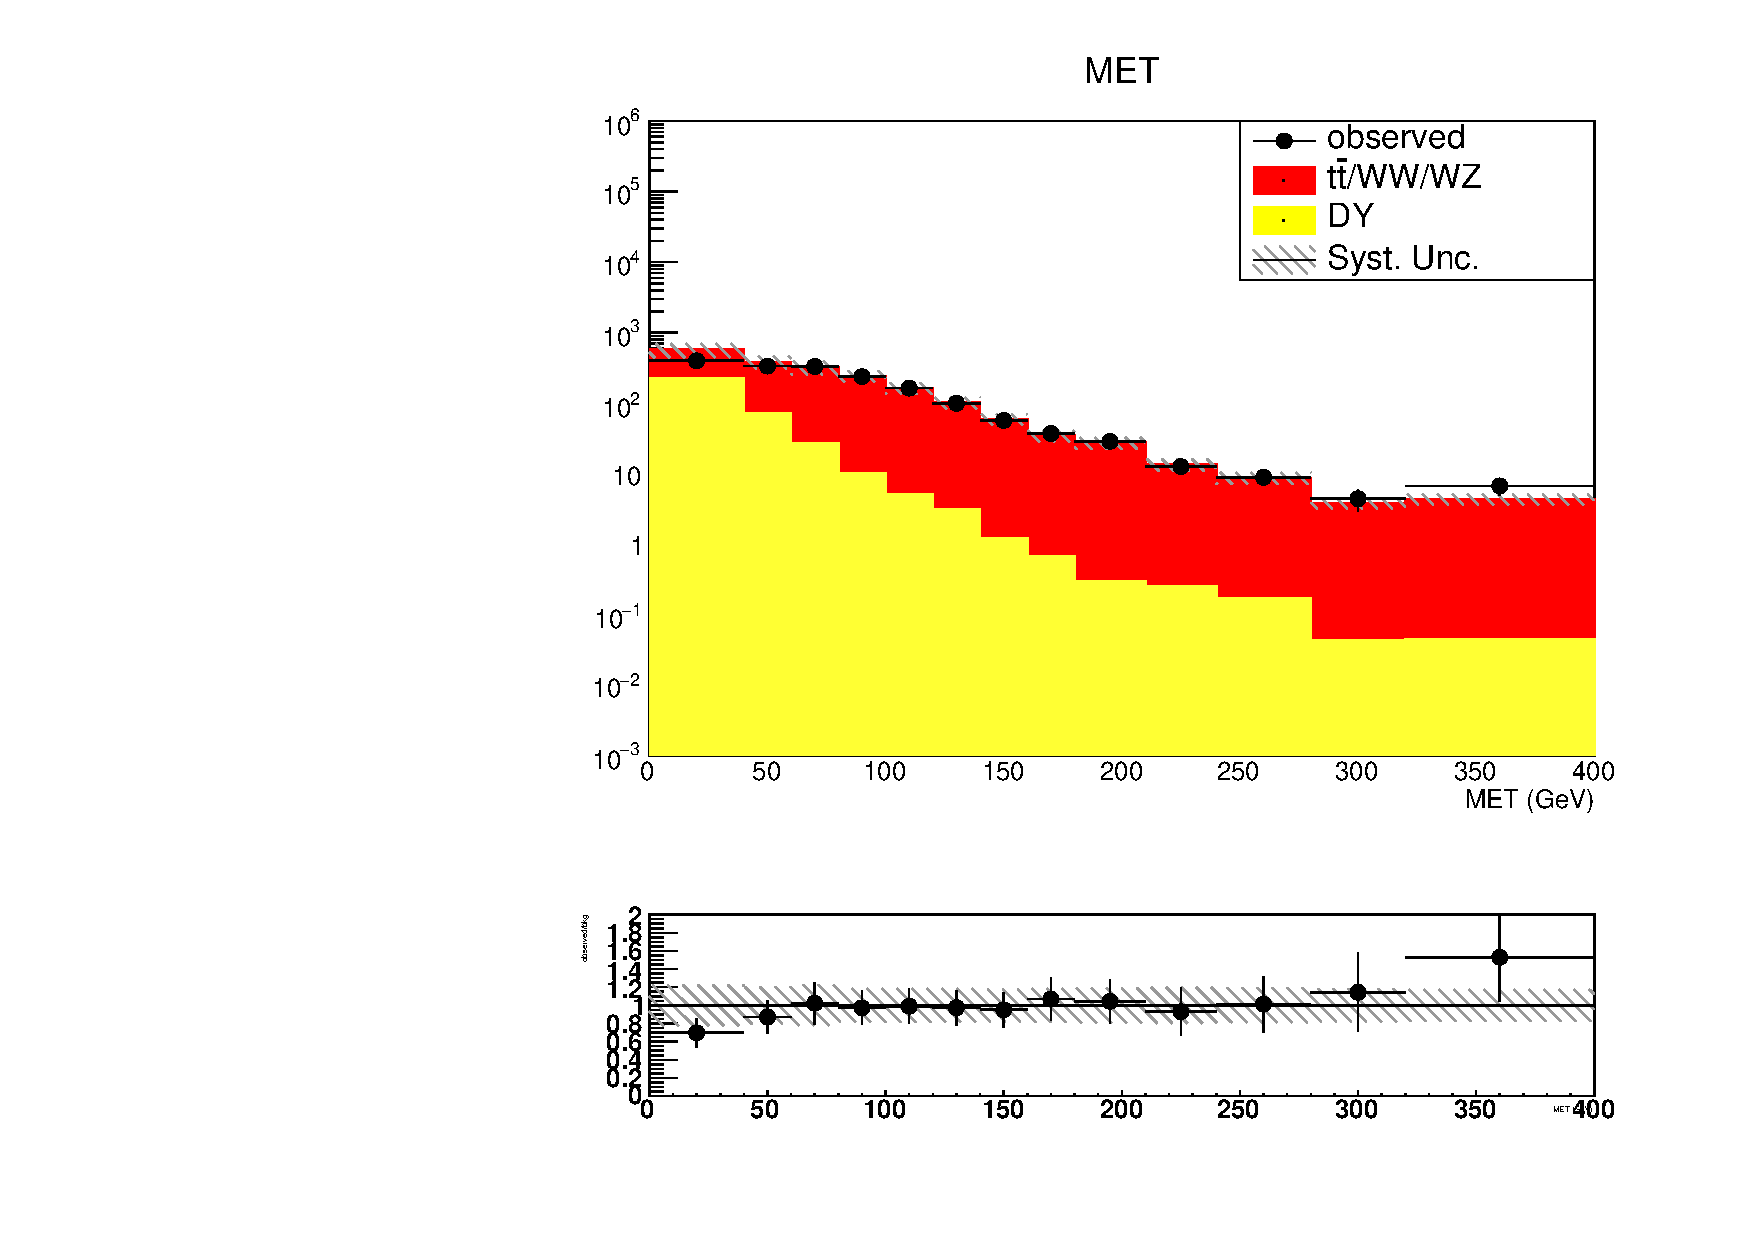
\includegraphics[width=0.45\textwidth]{Figures/closure_elefakepho_MET_mg.pdf}
    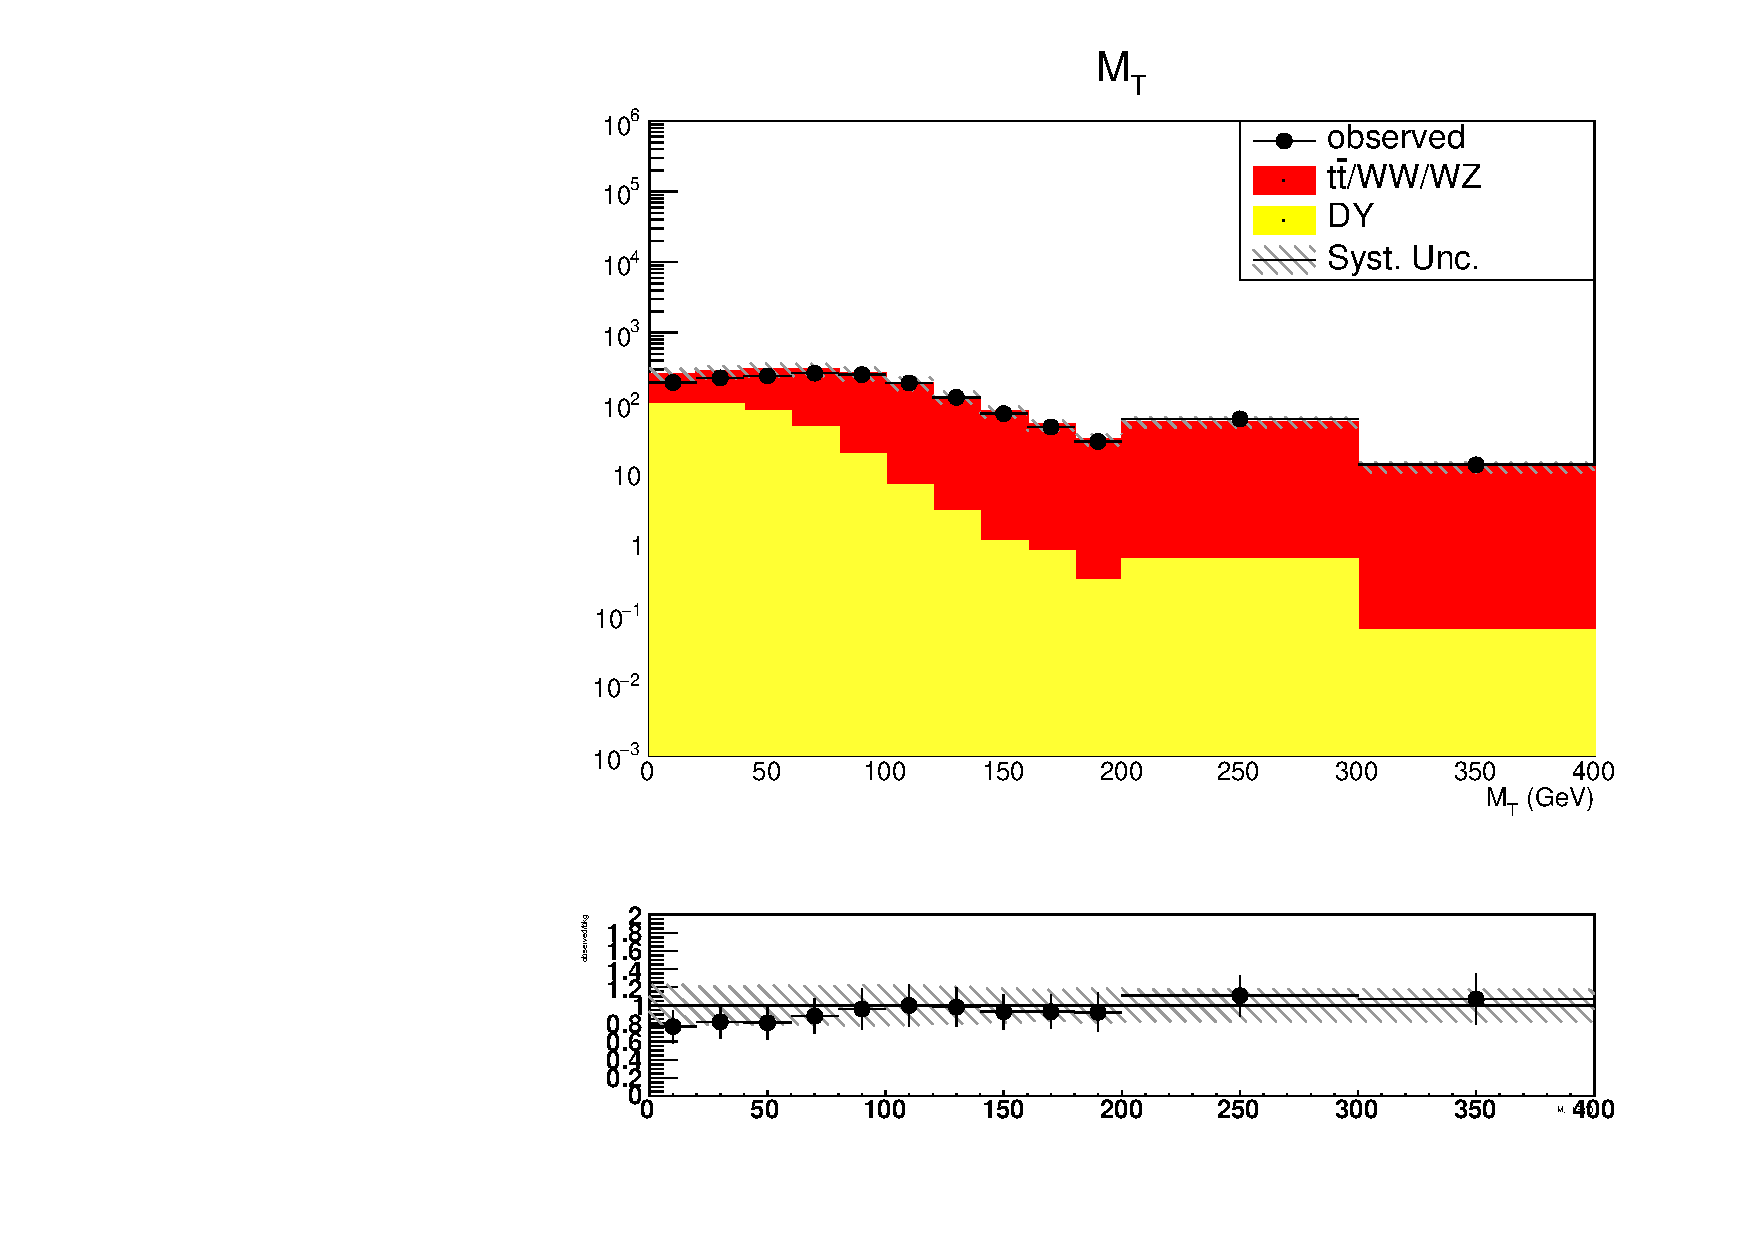
\includegraphics[width=0.45\textwidth]{Figures/closure_elefakepho_MT_mg.pdf}
    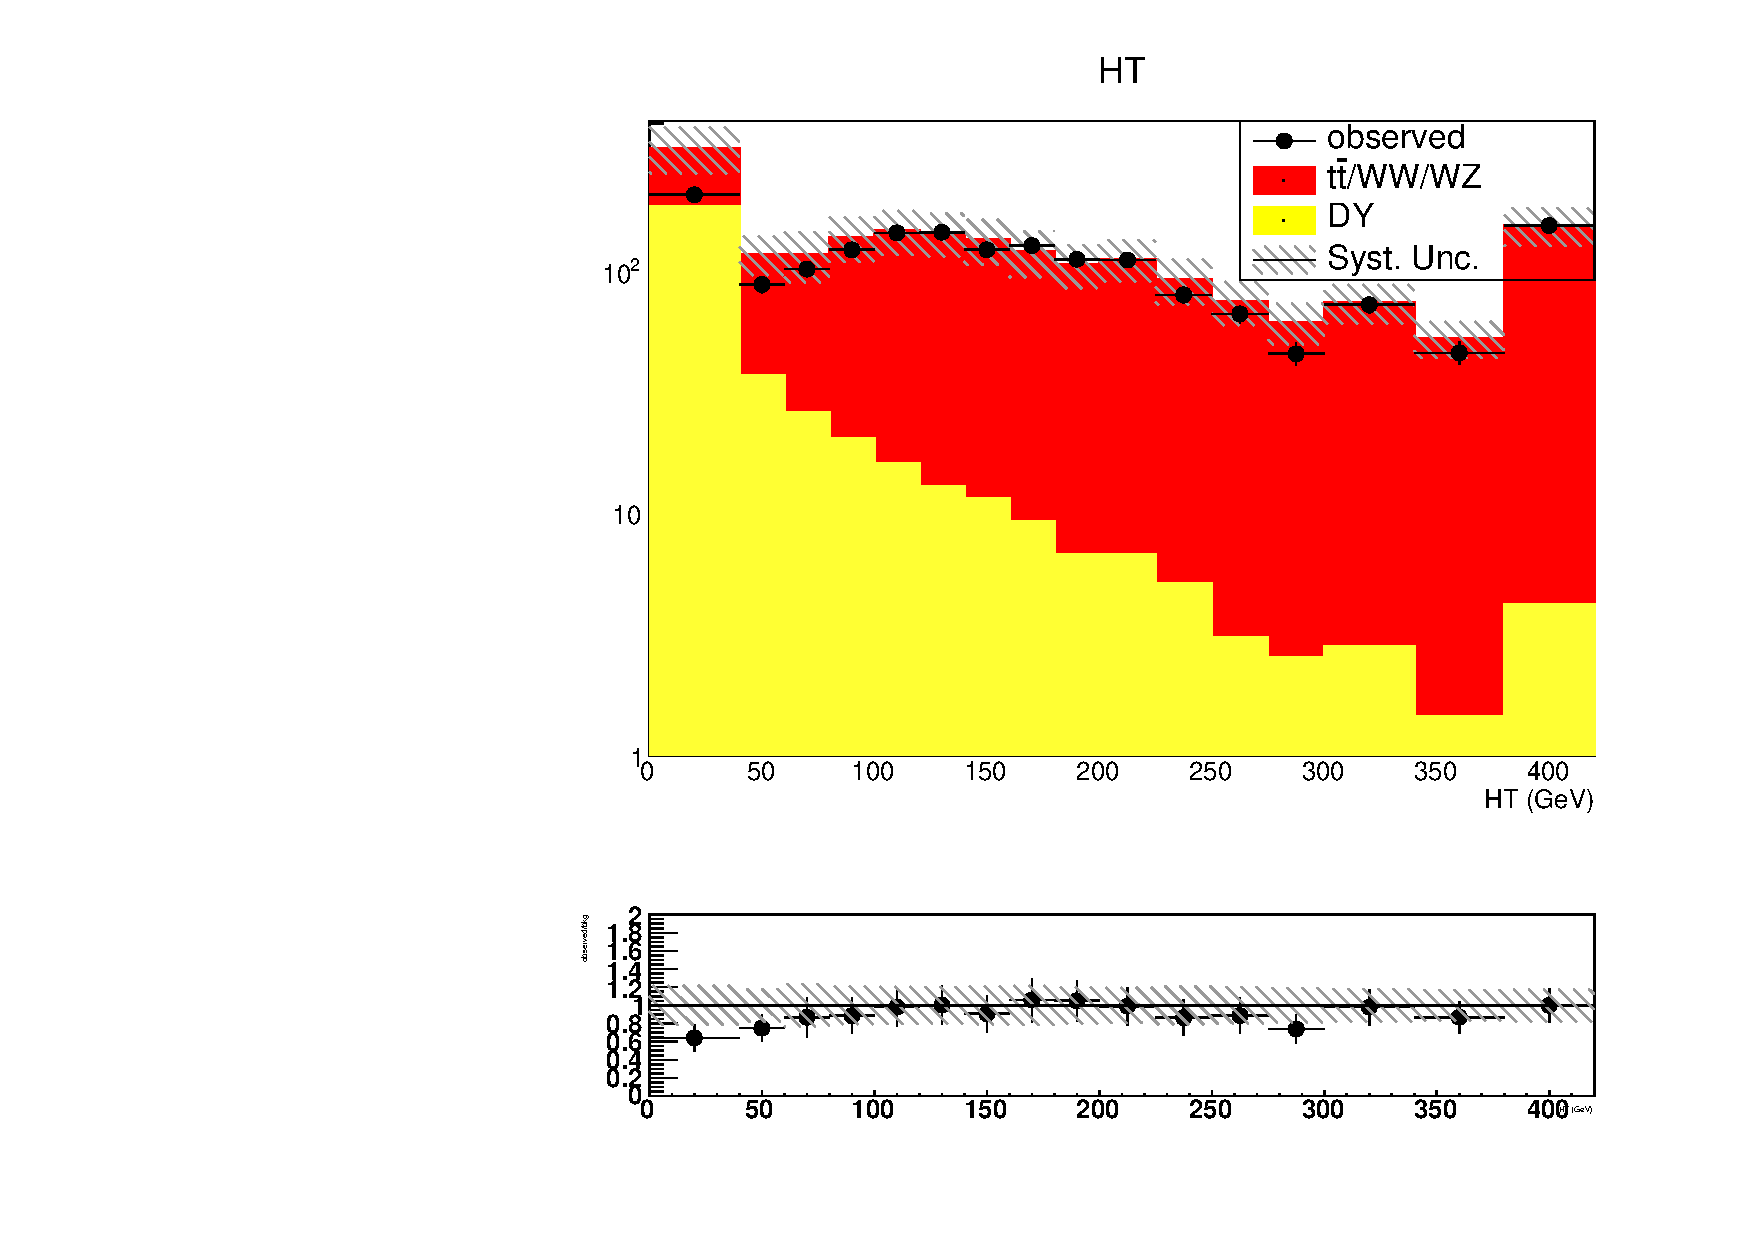
\includegraphics[width=0.45\textwidth]{Figures/closure_elefakepho_HT_mg.pdf}
  \caption{Simulation closure test for electron misidentification estimation in the $\mu\gamma$ channel. The misidentification rate derived from Drell-Yan sample is applied to a combination of Drell-Yan, $t\bar{t}$ and WW samples. Top left: photon $p_T$; top right: $p_T^{miss}$; bottom left: $M_T$; bottom right: $HT$.}
  \label{fig:efakephoclosure_mg}
\end{figure}


\section{The Misidentification of Hadrons as Photons}\label{subsec:jetfakepho}
Jets with electromagnetic fluctuations can deposit a significant fraction of energy in the ECAL and mimic photon signals. In particular, such misidentification occurs when the jet energy is mostly carried by a $\pi^0$ or $\eta$ which decays into two nearly collinear photons. \\

The jet to photon misidentification rate is low, but the cross section of QCD process is large, so the misidentified jets still have non-negligible contributions to the backgrounds. Such backgrounds are difficult to estimate using simulation because of the large statistics requirement and the possible mis-modeling of hadron fragmentation and hadronization. Therefore a data-driven method is deployed to predict this background. First, a proxy-to-fake transfer factor, defined as the ratio of estimated number of fake photons to the number of jet proxy objects, is derived in a low MET control region. This transfer factor will then be applied to a control sample with $e/\gamma$ enriched jets to predict the jet-to-photon fakes in the high MET signal region. \\

We compute the transfer factor in a $p_T^{miss} < $ 70 GeV control region. To calculate the ratio between the fake photons and jet proxies, we first need to determine the fraction of hadrons within the candidate photons.  Compared to the prompt photons, the fake photons tend to have wider shower shapes and more hadronic activities. Therefore we can use variables like $\sigma_{i\eta i\eta}$ and $Iso_{h^\pm}$ to discriminate between true photons and fakes. Figure \ref{fig:fakeinGJet} shows the $Iso_{h^\pm}$ contributions in the GJet simulation samples. \\

Because the fake and true components of the photon candidates have different $Iso_{h^\pm}$ shapes, we can determine the contribution of fake photons by a template fit to the isolation distribution of the photon objects. This fit is performed using the $p_T^{miss} <$ 70 GeV samples formed in the DoubleEG and MuonEG dataset for the $e\gamma$ and $\mu\gamma$ channel respectively. First, a well identified lepton passing all the offline selections including trigger matching is required. A photon is then selected with all identification criteria excluding the $\sigma_{i\eta i\eta}$ and $Iso_{h^\pm}$ cut. Trigger leg matching is also required for the photon in order to keep the same phase space as the signal photons. Out of such photons, those passing the shower shape cut, i.e. $\sigma_{i\eta i\eta} <$ 0.01031, are used as the fit target, and the $Iso_{h^\pm}$ distribution of the photons falling in the sideband 0.0103 $< \sigma_{i\eta i\eta} <$ 0.015 forms the hadronic template. The true photon template, on the other hand, is selected from the GJet simulation with the photon truth-matching to a generator level prompt photon. The fit to the $Iso_{h^\pm}$ distribution is performed using the ROOFIT package. \\

\begin{figure}
  \centering
    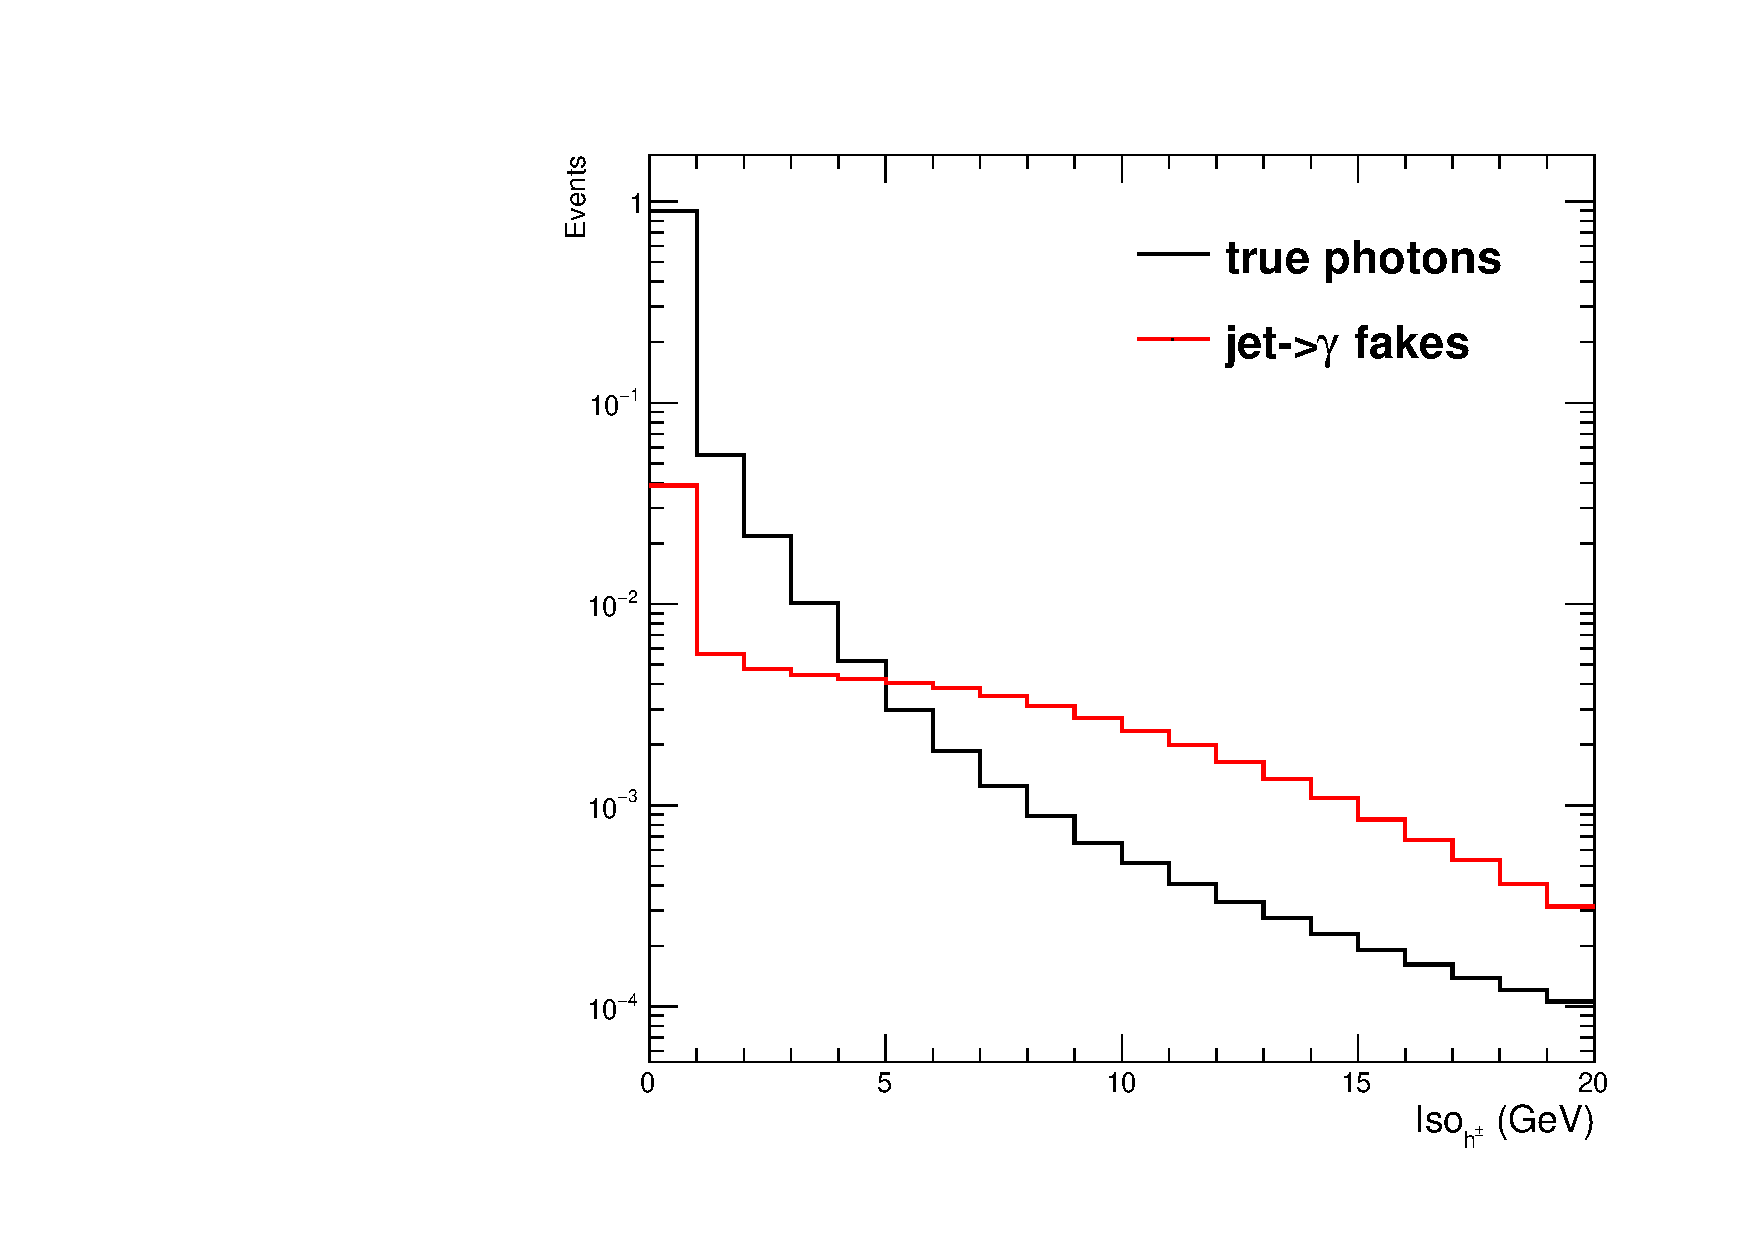
\includegraphics[width=0.5\textwidth]{Figures/PLOT_JetPhoTemplate.pdf}
  \caption{The normalized $Iso_{h^\pm}$ distributions of the true (black line) and fake (red line) photons in GJet sample.}
    \label{fig:fakeinGJet}
\end{figure}
\\

Once the normalization of the hadronic template is determined, an integral between 0 $< Iso_{h^\pm} <$ 1.295 is preformed on the template to estimate the number of fake photons in the candidate samples. The fraction of fake photons, $f$, is defined as: 
\begin{equation}
		f = \frac{N_{fake}}{N_{sig}}
\end{equation}
where $N_{fake}$ is the estimated number of fake photons passing $Iso_{h^\pm} < $ 1.295, and $N_{sig}$ is the number of events passing all the offline selections. \\

Though most of the true photons have narrow shower shape, a small fraction of the true photons still fall in the $\sigma_{i\eta i\eta}$ sideband and therefore contaminate the hadronic template. Having true photons in the hadronic template will result in overestimating the fraction of fakes. To correct the hadronic $Iso_{h^\pm}$ template shape, an iterative method is deployed to remove the true photon contaminations.\\

This method scales the normalized true photon $Iso_{h^\pm}$ shape taken from the GJet MC by a factor $N_{true-in-sb}$, and subtract this shape from the raw hadronic template. The factor, $N_{true-in-sb}$,  is calculated as:
\begin{equation}
		N_{true-in-sb} = N_{sig} \cdot (1-f_i) \cdot \frac{p_{sb}}{p_{sig}}
\end{equation}
where $f_i$ is the fraction of fakes estimated from the template fit in the $i$th iteration, $p_{sb}$ and $p_{sig}$ are the probability of a simulated true photon falling into the signal region and sideband region as illustrated in Figure \ref{fig:iteration}. This procedure is iteratively repeated several times until the calculated $f_i$ converges, i.e. $|f_i - f_{i+1}| < 0.001f_i$. This method is validated using the GJet simulation samples and shows a considerable improvement on the fake fraction estimation. The validation results are shown in Figure \ref{fig:GJetValidation} .

\begin{figure}
  \centering
    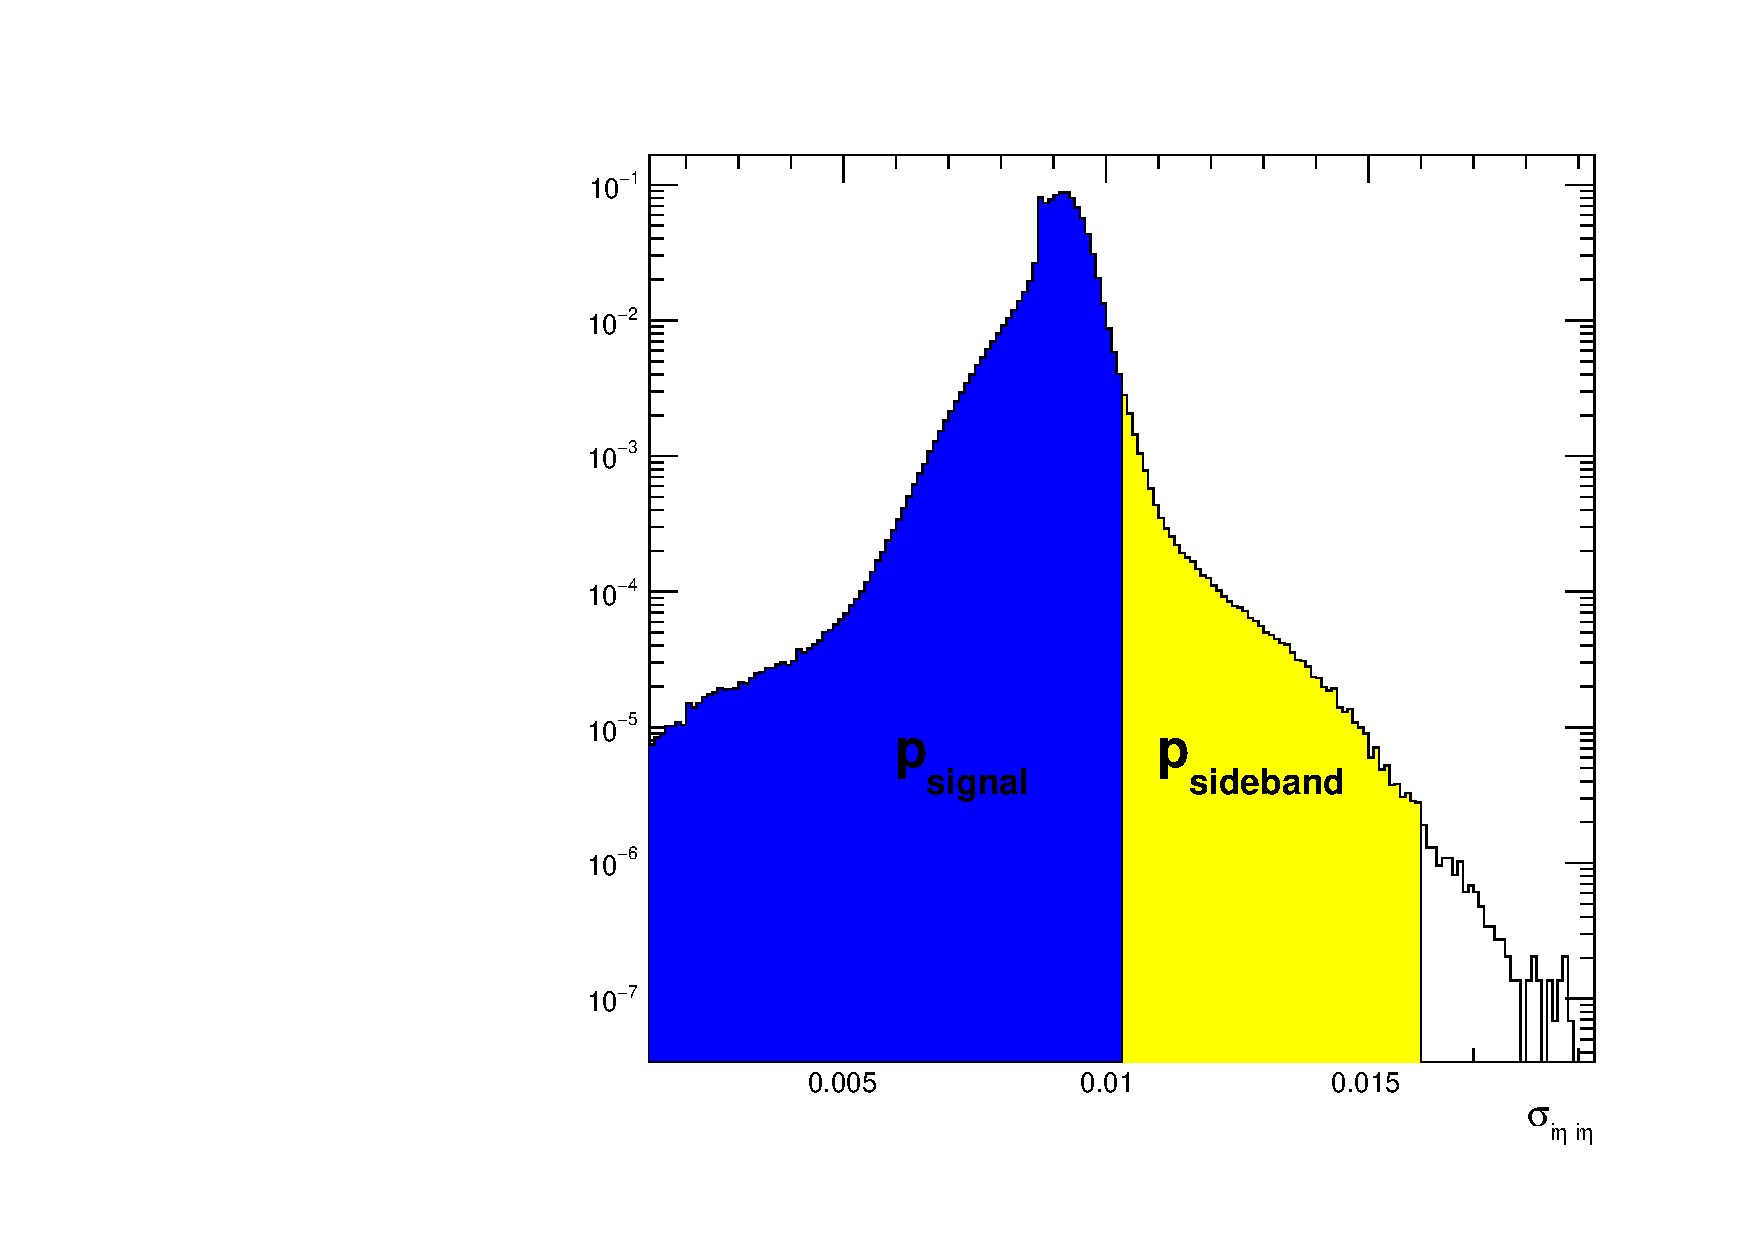
\includegraphics[width=0.5\textwidth]{Figures/PLOT_Iteration.pdf}
  \caption{The $\sigma_{i\eta i\eta}$ distribution of the true photons in GJet sample. Most of the true photons fall in signal region (blue), however, there is still a small fraction of true photons enter the sideband region (yellow).}
    \label{fig:iteration}
\end{figure}

\begin{figure}
  \centering
    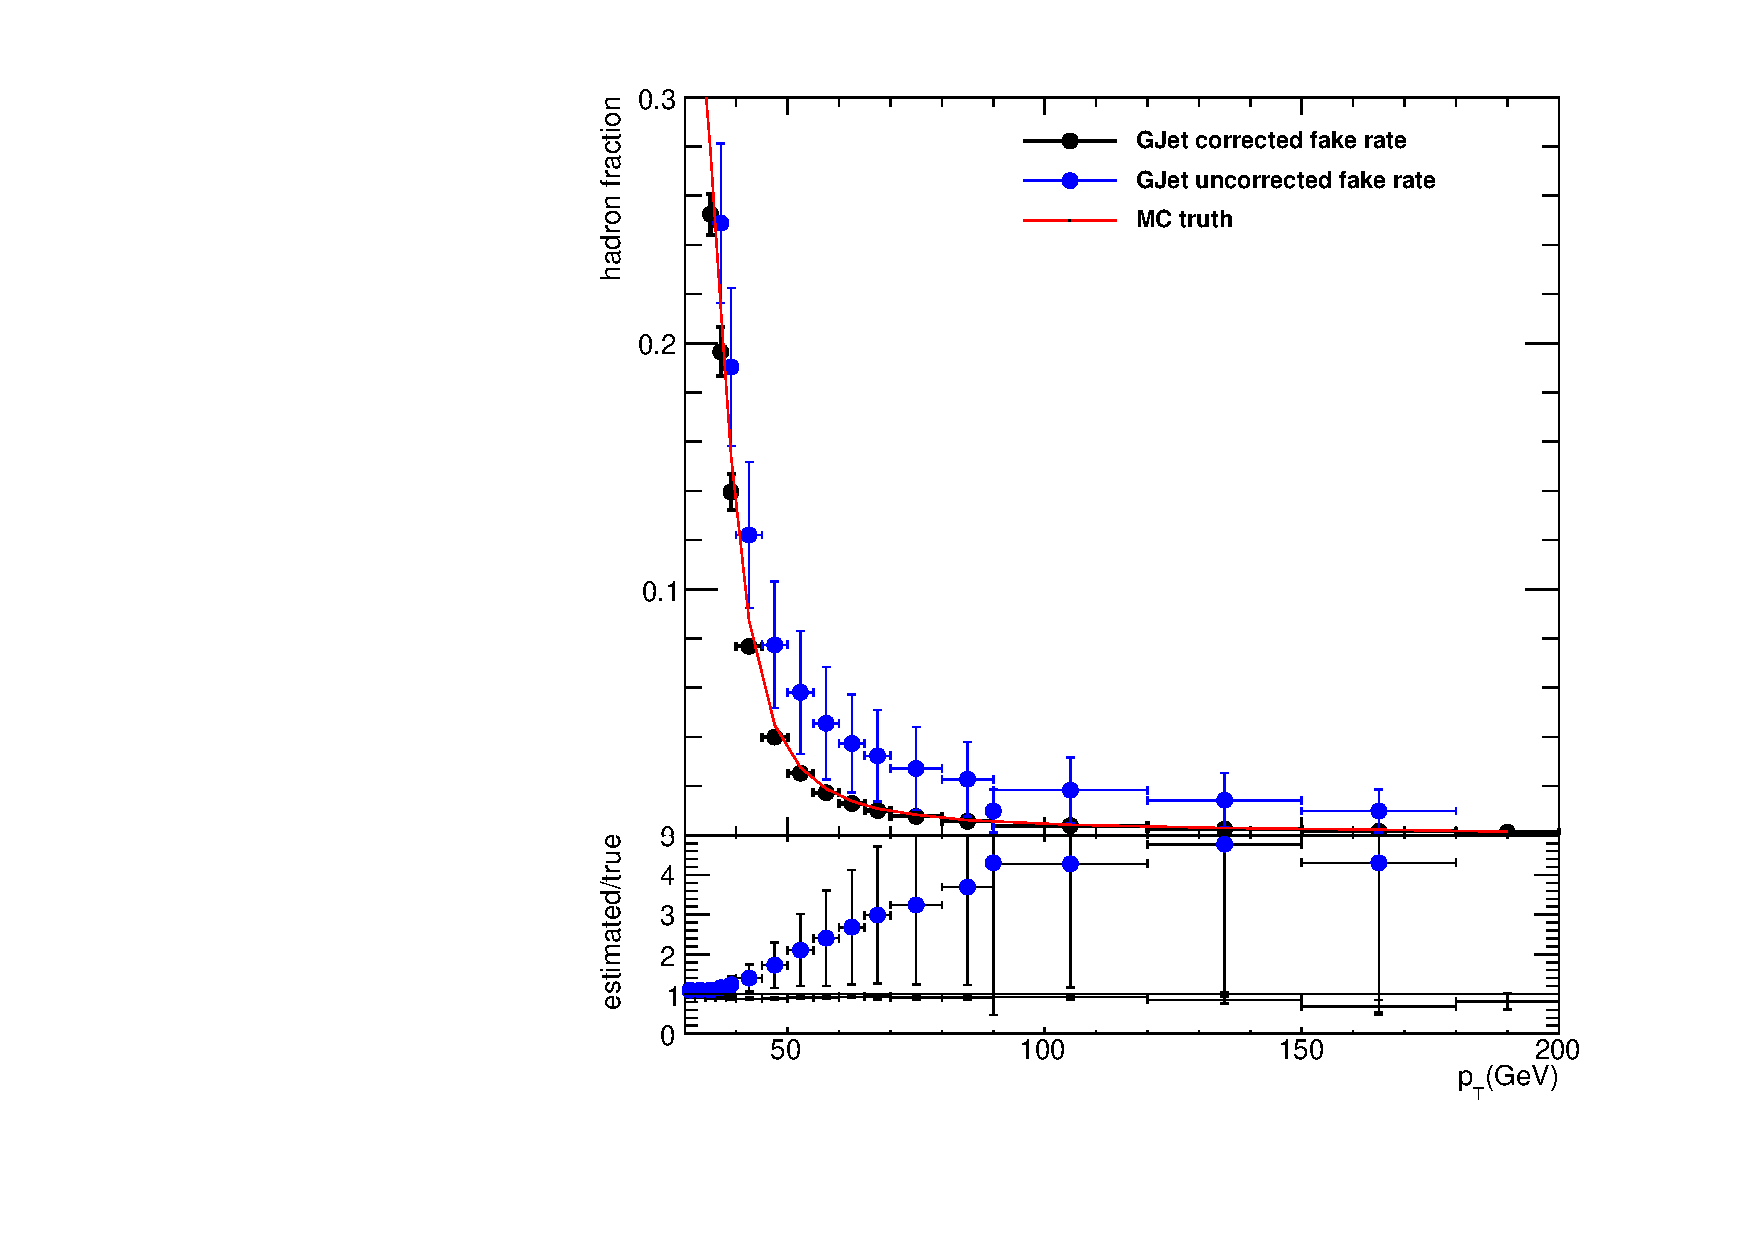
\includegraphics[width=0.5\textwidth]{Figures/JetFakePho_GJet.pdf}
  \caption{The hadron fractions estimated in GJet sample. The estimation with iteration corrections is shown in black dots, and the one without such correction is shown in blue.}
    \label{fig:GJetValidation}
\end{figure}

The $Iso_{h^\pm}$ fit is performed in 14 $p_T$ bins on the data. The fitting results for the $e\gamma$ channel is shown in Figure \ref{fig:DoubleEGjetfakebins}. The calculated fraction of fakes as a function of photon $p_T$ is shown in Figure \ref{fig:hadronfraction}. The fractions of hadrons are lower in the $\mu\gamma$ channel than those in the $e\gamma$ channel. This is because the MuonEG HLT trigger is seeded on isolated L1 objects, which have tighter isolation requirements than the $e\gamma$ trigger.

\begin{figure}
  \centering
    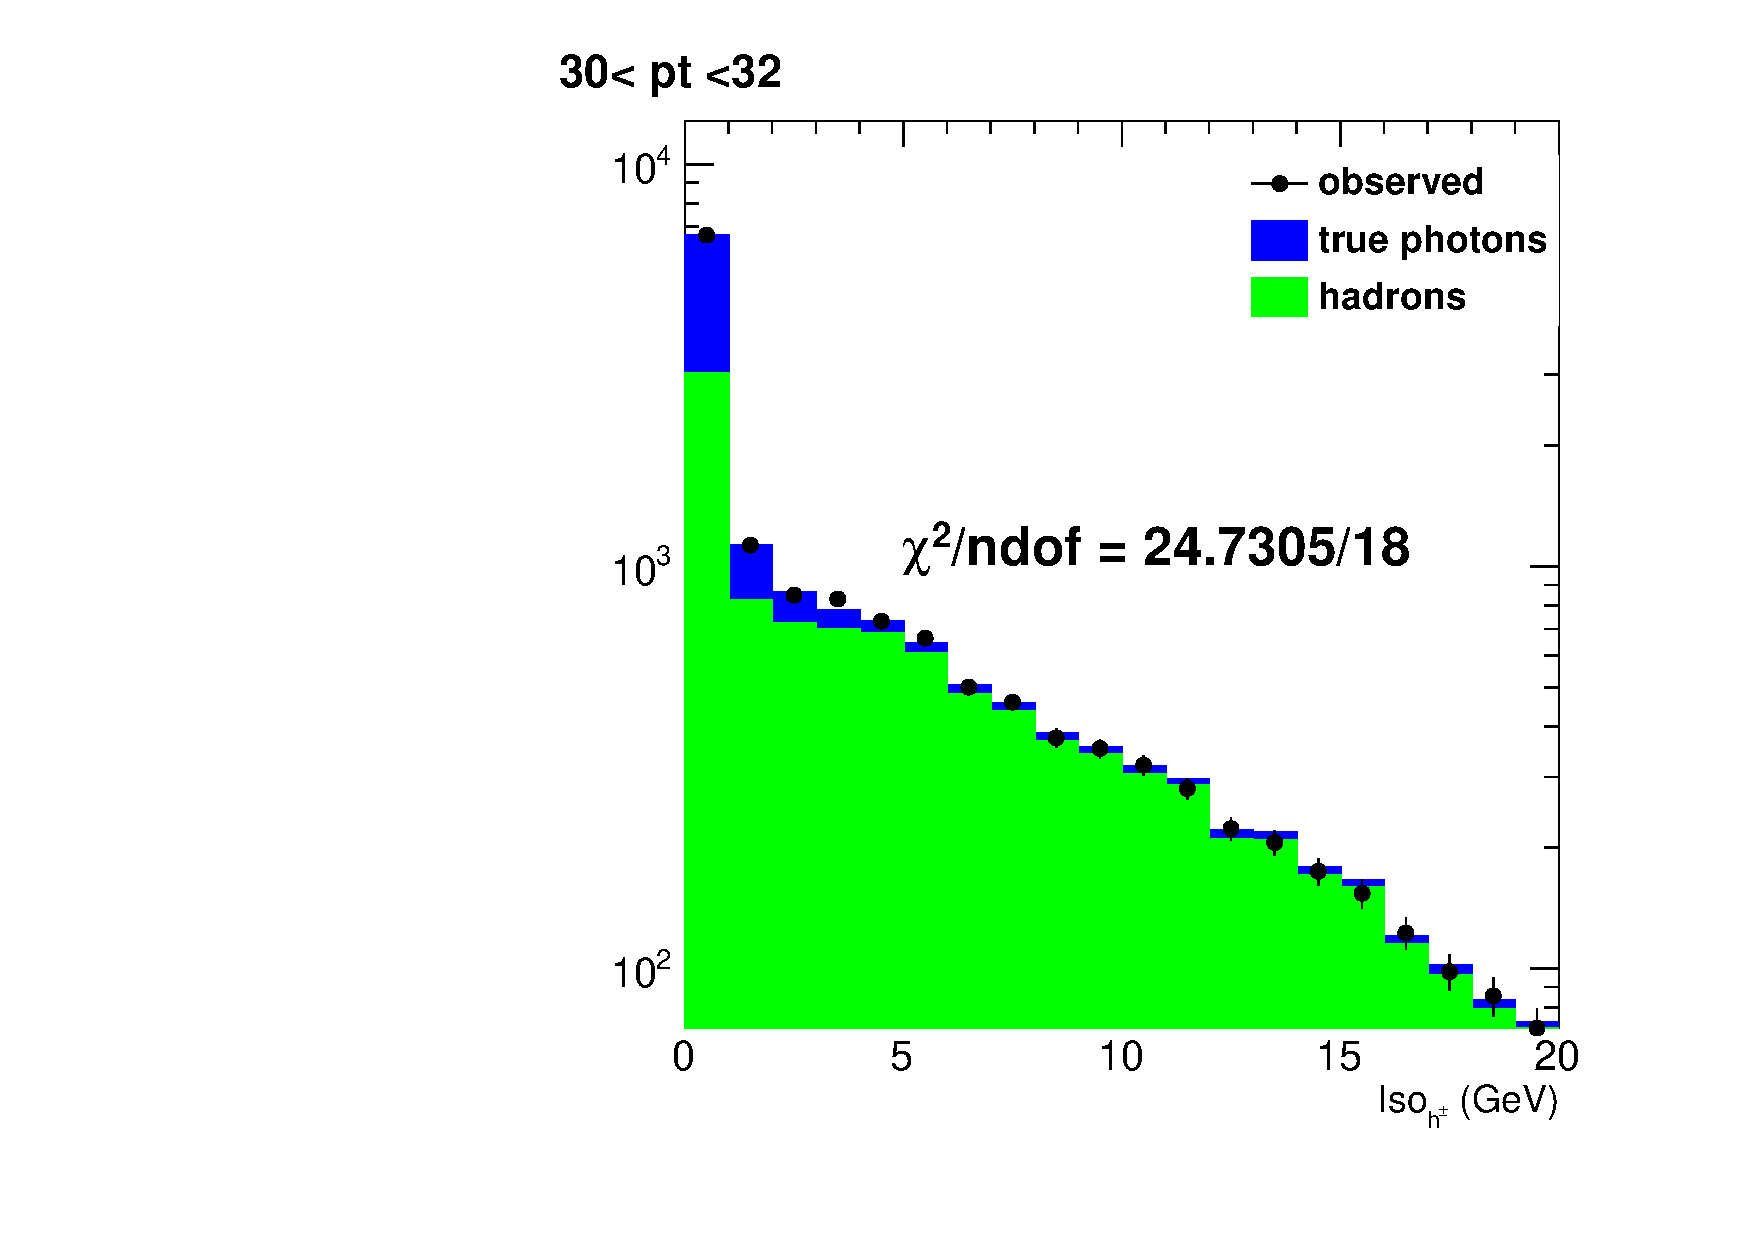
\includegraphics[width=0.32\textwidth]{Figures/frac-30-32_ChIso-DoubleEG-ReMiniAOD.pdf}   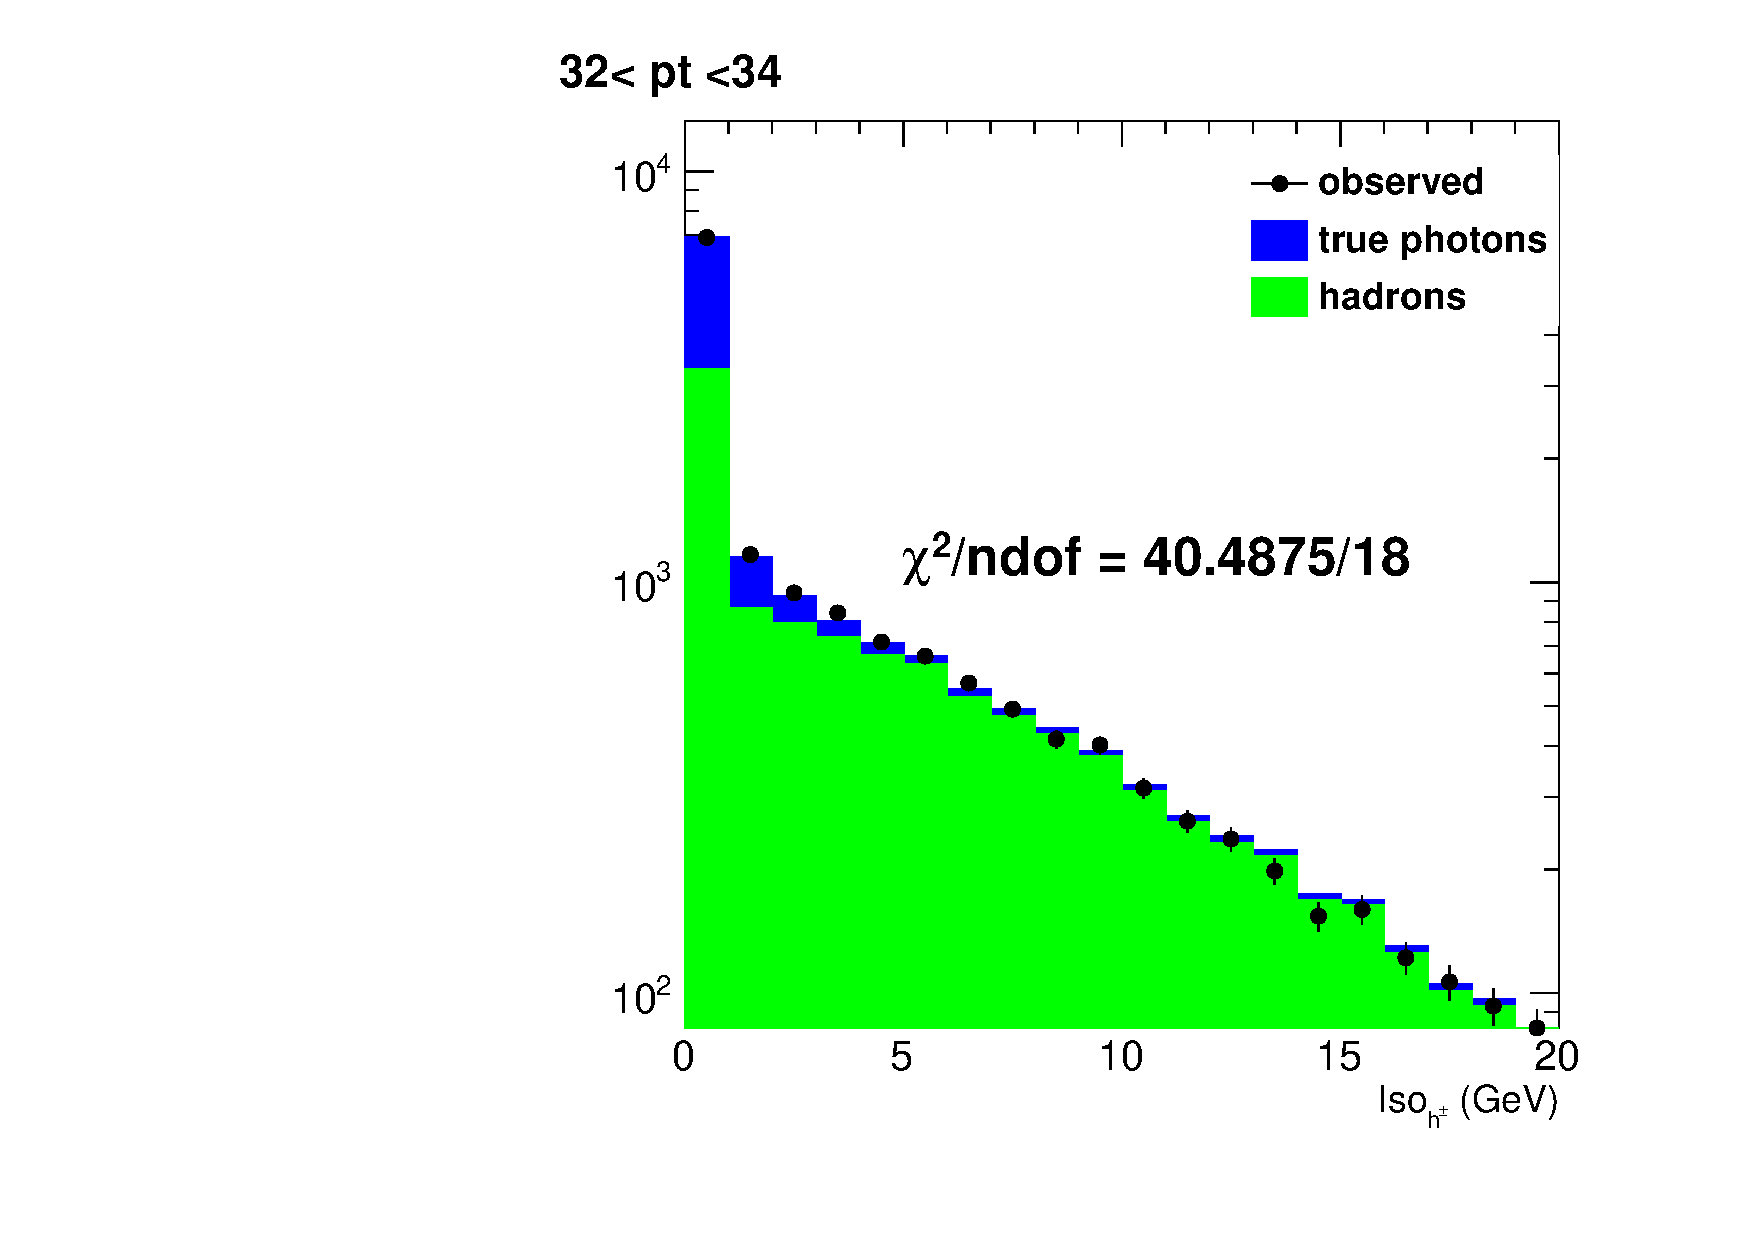
\includegraphics[width=0.32\textwidth]{Figures/frac-32-34_ChIso-DoubleEG-ReMiniAOD.pdf}         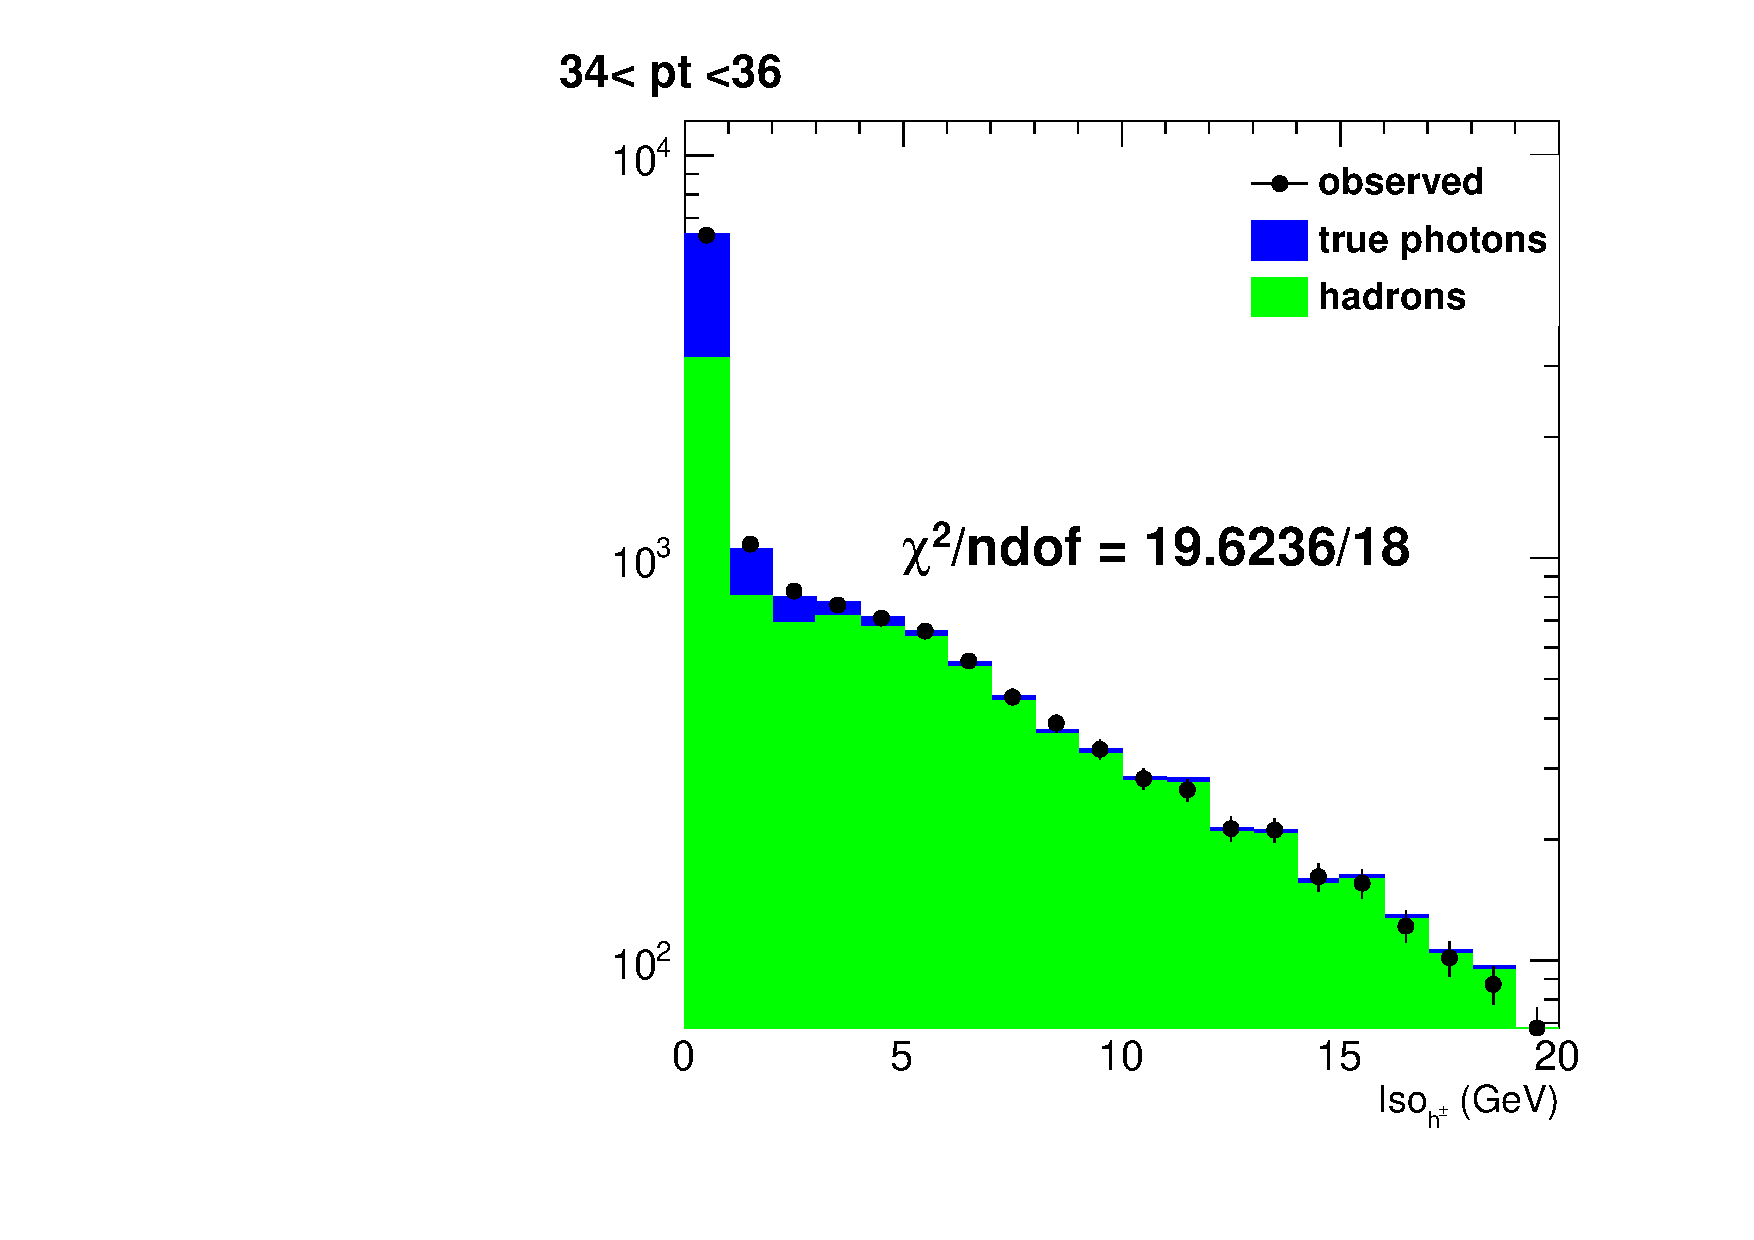
\includegraphics[width=0.32\textwidth]{Figures/frac-34-36_ChIso-DoubleEG-ReMiniAOD.pdf} \\
       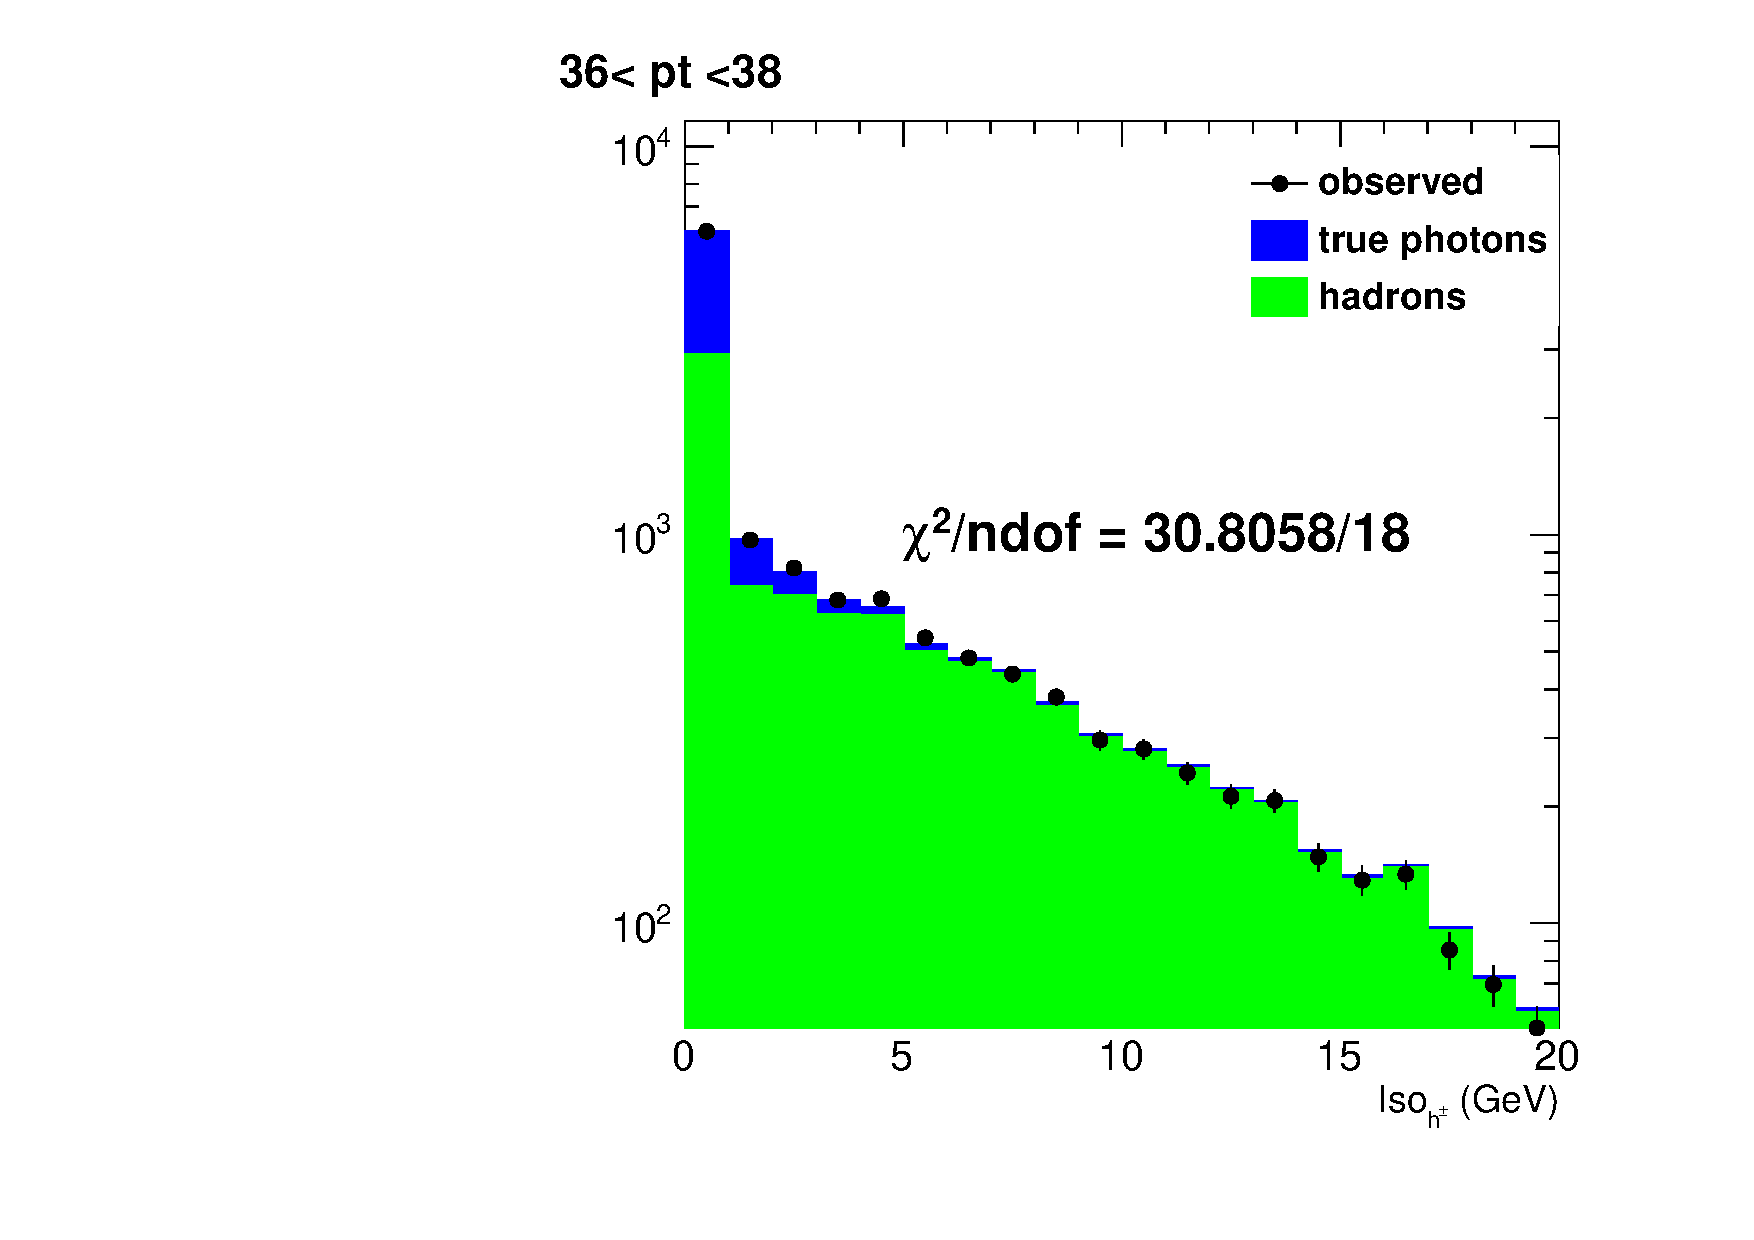
\includegraphics[width=0.32\textwidth]{Figures/frac-36-38_ChIso-DoubleEG-ReMiniAOD.pdf}   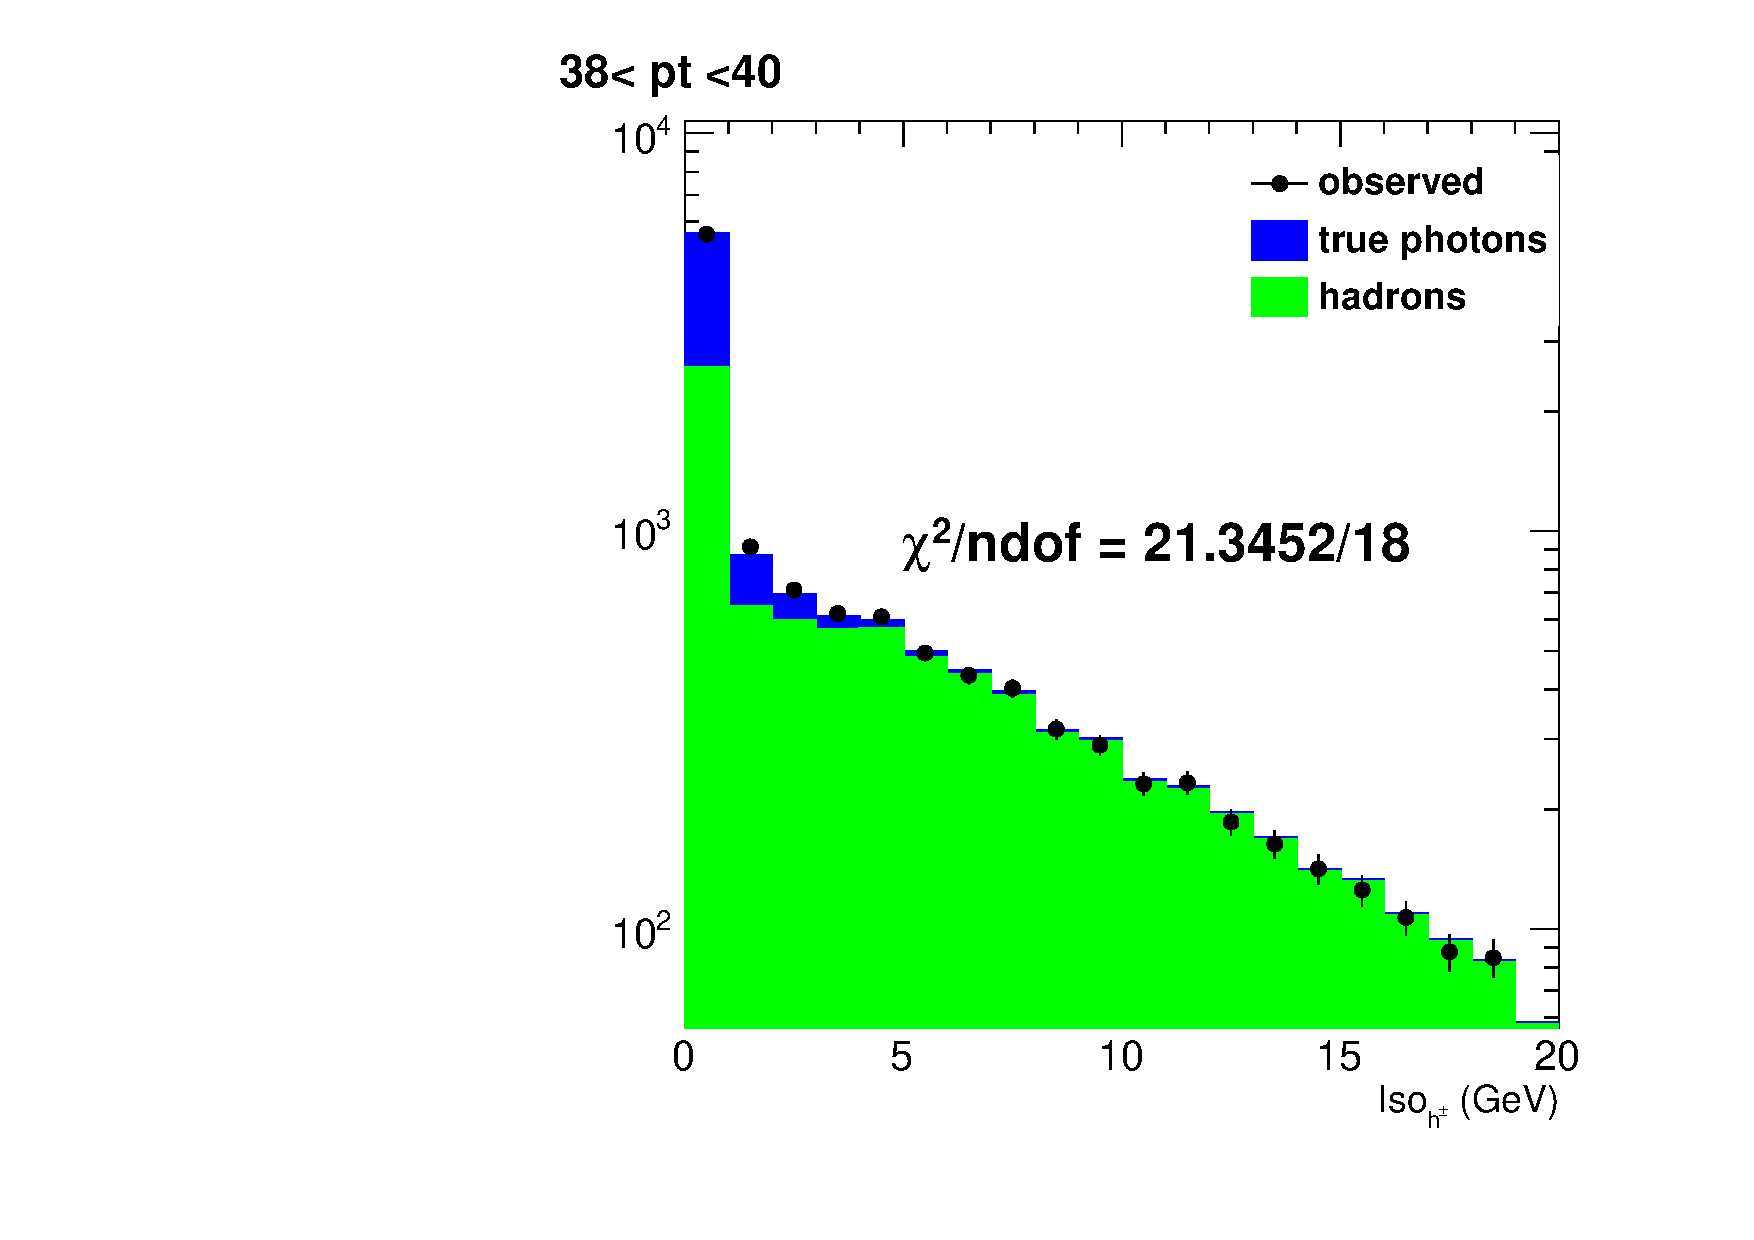
\includegraphics[width=0.32\textwidth]{Figures/frac-38-40_ChIso-DoubleEG-ReMiniAOD.pdf}         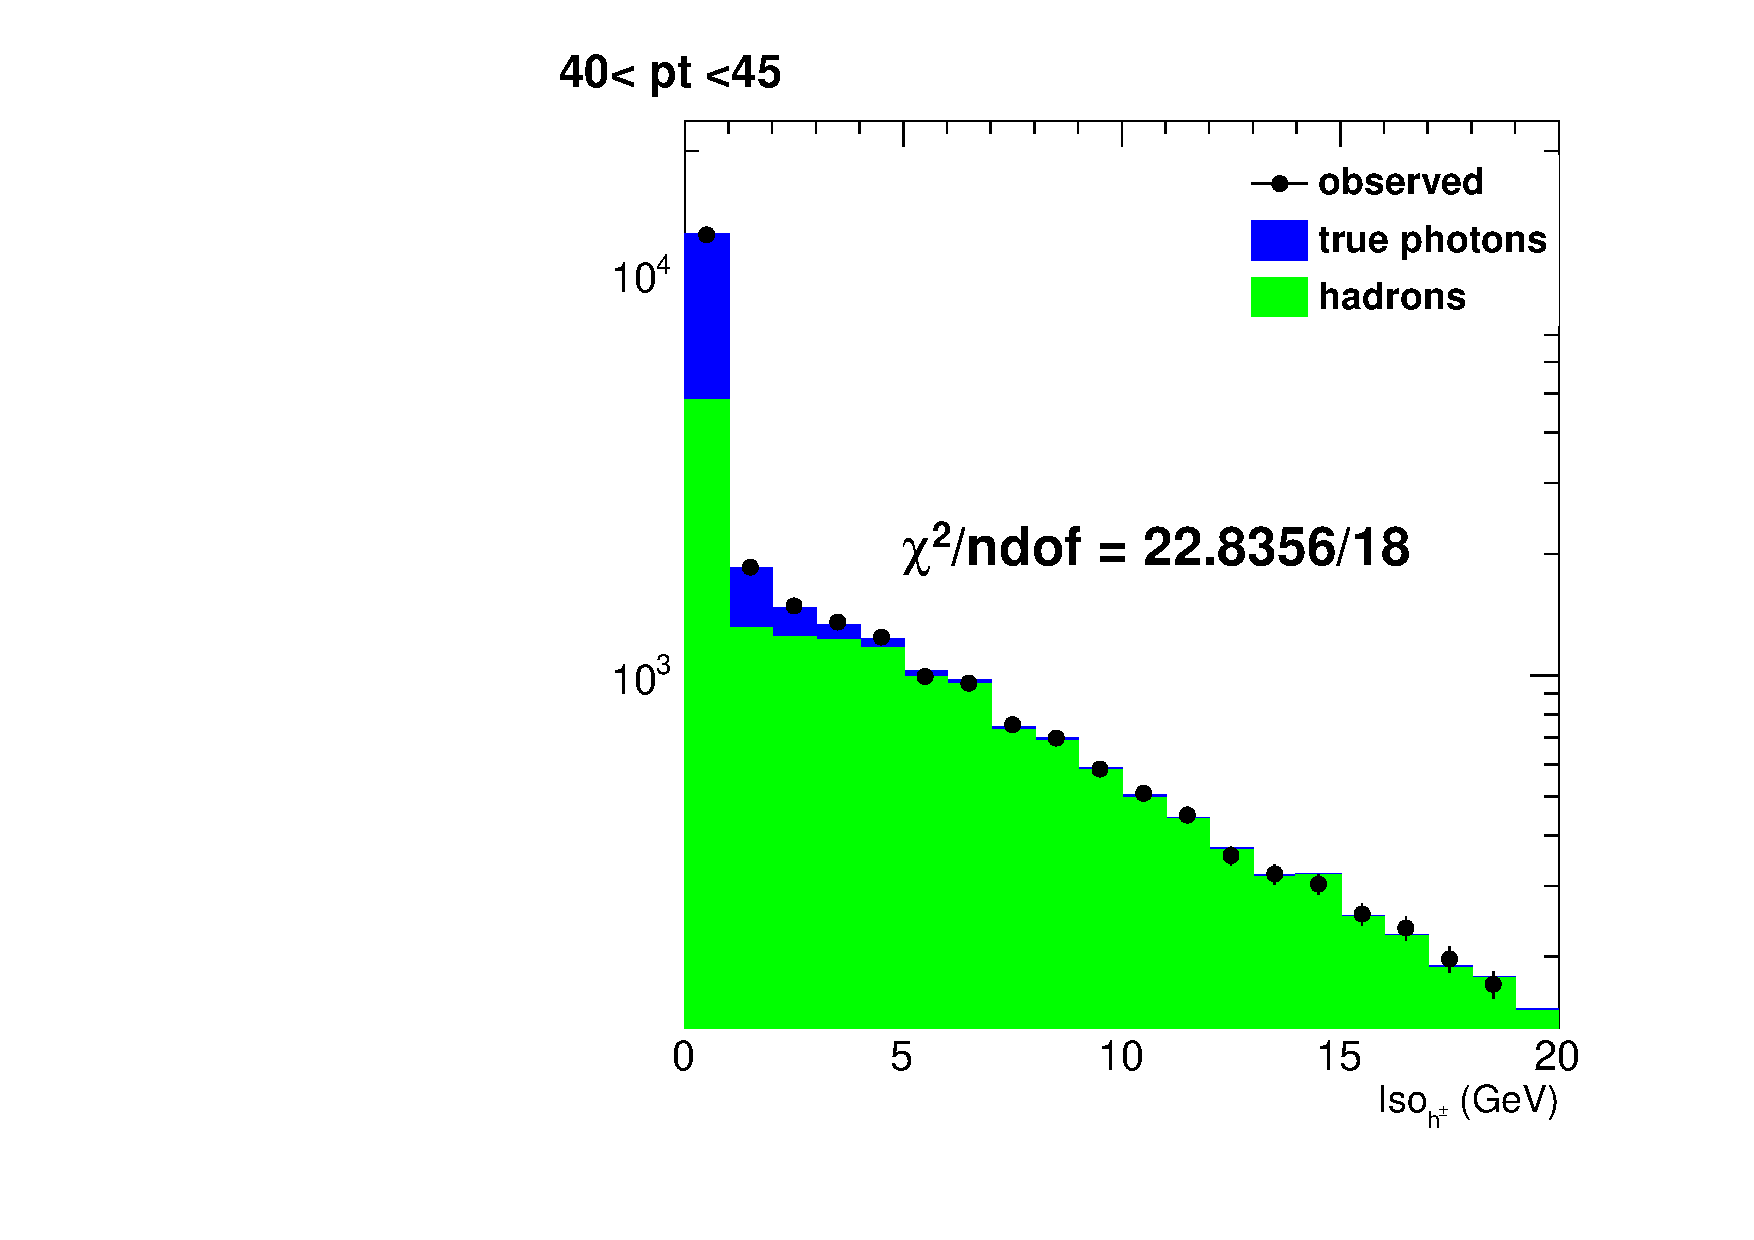
\includegraphics[width=0.32\textwidth]{Figures/frac-40-45_ChIso-DoubleEG-ReMiniAOD.pdf} \\
   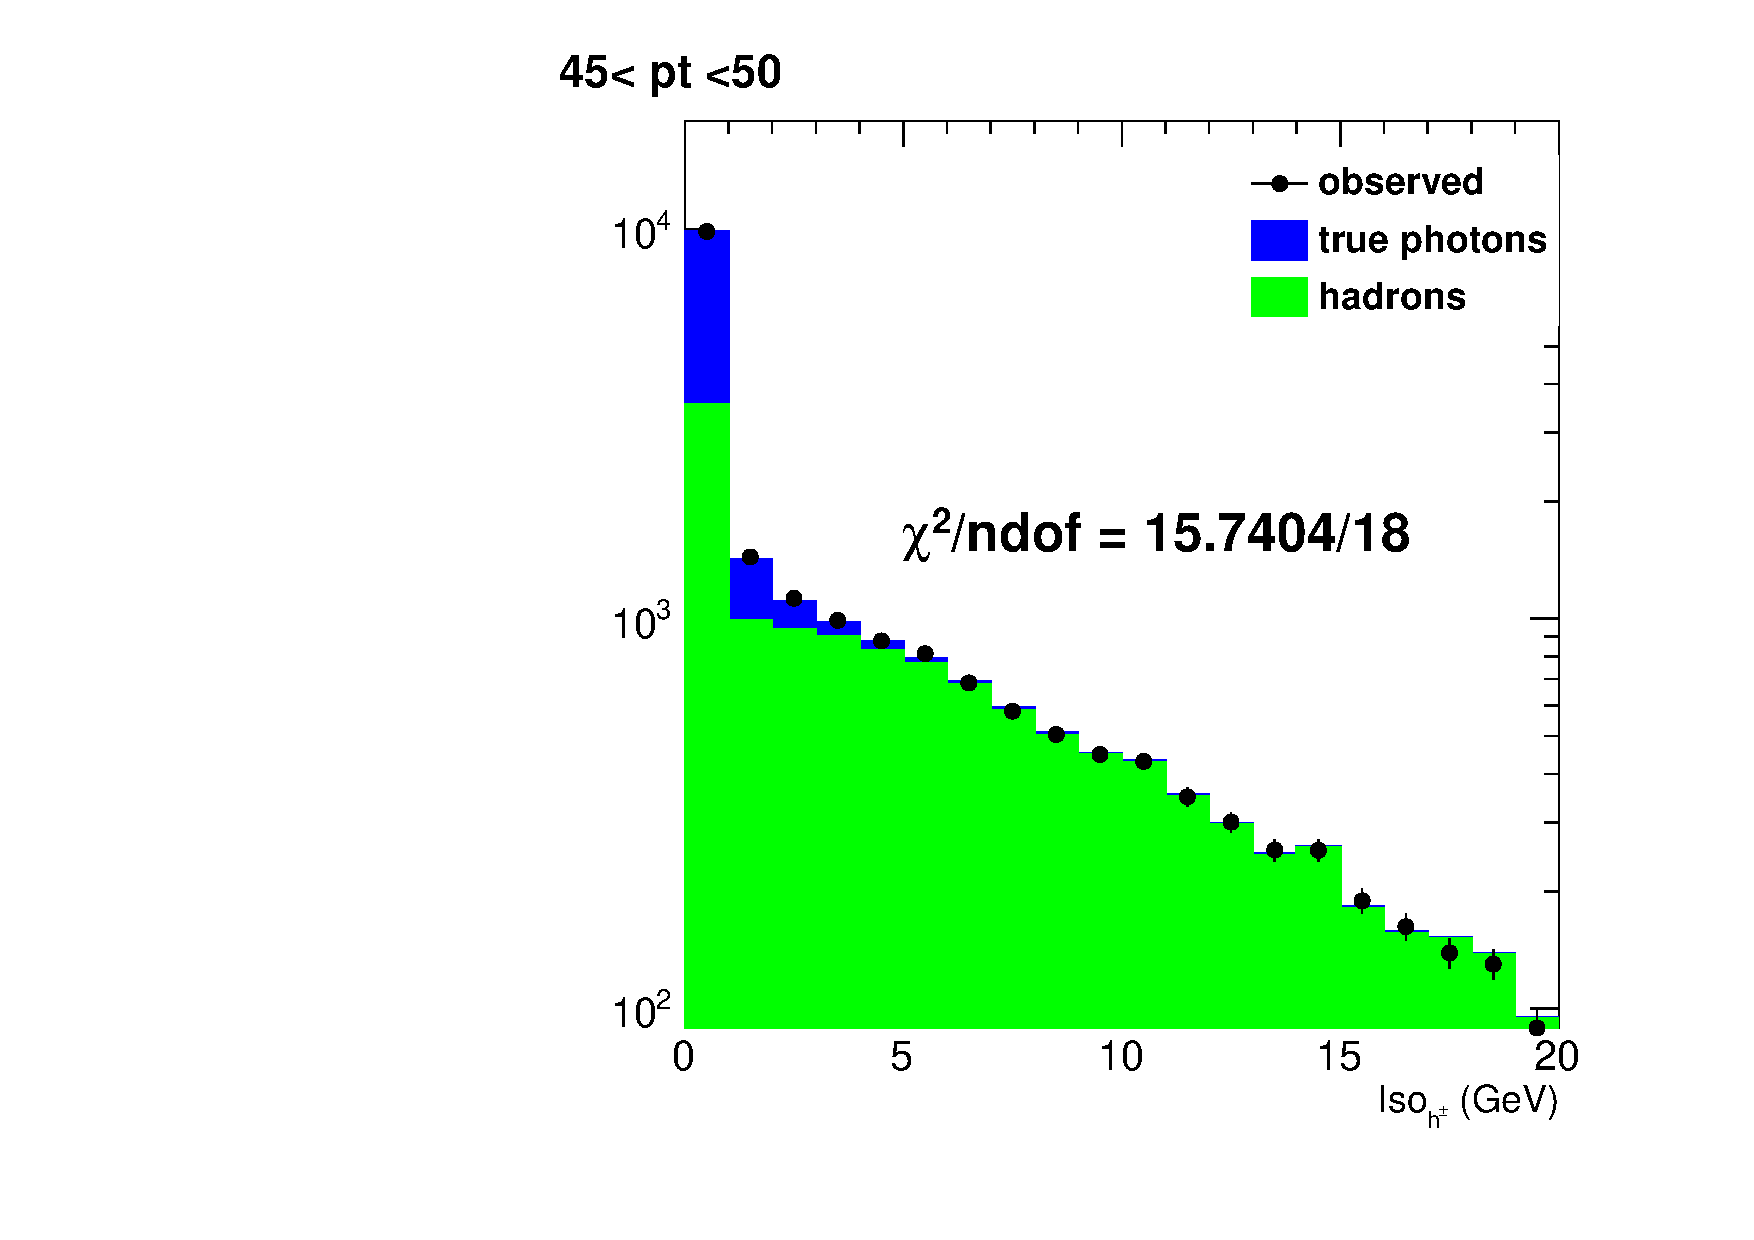
\includegraphics[width=0.32\textwidth]{Figures/frac-45-50_ChIso-DoubleEG-ReMiniAOD.pdf}   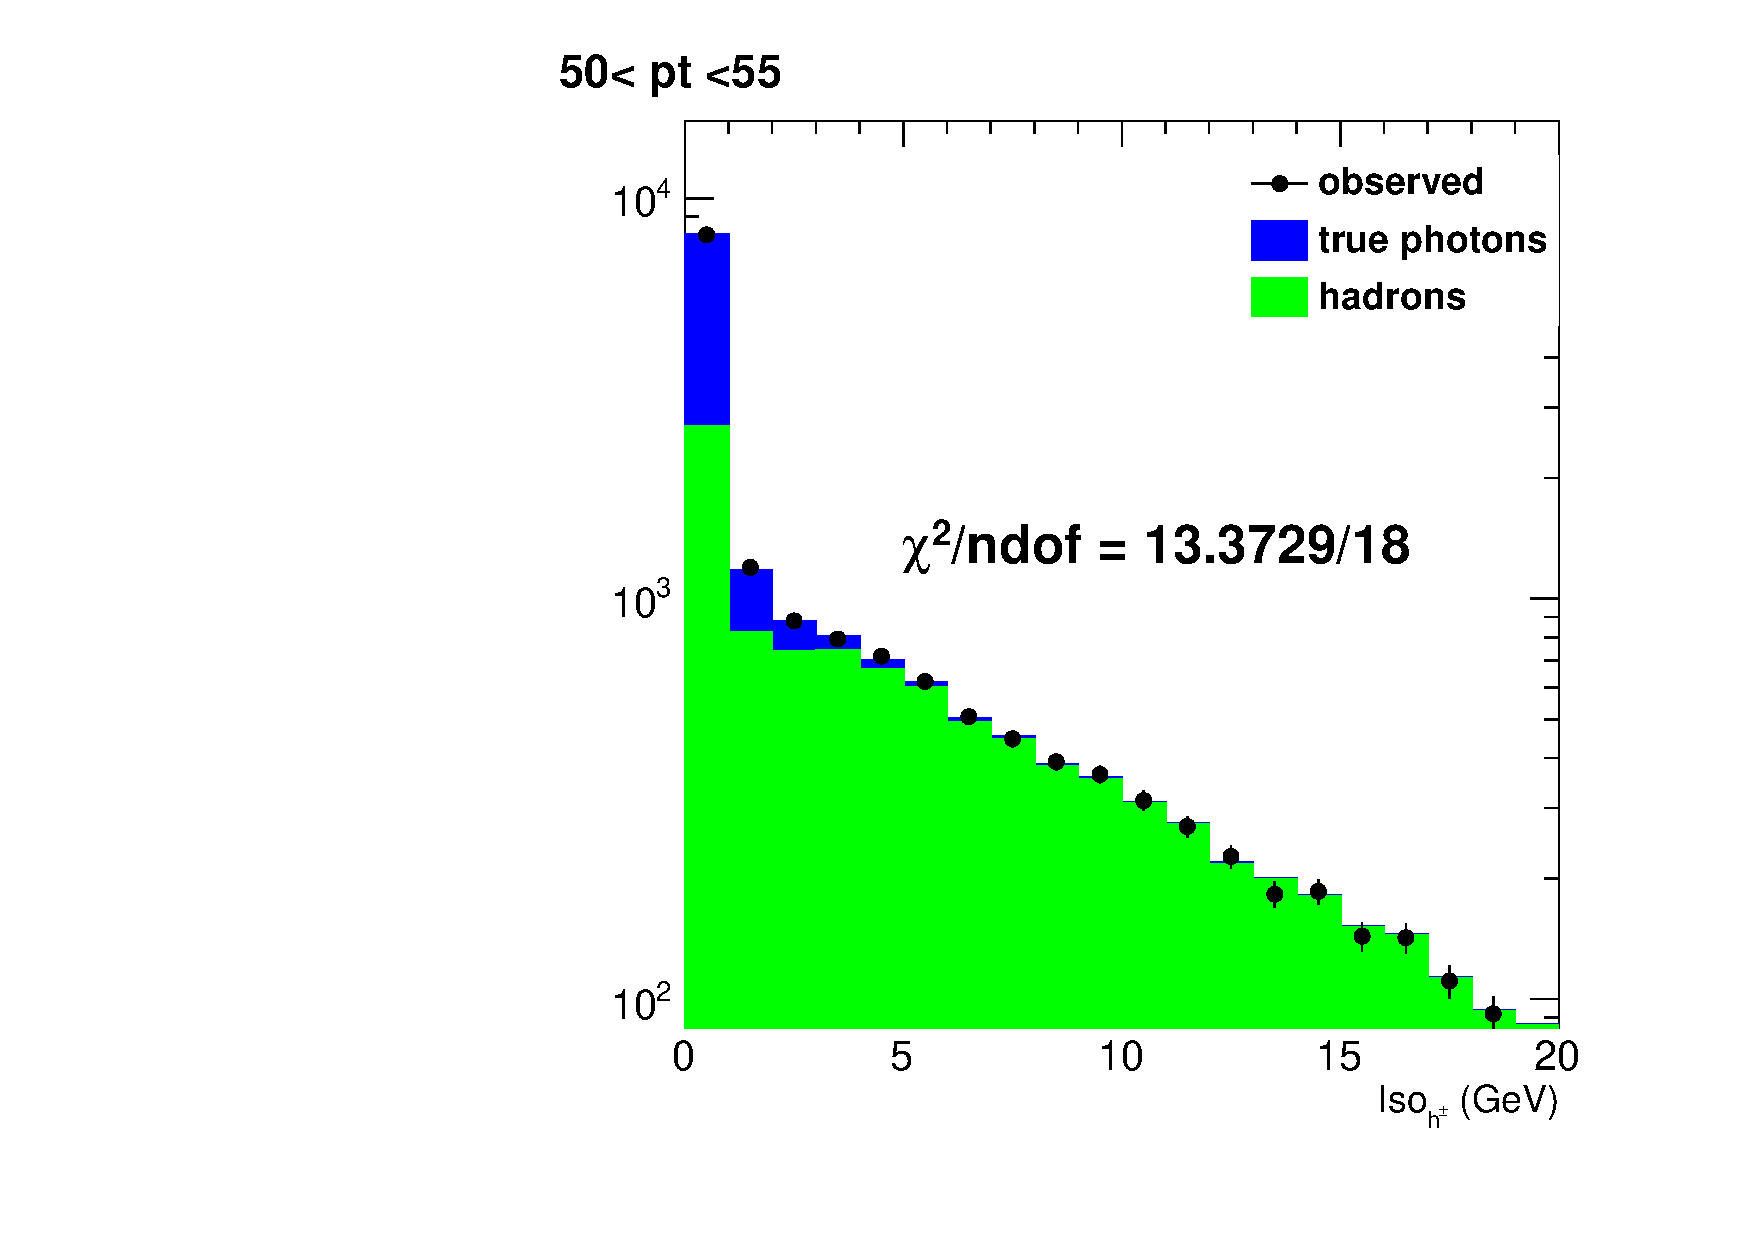
\includegraphics[width=0.32\textwidth]{Figures/frac-50-55_ChIso-DoubleEG-ReMiniAOD.pdf}         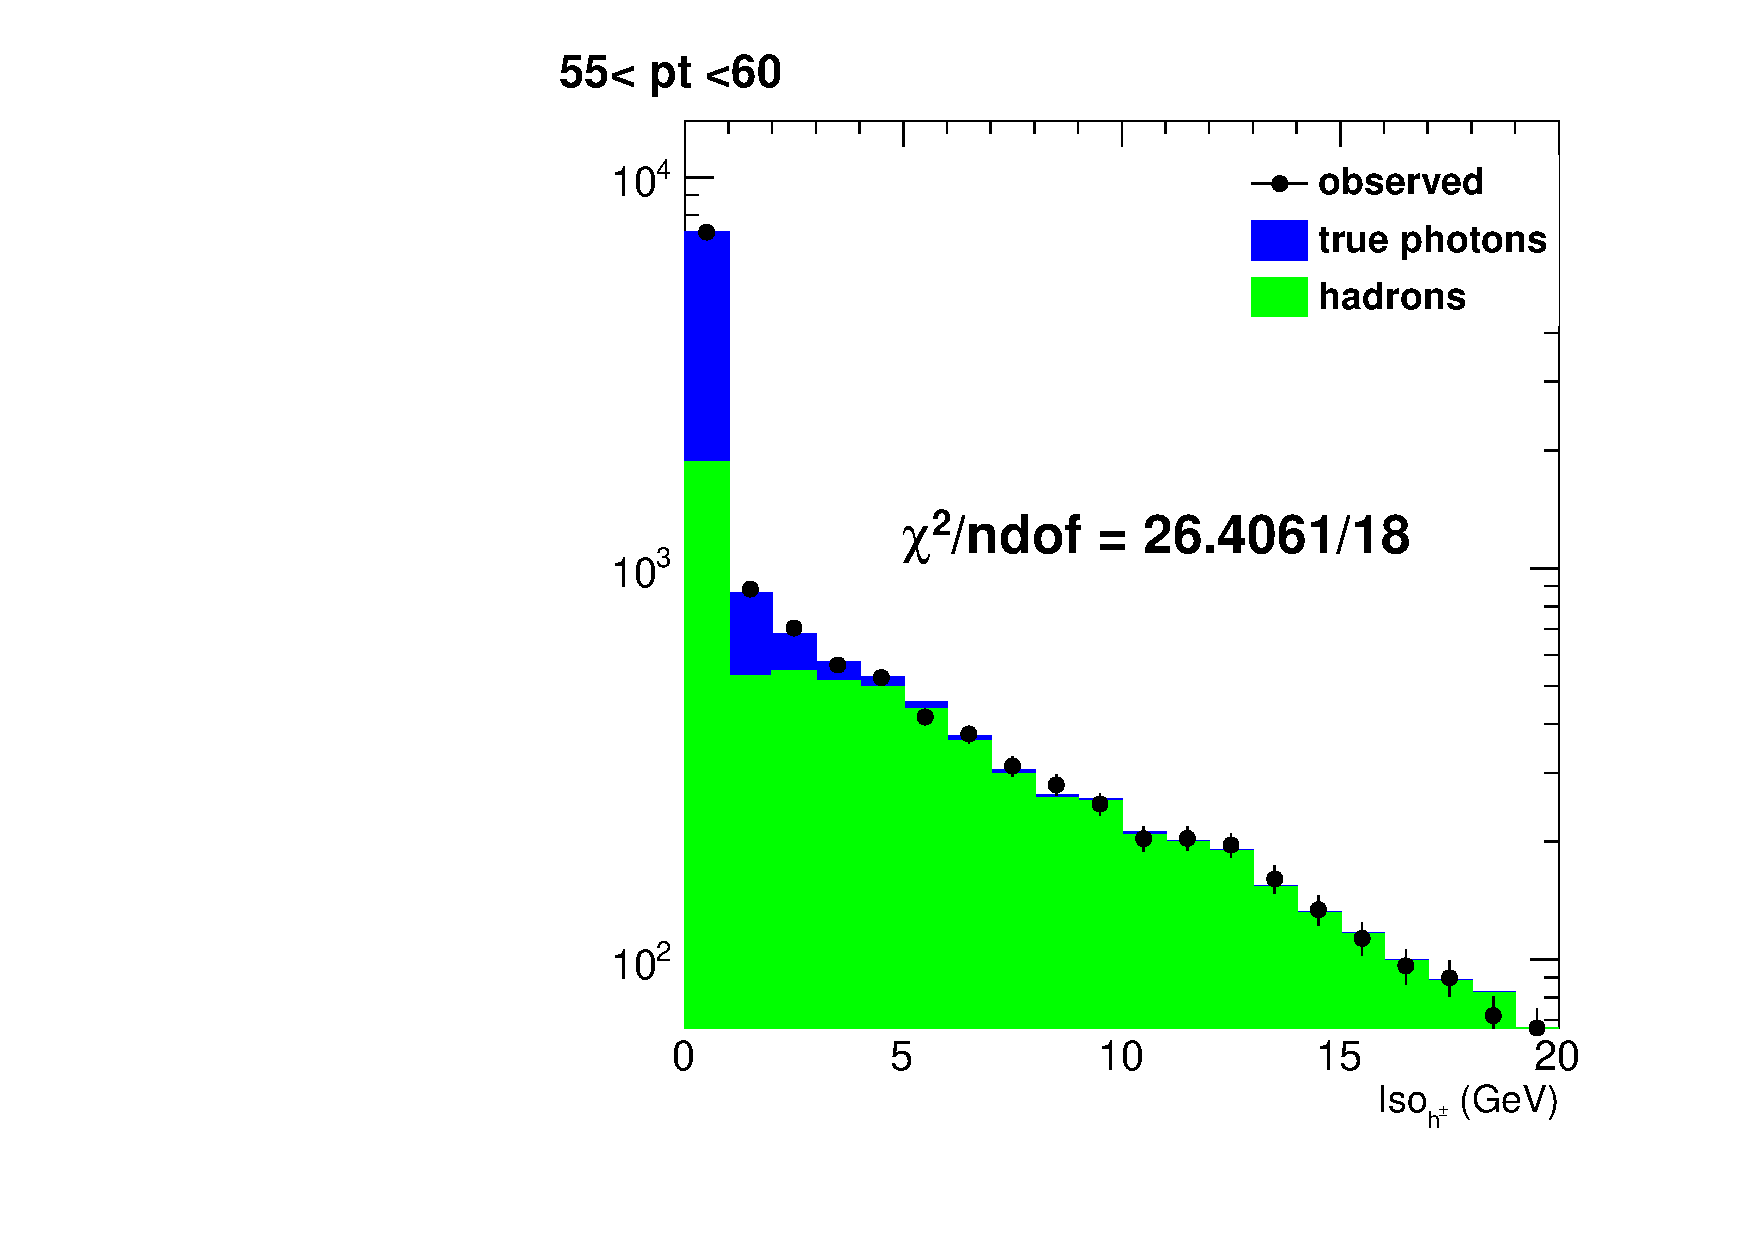
\includegraphics[width=0.32\textwidth]{Figures/frac-55-60_ChIso-DoubleEG-ReMiniAOD.pdf} \\
   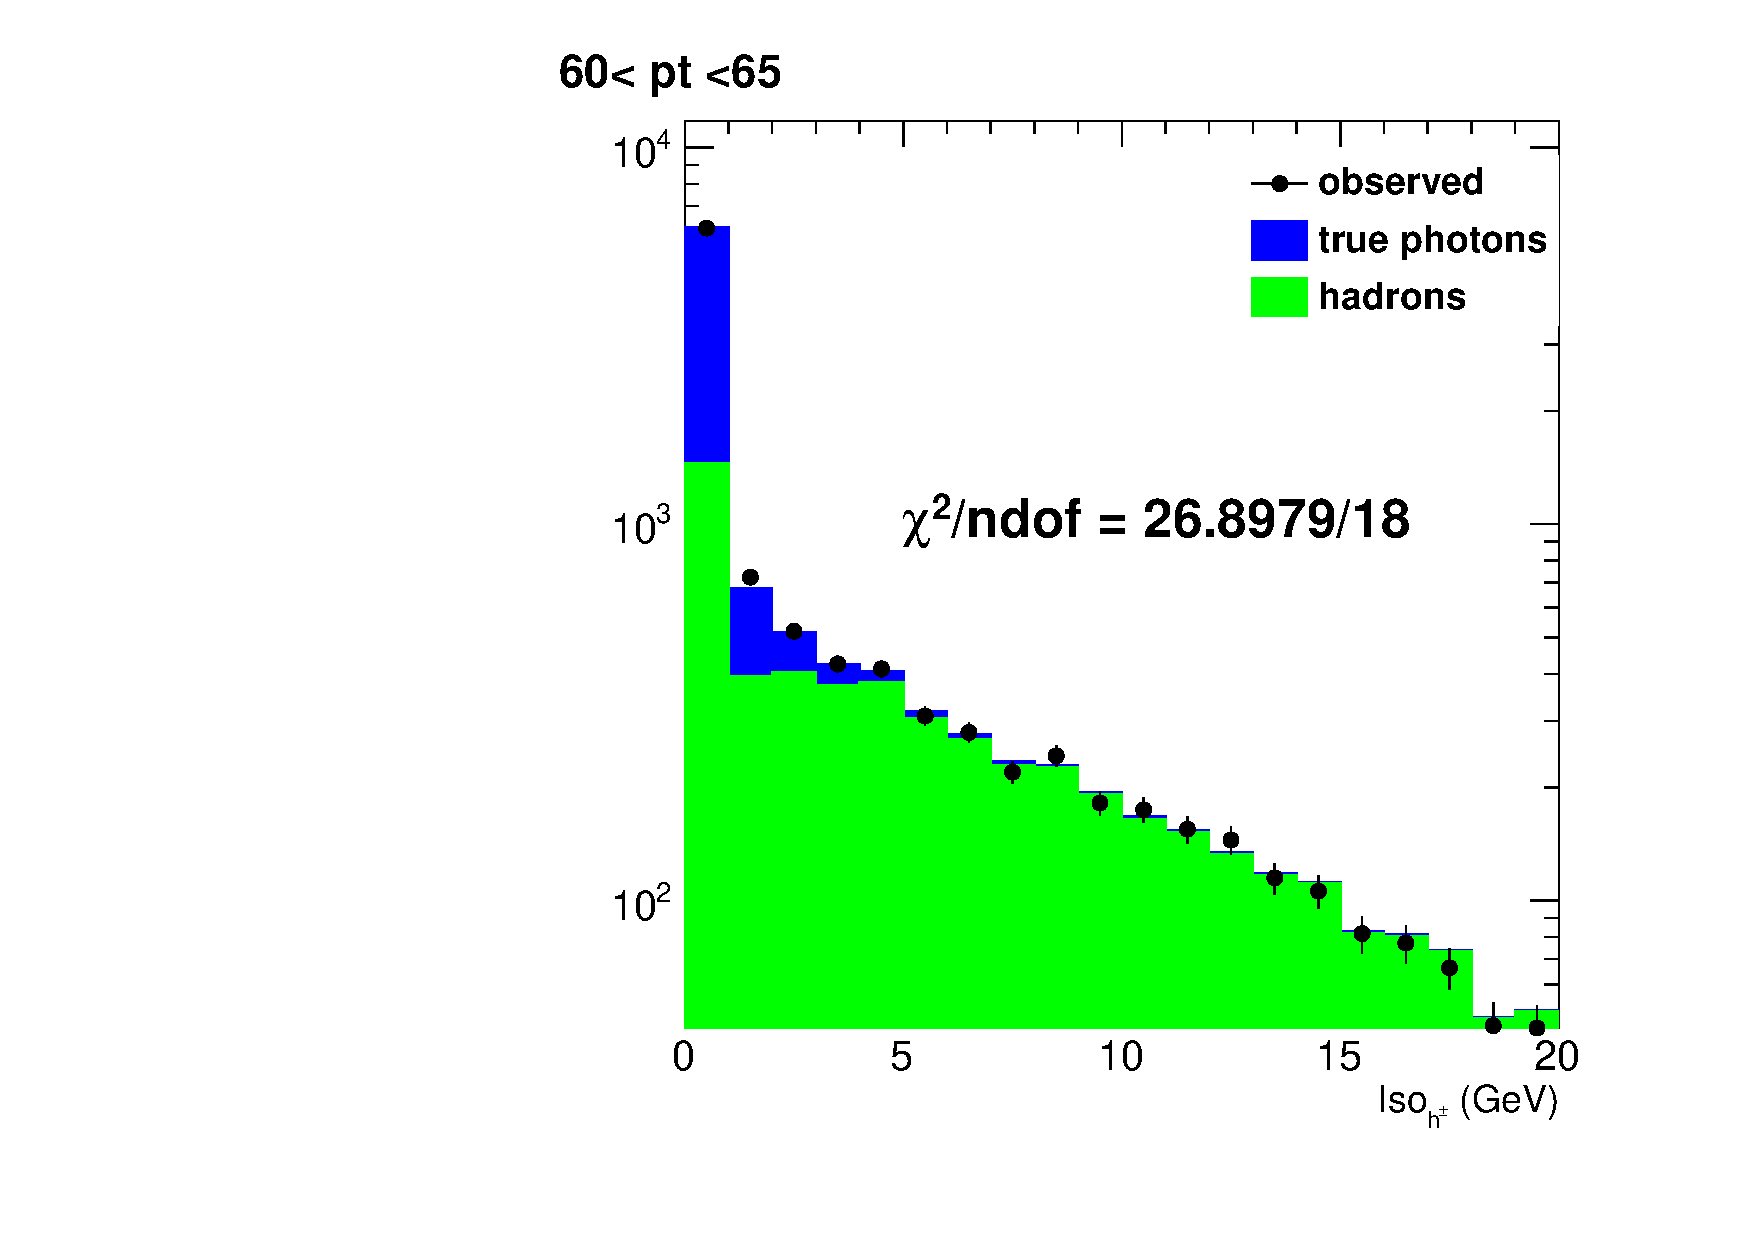
\includegraphics[width=0.32\textwidth]{Figures/frac-60-65_ChIso-DoubleEG-ReMiniAOD.pdf}   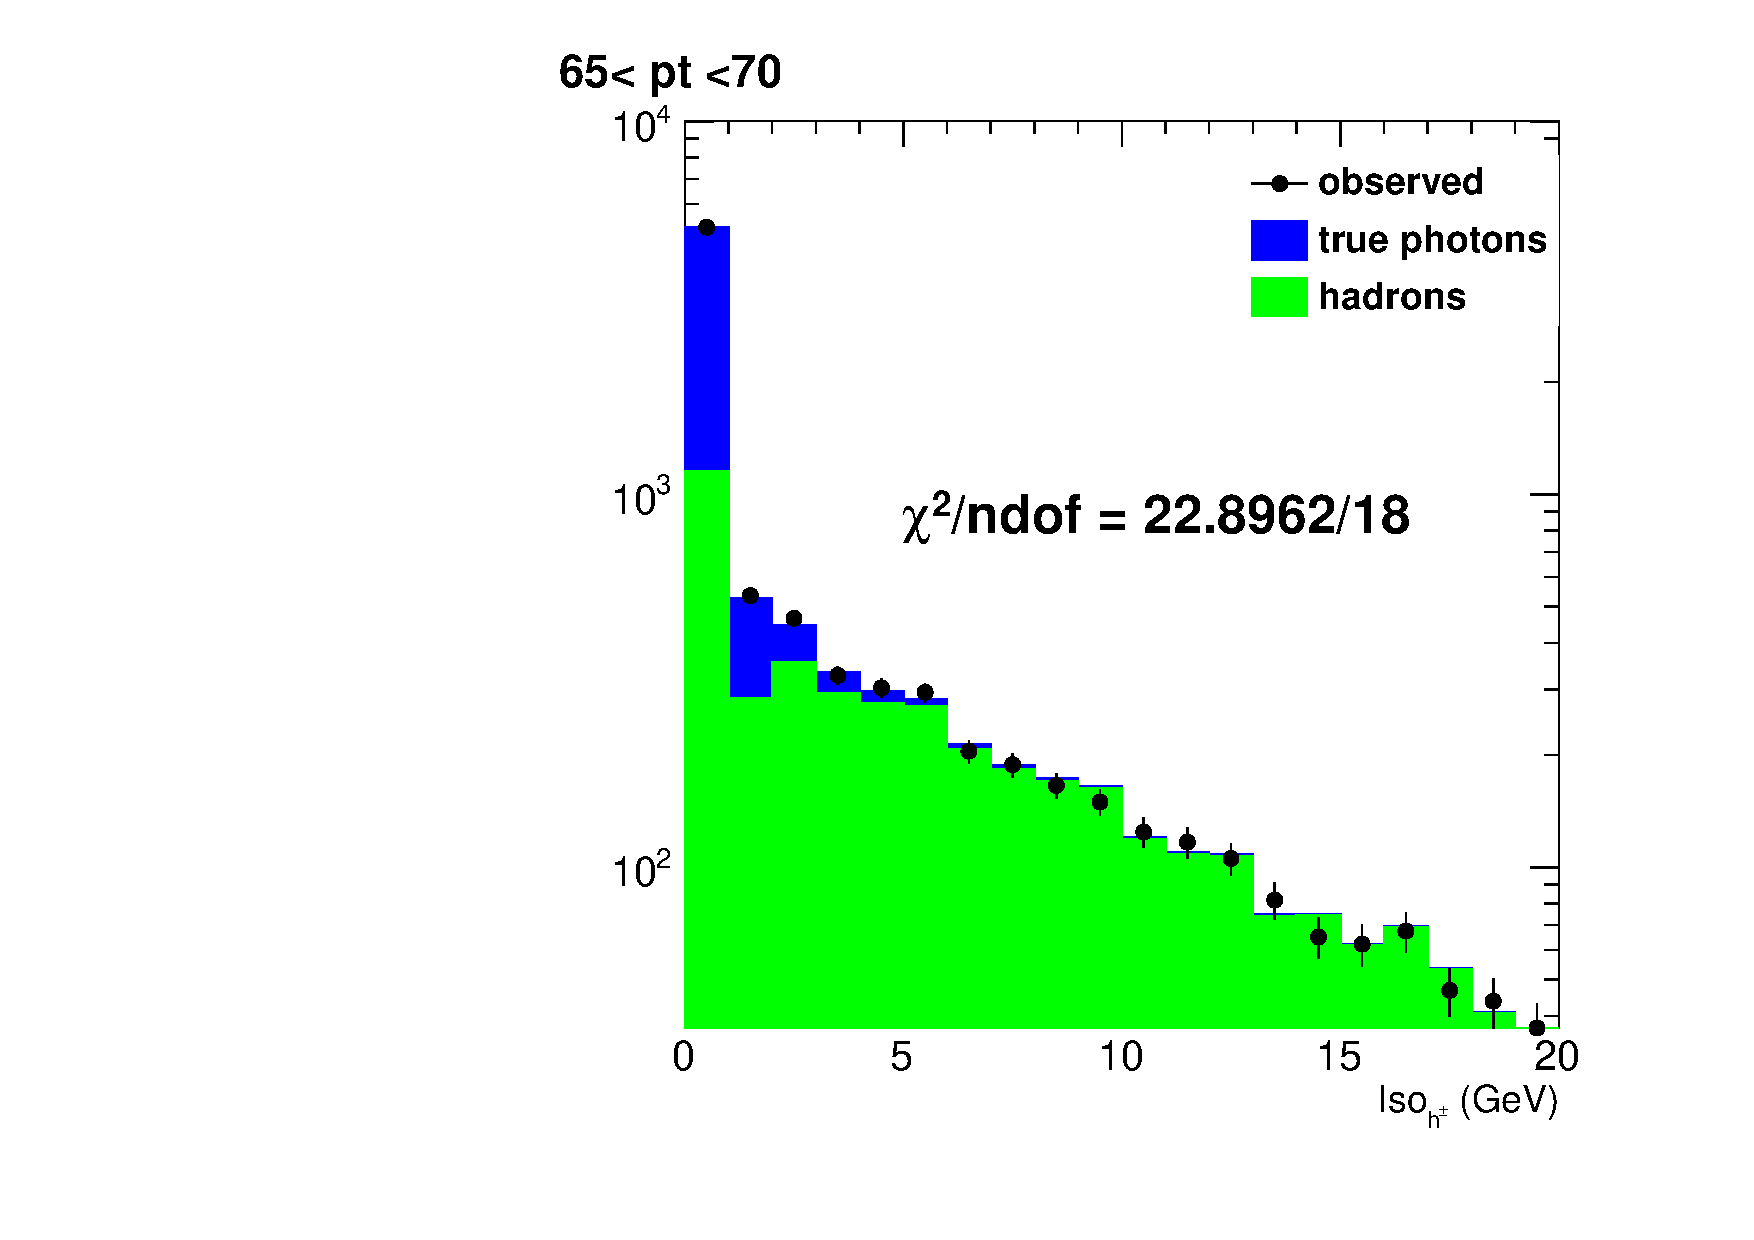
\includegraphics[width=0.32\textwidth]{Figures/frac-65-70_ChIso-DoubleEG-ReMiniAOD.pdf}         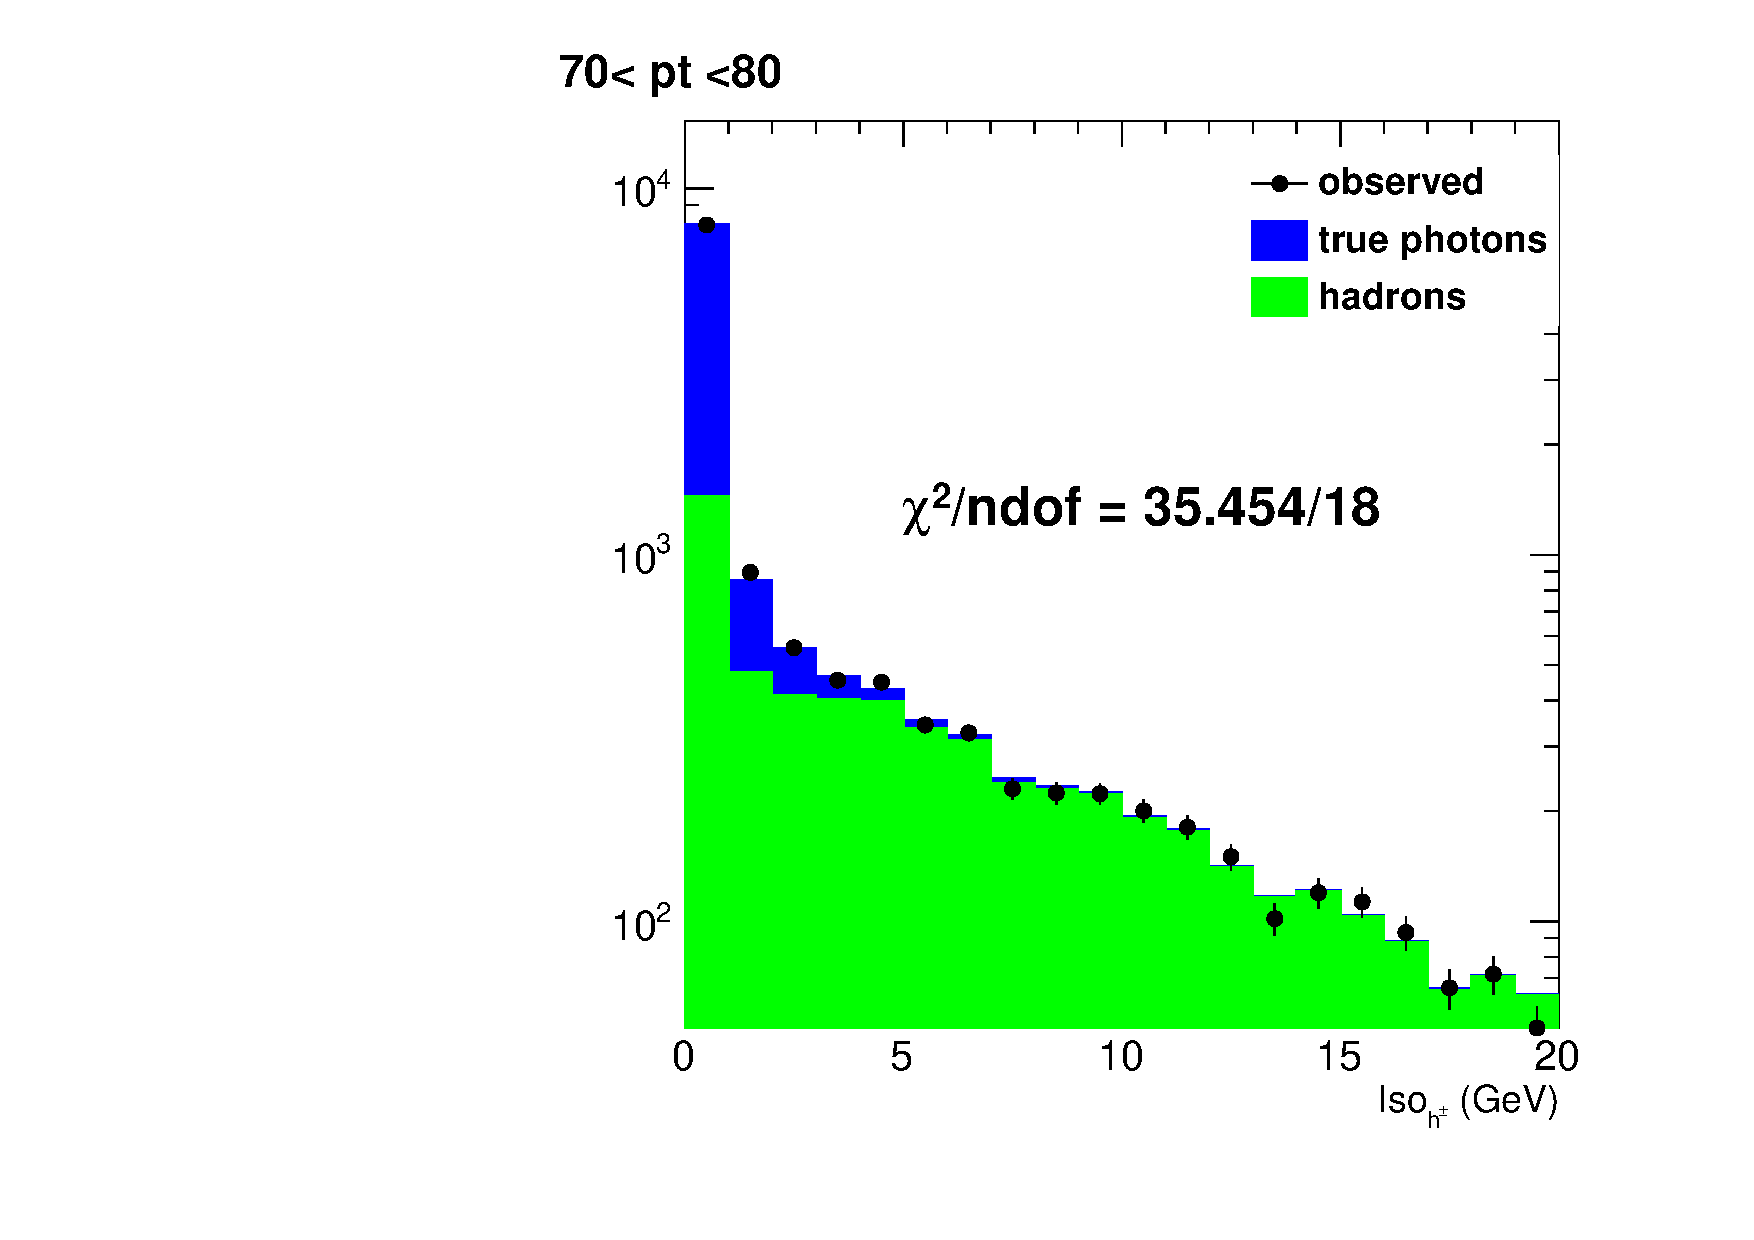
\includegraphics[width=0.32\textwidth]{Figures/frac-70-80_ChIso-DoubleEG-ReMiniAOD.pdf} \\
   \includegraphics[width=0.32\textwidth]{Figures/frac-80-90_ChIso-DoubleEG-ReMiniAOD.pdf}   \includegraphics[width=0.32\textwidth]{Figures/frac-90-120_ChIso-DoubleEG-ReMiniAOD.pdf}   \\
  \caption{Template fits for hadron fraction measurements in $e\gamma$ channel.}
 \label{fig:DoubleEGjetfakebins}
\end{figure}

\begin{figure}
  \centering
    \includegraphics[width=0.45\textwidth]{Figures/JetFakePho_DoubleEG_ReMiniAOD.pdf}
    \includegraphics[width=0.45\textwidth]{Figures/JetFakePho_MuonEG_ReMiniAOD.pdf}
  \caption{The hadron fractions estimated in DoubleEG (left) and MuonEG (right) dataset.} 
    \label{fig:hadronfraction}
\end{figure}

Once the fraction of fakes are determined, the number of fakes in the candidate photons can be calculated and used as the numerator sample for the transfer factor calculation. The denominator sample of the transfer factor is a jet-enriched proxy sample. This sample is formed by replacing the candidate photon with a proxy object, which fulfill the following  criteria:
\begin{center}
\begin{itemize}
\item pass H/E, $Iso_{pho}$, $Iso_{h^0}$ cut in the loose-ID
\item pass the pixel veto, electron veto and FSR veto
\item $\sigma_{i\eta i\eta} >$ 0.01031 \\
     or   1.29 $< Iso_{h^\pm} <$ 15 GeV
\end{itemize}
\end{center}

The transfer factor is then determined in the control region $p_{T}^{miss} <$ 70 GeV by calculating the ratio of numerator events to the denominators.\\

It is useful to parameterize the $p_T$ dependence of the transfer factors using analytical functions so that the result measured in low pt regions can be interpolated to the high $p_T$ region where statistics are limited. We choose to use a sum of two exponential functions to fit the photon $p_T$ spectrum. The fitting results are shown in Figure \ref{fig:jetFakePt}.

\begin{figure}
  \centering
    \includegraphics[width=0.45\textwidth]{Figures/JetFakeRate_transfer_eg_EB.pdf}
    \includegraphics[width=0.45\textwidth]{Figures/JetFakeRate_transfer_mg_EB.pdf}
  \caption{Function fits for jet-fake-photon transfer factor measurements in $e\gamma$ (left) and $\mu\gamma$ channel. The $p_T$ distributions of the proxy objects and fake photons are shown in black and red dots respectively. The one sigma band of the fitting are shown in black lines.}
    \label{fig:jetFakePt}
\end{figure}

From the fits, we obtained the function forms for the $e\gamma$ channel:
\begin{equation}
R_{fake/proxy} = \frac{ 1.43 \times 10^4 \cdot e^{-0.069 \cdot p_T} + 5.11 \times 10^2 \cdot e^{-0.030 \cdot p_T}}{4.08 \times 10^4 \cdot e^{-0.055 \cdot p_T} +  5.51 \times 10^2 \cdot e^{-0.019 \cdot p_T}}
\end{equation}

and $\mu\gamma$ channel:
\begin{equation}
R_{fake/proxy} = \frac{ 2.39 \times 10^4 \cdot e^{-0.082 \cdot p_T} + 3.33 \times 10^2 \cdot e^{-0.030 \cdot p_T}}{6.01 \times 10^4 \cdot e^{-0.059 \cdot p_T} +  5.90 \times 10^2 \cdot e^{-0.021 \cdot p_T}}
\end{equation}

The choice of the $\sigma_{i\eta i\eta}$ sideband is identified as the major source of systematic uncertainties of the fraction of fakes. Since the $Iso_{h^\pm}$ and $\sigma_{i\eta i\eta}$ are correlated, inaccuracy on the fake fraction estimation is expected even though the iterative method is applied. This uncertainty can be assessed by varying the sideband definition and repeating the fit with the modified template. We scan the lower bound of the sideband from 0.01031 to 0.0112 in a step of 0.0101, and scan the upper bound from 0.0140 to 0.0185 in a step of 0.0105. The scan result in one of the $p_T$ bin is shown in Figure \ref{fig:jetfakeSys}. The full variation is taken as the systematic uncertainty. 

\begin{figure}
  \centering
    \includegraphics[width=0.45\textwidth]{Figures/can2D-50-55_ChIso-DoubleEG-ReMiniAOD.pdf}
  \caption{2D distribution of the fraction of hadrons for photons with 50 GeV $< p_T <$ 55 GeV. The full variation will be used as systematic uncertainties of the template fit.}
    \label{fig:jetfakeSys}
\end{figure}


The systematic uncertainties on the fraction of fakes get propagated to the functional form of the fake photons via the $p_T$ spectrum fitting. To form the 1 $\sigma$ error band of the pt distribution, we performed toy MC experiments with the parameters and errors from the $p_T$ fitting. Assuming the fitting parameters have gaussian distributions around their nominal values, we construct a multi-variant Gaussian PDF using the nominal fitting values and their covariant matrix. 1000 sets of parameters are then generated from this Gaussian distribution. The 1 $\sigma$ band is formed by wrapping these toy distributions, as shown  in \ref{fig:jetFakePt}. 



\section{The Misidentification of Hadrons as Leptons}
\label{subsec:jetfakelep}

Events with jets and prompt photons also enter the signal region if the jets get misidentified as leptons. In this analysis,  we consider all leptons that do not originate  from a~\Wpm or~\PZz as  fakes. This includes leptons from heavy-flavour decays, misidentified jets, light-meson decays, and electrons from photon conversions. Studies on simulated QCD events show that the fake muons mostly come from  heavy flavor quarks, while the fake electrons predominantly come from light flavor jets with a significant electromagnetic components. 

We estimate the contribution of fake leptons in a manner analogous to the
estimation of fake photons: select a proxy sample of events enriched in the fake leptons, and then use a scale factor to extrapolate this sample to the background in the signal region.  The selection of the proxy sample is close to that of the signal candidate. We require the proxy sample to contain one candidate photon, one fake lepton proxy, and no candidate leptons. 

The scale factor for the fake lepton proxy sample is derived in a $40 < p_{T}^{miss} < 70\GeV$ control region using a template fit to the
$\Delta\phi\left(l, p_{T}^{miss}}\right)$ distribution. After removing the contribution of fake photons, events in the control region are dominated by $W\gamma/Z\gamma$ processes and fake lepton contributions. $p_{T}^{miss}$ in the fake lepton events usually come from mismeasured objects. Thus the $\Delta\phi\left(l, p_{T}^{miss}}\right)$ shape of the fake lepton background is different with that of the $W\gamma/Z\gamma$ processes. This feature allows us to perform a two templates fit to the $\Delta\phi\left(l, p_{T}^{miss}}\right)$ of the data and simultaneously determine the normalization for the fake lepton proxy sample and $W\gamma/Z\gamma$ simulated samples. The normalized proxy sample then provides the estimate of the
background contribution from events with fake leptons in the signal region. The template fit is described in details in Section~\ref{subsec:VG}. 

\subsubsection{Fake Electron Proxies}
We find from simulations of QCD events that fake electrons commonly result from light flavor jets which shower significantly in the ECAL and get misidentified as electrons. These fake electrons have some characteristic features like large energy sum around the objects,  broader cluster shapes in $\eta$, and less consistent match between the reconstructed track momentum and the corresponding cluster energy. We therefore impose the following requirements on the electron objects of our proxy sample:

\begin{itemize}
    \item Electron $\pt > 25\GeV$, $|\eta| < 1.442$ or $1.56 < |\eta| < 2.5$.
    \item Pass the medium H/E, $|\frac{1}{E}-\frac{1}{p}|$, nMissHits and conversion veto cuts
    \item Fail any of the $\sigma_{i\eta i\eta}$, $|\Delta\eta|$, $|\Delta\phi|$ and mini-isolation cuts. 
		\item mini-isolation $< 0.4$
\end{itemize}
From simulation, we find the selection has negligible contamination from prompt
electrons.

To check the consistency of the background modeling, we compare events in data
with proxy electrons to events in QCD simulation with electrons matched to
fakes. To ensure sufficient statistics in the QCD simulation, we replace the
requirement that the event contains a loose photon with the requirement that it
contains a loose jet, as described in Section \ref{subsec:jetID}, and we insist that
$\Delta R\left(\textrm{\Pl, jet}\right) > 0.8$. The distributions of several
kinematic variables are compared between the two samples, as shown in
Fig.~\ref{fig:c_electron}. Reasonable agreements are obtained in all distributions.
The $\Delta\phi\left(l, p_{T}^{miss}}\right)$ distribution
is used in the template fit to determine the normalization factor of the proxy
sample.

\begin{figure*}[hbtp]\begin{center}
    \includegraphics[width=0.475\textwidth]{Figures/faketemp_electron_met.pdf}
    \includegraphics[width=0.475\textwidth]{Figures/faketemp_electron_ht.pdf}
    \includegraphics[width=0.475\textwidth]{Figures/faketemp_electron_mt.pdf}
    \includegraphics[width=0.475\textwidth]{Figures/faketemp_electron_dPhi.pdf}
    \caption{Comparison of various kinematic distributions between simulated
        QCD events with a fake electron and events in data with a proxy
        electron. The distributions are area-normalized to facilitate a
        comparison of their shapes.}
        \label{fig:c_electron}
\end{center}\end{figure*}

\subsubsection{Fake Muon Proxies}

Simulation indicates that, in contrast to the electron case, muon fakes tend to
be the product of real, non-prompt muons from the decay of heavy-flavor quarks.
Because these are real muons, the distributions of their primary ID variables
tend to be indistinguishable from those of prompt muons. The primary handle for
distinguishing these objects is thus the mini-isolation variable, which tends
to be greater for objects produced in the decays of heavy quarks. We therefore
construct muon proxies by requiring candidate muons to pass the following
selection criteria:
\begin{itemize}
    \item Muon $p_T > 25\GeV$, $|\eta| <$ 2.4.
    \item Passes cut-based medium ID.
    \item $0.2 <$ mini-isolation $< 0.4$.
\end{itemize}
From simulation we conclude that the muon proxy sample has less than 5\%
contamination from prompt muons.

We again check the consistency of the background modeling by comparing the
kinematic distributions of data events with proxy muons to simulated events
with fake muons. We switch the requirement of a loose photon in the event
to the requirement of a loose jet, which is well separated from the lepton candidate
($\Delta R\left(\textrm{\Pl, jet}\right) > 0.8$). The distributions of these
variables are shown in Fig. \ref{fig:c_muon}. 

\begin{figure*}[hbtp]\begin{center}
    \includegraphics[width=0.475\textwidth]{Figures/faketemp_muon_met.pdf}
    \includegraphics[width=0.475\textwidth]{Figures/faketemp_muon_ht.pdf}
    \includegraphics[width=0.475\textwidth]{Figures/faketemp_muon_mt.pdf}
    \includegraphics[width=0.475\textwidth]{Figures/faketemp_muon_dPhi.pdf}
    \caption{Comparison of various kinematic distributions between simulated
        QCD events with a fake muon and events in data with a proxy muon. The
        distributions are area-normalized to facilitate a comparison of their
        shapes.}
        \label{fig:c_muon}
\end{center}\end{figure*}

\subsubsection{Corrections on Proxy Samples}
Because the mini-isolation is computed using a cone size depending on the momentum of the lepton, the mini-isolation cuts could have non-linear efficiencies. Thus the $p_T$ distribution of the fake lepton background may not be perfectly modeled by the proxy sample. By comparing the $p_T$ distribution of the fake proxies and simulated QCD events, we find disagreements in the fake electron $p_T$ shapes. Though the lepton $p_T$ is not directly used in defining the signal bins, a mismodeled lepton $p_T$ could still affect the determination of the $V\gamma$ and fake lepton scale factors. Therefore, we use the ratios between the simulated events and fake electron proxies as correction factors to reweight the fake electron control samples. For the fake muons, the shape of the proxy sample is more consistent with the QCD simulations, moreover, the rate for a jet to be misidentified as a muon is much smaller than that of an electron. Thus we won't correct the muon control samples. 
Figure \ref{fig:reweight_fakelep} shows the $p_T$ distributions and the MC-to-data ratios. Table \ref{table:correctionsfakelep} summarize the correction factors we used for the electron proxy reweighting.

\begin{figure*}[hbtp]\begin{center}
    \includegraphics[width=0.475\textwidth]{Figures/faketemp_electron_LepPt.pdf}
    \includegraphics[width=0.475\textwidth]{Figures/faketemp_muon_LepPt.pdf}
    \caption{Comparison of lepton $p_T$ distributions between the QCD simulation and fake lepton proxy samples. Left: $e\gamma$ events, right: $\mu\gamma$ events. The ratio can be used as correction factors.}
        \label{fig:reweight_fakelep}
\end{center}\end{figure*}

\begin{table}[htdp]
	\centering
  \begin{tabular}{|c|c|c|}
  \hline
  $p_T$ (GeV)  & $e$ proxy corrections \\ \hline
  25-50  & 0.79$\pm$ 0.02  \\ \hline
  50-75  & 1.12$\pm$ 0.04  \\ \hline
  75-100 & 1.41$\pm$ 0.08  \\ \hline 
  100-125& 1.67$\pm$ 0.14  \\ \hline 
  125-150& 2.05$\pm$ 0.23  \\ \hline 
  150-200& 1.73$\pm$ 0.23  \\ \hline
  200-400& 1.55$\pm$ 0.27  \\ \hline
  $>$ 400& 1.0 \\ \hline 
  \end{tabular}
  \caption{Correction factors used in electron proxy reweighting.}
  \label{table:correctionsfakelep}
\end{table}

\section{$W\gamma$ and $Z\gamma$ Background}\label{subsec:VG}
The standard model production of W or Z boson in associate with a photon is the major background of this search. Since the cross section measurment of this process at 13 TeV is not published yet, and the calculated cross section for WW and WZ processes show diviations from measured results, this background is estimated by scaling the simulated samples by a factor derived in the control region using a template fit. \\ 

The $W\gamma$ sample is formed by mixing the inclusive $WGToLNuG$ sample with two $p_T$-binned samples: WGJets\_MonoPhoton\_PtG-40to130 and WGJets\_MonoPhoton\_PtG-130. The former one is truncated at 50 GeV and the high-statistics $p_T$-binned samples are used for $p_T$ above 50 GeV. All of the three $W\gamma$ samples are generated with MadGraph at leading order. To account for higher order corrections, a constant NNLO k-factor of 1.34 is applied. Figure \ref{fig:mixWG} shows that a smooth photon $p_{T}$ distribution can be obtained via this mixing procedure. For the $Z\gamma$ process, we use an inclusive NLO sample with $p_T >$ 10 GeV. Because the $Z\gamma$ sample has a $M_{ll} > 30$ GeV cut at metrix-element level, we use part of the Drell-Yan samples to supplement the events with $M_{ll} < 30$ GeV. All of these simulated samples are then normalized to $35.87 fb^{-1}$ and mixed to form the $V\gamma$ template.

\begin{figure}
  \centering
    \includegraphics[width=0.45\textwidth]{Figures/WGMixing.pdf}
  \caption{Photon $p_T$ distributions in individual $W\gamma$ samples and their combination.}
    \label{fig:mixWG}
\end{figure}

The initial state radiation (ISR) can affect the kinematic quantities of the simulation. Studies using $Z\gamma\rightarrow\mu\mu\gamma$ events show that there is a systematic discrepancy between the data and simulated events. To improve the modeling of the $V\gamma$ samples, we assign each simulated event a correction factor according to its ISR $p_T$. The ISR $p_T$ is calculated using the ISR-jet counting algorithm \cite{ISR-JET-ALGO}. Derivation of the correction factors is described in Appendix A. 

Because the angular distance between the signal lepton and MET has different shapes in the $V\gamma$ and misidentified object background, we choose to use $\Delta\phi(l,E_{T}^{miss})$ as the distribution for the template fit. For the fake lepton background, the missing transverse momentum is typically caused by mismeasured object and tends to be aligned with the lepton. The $W\gamma$ events, on the other hand, has a neutrino and thus contains genuine $E_{T}^{miss}$. Figure \ref{fig:dphitemplate} shows the distribution of these two sources. Fitting the two $\Delta\phi$ templates to the distributions of the data will simultaneously determine the normalization factors for the $V\gamma$ and fake leptons backgrounds. 

\begin{figure}
  \centering
    \includegraphics[width=0.45\textwidth]{Figures/dphiTemplate_eg.pdf}
    \includegraphics[width=0.45\textwidth]{Figures/dphiTemplate_mg.pdf}
  \caption{$\Delta\phi(l,E_{T}^{miss})$ distribution of the $V\gamma$ sample (blue) and fake lepton template(red) in the $e\gamma$ channel (left) and $\mu\gamma$ channel (right). }
    \label{fig:dphitemplate}
\end{figure}

The template fitting is performed in the control region, defined by 40 GeV $< p_{T}^{miss} <$ 70GeV. The lower cut is applied to suppress $Z\gamma$ events. Figure \ref{fig:WGZG_met} shows the normalized $p_{T}^{miss}$ distribution of the $W\gamma$ and $Z\gamma$ samples. By applying a 40 GeV $p_{T}^{miss}$ cut, we select a control sample dominated by $W\gamma$ events.  

\begin{figure}
  \centering
    \includegraphics[width=0.45\textwidth]{Figures/dphiTemplate_MET.pdf}
  \caption{$p_T^{miss}$ distributions of the $W\gamma$ (red) and $Z\gamma$ (blue) sample. The 40 GeV cut will remove a large fraction of the $Z\gamma$ contributions.}
    \label{fig:WGZG_met}
\end{figure}

The target distribution of this template fit is the $\Delta\phi(l,p_{T}^{miss})$ shape of the data in the control region, with fake photon and rare EWK backgrounds subtracted. Two templates are then selected, one from the $V\gamma$ sample and the other one from the fake lepton samples. The fit is performed with the ROOFIT package using the binned maximum likelihood estimator.

Once the fraction of $V\gamma$ events in the control region is determined, the scale factor for the $V\gamma$ sample can be calculated as: 
\begin{equation}
 		a_{V\gamma} = \frac{N_{con}\times f_{V\gamma}}{N_{V\gamma}}, 
\end{equation}\\
where $N_{con}$ is the total number of events in the control sample, $f_{V\gamma}$ is the fraction of $V\gamma$ events derived from the template fit, and $N_{V\gamma}$ is the number of events in the $V\gamma$ template. After removing the $V\gamma$ events, the remaining events in the control sample are the contribution of fake leptons. 

%To study the possible $p_T$ dependence of the $V\gamma$ scale factors, we perform the template fit in four lepton $p_T$ bins: (25-50, 50-70, 70-100, $>=$100) GeV. Figure \ref{fig:dphiptdependence} shows that the fluctuation of the scale factors in different $p_T$ bins are within systematic uncertainties. Since no obvious $p_T$ dependence is observed and the statistics at high $p_T$ is limited, we decide to perform the template fit in the full $p_T$ range and use a global $V\gamma$ scale factor. However, this may not be true for the fake lepton scale factors, because the $p_T$ distribution of the fake lepton background may not be perfectly modeled by the proxy sample. Thus we first subtract the $V\gamma$ contribution from the control sample using the global $V\gamma$ scale factors, and then use $p_T$-binned fake lepton scale factors to let the fake lepton proxy sample fill the control region. The $p_T$-binned scale factors are obtained by taking the ratio of the remaining events to the fake lepton templates in different $p_T$ bins. Figure \ref{fig:dphifitresult} shows the result of the fit. 

To study the possible $p_T$ dependence of the $V\gamma$ scale factors, we perform the template fit in four lepton $p_T$ bins: (25-50, 50-70, 70-100, $>=$100) GeV. Figure \ref{fig:dphiptdependence} shows that the fluctuation of the scale factors in different $p_T$ bins are within systematic uncertainties. Since no obvious $p_T$ dependence is observed and the statistics at high $p_T$ is limited, we decide to perform the template fit in the full $p_T$ range and use a global $V\gamma$ scale factor. Figure \ref{fig:dphifitresult} shows the result of the fit. 
\begin{figure}
  \centering
    \includegraphics[width=0.45\textwidth]{Figures/scale_ptDependence_eg.pdf}
    \includegraphics[width=0.45\textwidth]{Figures/scale_ptDependence_mg.pdf}
  \caption{The $V\gamma$ scale factors as a function of lepton $p_T$. The blue dots denote the $p_T$ binned scale factors, and the black dots denote the scale in full $p_T$ range. Left: $e\gamma$ channel, right: $\mu\gamma$ channel. }
    \label{fig:dphiptdependence}
\end{figure}


\begin{figure}
  \centering
    \includegraphics[width=0.45\textwidth]{Figures/fit_dPhi_eg_0_1000_met40_iso4.pdf}
    \includegraphics[width=0.45\textwidth]{Figures/fit_dPhi_mg_0_1000_met40_iso4.pdf}
  \caption{Results of the $\Delta\phi(l,E_{T}^{miss})$ template fit in the $e\gamma$ channel (left) and $\mu\gamma$ channel (right).}
    \label{fig:dphifitresult}
\end{figure}

The resulting scale factors for the $e\gamma$ channel are:

\begin{eqnarray*}
	a_{V\gamma(e)} &=& 1.17 \pm 0.23 \\
	a_{fake(e)}  &=& 0.24 \pm 0.05
\end{eqnarray*}

and for the $\mu\gamma$ channel are:

\begin{eqnarray*}
	a_{V\gamma(\mu)} &=& 1.33 \pm 0.26 \\
	a_{fake(\mu)}  &=& 0.62 \pm 0.12
\end{eqnarray*}


The majors systematic uncertainties of this estimation come from the shapes of the fitting target and data-to-simulation ESF applied to the Vgamma samples. To evaluate the size of the uncertainty, we use toy MC to vary the Vgamma distribution and the contribution from the fake photon background, and 
repeat the fit 1000 times. Figure \ref{fig:dphisystematic} shows the distribution of the scale factors of these 1000 toy tests. This method reveald a 20\% systematic uncertainty on the scale factor.

\begin{figure}
  \centering
    \includegraphics[width=0.45\textwidth]{Figures/VGammaScale_eg.pdf}
    \includegraphics[width=0.45\textwidth]{Figures/VGammaScale_mg.pdf}
  \caption{Distribution of the scale factors derived from 1000 toy MC experiments. Left: $e\gamma$ channel, right: $\mu\gamma$ channel.}
    \label{fig:dphisystematic}
\end{figure}

\section{Systematic Uncertainties}
The relative systematic uncertainties on the background estimation and signal expectation are listed in Table \ref{table:ch4-systematic}. For the fake photon backgrounds, systematic uncertainties are obtained using toy MC methods, as described in Section \ref{subsec:efakepho}\ref{subsec:jetfakepho}. The same method is also used in determining the uncertainties of the scale factors for the fake lepton and $V\gamma$ backgrounds, as described in Section \ref{subsec:VG}. Possible errors on the $V\gamma$ scales, including uncertainties on cross sections, luminosity, trigger and object identification efficiencies, have been absorbed into the scale factors. In addition to the overall scale, uncertainties caused by the ISR reweighting are also considered. We use the corrected distributions as the central values, and take the full corrections as the systematic uncertainties.

For the backgrounds that are taken from simulation, systematic uncertainties can arise from cross sections, luminosity, and jet energy measurements.  Follow the recommendation of the luminosity study group, we assign a 2.6\% uncertainty on the integrated luminosity. For the rare background, a 50\% uncertainty on the cross section is assumed, covering the difference between calculated cross sections and latest CMS measurements. Uncertainties on jet energy scale (JES) and jet energy resolution (JER) are evaluated by varying the jet energy corrections by $\pm\sigma$ and counting the changes in each signal bin.

The number of events of the fake object proxy samples are limited, especially in the high $p_T^{\gamma}$ and high $p_T^{miss}$ bins which contains very little fake object backgrounds. Therefore we use gamma distribution and estimated transfer factors to model the statistical uncertainties of these backgrounds. This allow us to assign uncertainties on the bins which have zero event in the proxy sample. 

\begin{table}[htdp]
	\centering
  \resizebox{\linewidth}{!}{
  \begin{tabular}{|c||c||c|c|c|c|c|}
  \hline
  source of uncertainties   & SUSY Signal &  $e\rightarrow\gamma$ fakes & jet$\rightarrow\gamma$ fakes & jet$\rightarrow l$ fakes & $V+\gamma$  & rare EWK \\ \hline
	Jet energy scale          & 0-10\%      &  -                          &  -                           & -                        &  0-15.6\%   & 0-24.8\% \\ \hline       
	Jet energy resolution     & 0-10\%      &  -                          &  -                           & -                        &  0-13.6\%   & 0-23\%   \\ \hline
	ID, trigger ESF           & 4\%         &  -                          &  -                           & -                        &  1.4-6.5\%  & 1.3-6.5\% \\ \hline
	e-fake-photon shape       & -           &  8.0-50.5\%                 &  -                           & -                        &             &           \\ \hline
	jet-fake-photon shape     & -           &  -                          &  7.9-55.8\%                  & 0-42.4\%                 &  -          & -         \\ \hline
	ISR corrections           & -           &  -                          &  -                           & -                        &  2.6-57.8\% & -         \\ \hline
	Cross section             &	4.3-36.8\%  &  -                          &  -                           & -                        &  -          & 50\%      \\ \hline
	normalization scale       & -           &  -                          &  -                           & 20\%                     &  20\%       & -         \\ \hline
	Integrated luminosity     & 2.6\%       &  -                          &  -                           & -                        &  -          & 2.6\%     \\ \hline	
  \end{tabular}
	}
  \caption{Systematic uncertainties of the SUSY signals and SM backgrounds.}
  \label{table:ch4-systematic}
\end{table}


\section{Validation of the Background Prediction}

The $M_T(l, p_{T}^{miss}) < 100$ GeV region is dominated by background events. Studies with TChiWG and T5WG samples show that this region has negligible signal contamination. Therefore, we propose to use $M_T < 100$ GeV as a validation region to test the background prediction, especially the modeling of $p_T^{miss}$ distribution. Figure \ref{fig:etvalidation},\ref{fig:metvalidation}, and \ref{fig:htvalidation} show the comparison between the data and background prediction in the validation region. A good agreement is obtained in both channels.

\begin{figure}
  \centering
    \includegraphics[width=0.7\textwidth]{Figures/VALID_egamma_2016ReMiniAOD_pt.pdf} \\
    \includegraphics[width=0.7\textwidth]{Figures/VALID_mg_2016ReMiniAOD_pt.pdf} \\
  \caption{Photon $p_T$ distributions in the $e\gamma$ channel (top) and the $\mu\gamma$ channel (bottom).}
    \label{fig:etvalidation}
\end{figure}

\begin{figure}
  \centering
    \includegraphics[width=0.7\textwidth]{Figures/VALID_egamma_2016ReMiniAOD_met.pdf} \\
    \includegraphics[width=0.7\textwidth]{Figures/VALID_mg_2016ReMiniAOD_met.pdf} \\
  \caption{$p_T^{miss}$ distributions in the $e\gamma$ channel (top) and the $\mu\gamma$ channel (bottom).}
    \label{fig:metvalidation}
\end{figure}

\begin{figure}
  \centering
    \includegraphics[width=0.7\textwidth]{Figures/VALID_egamma_2016ReMiniAOD_HT.pdf} \\
    \includegraphics[width=0.7\textwidth]{Figures/VALID_mg_2016ReMiniAOD_HT.pdf} \\
  \caption{HT distributions in the $e\gamma$ channel (top) and the $\mu\gamma$ channel (bottom).}
    \label{fig:htvalidation}
\end{figure}

\end{document}
